%% =====================================================================
%% Manuscript for GIScience & Remote Sensing (Taylor & Francis, tgrs20)
%% Taylor & Francis "Interact" LaTeX template, APA (author-date) references
%% ---------------------------------------------------------------------
%% Needs: interact.cls (download the "Interact" LaTeX template from
%%        Taylor & Francis Author Services and put interact.cls next to
%%        this file) and apacite (in TeX Live / MiKTeX).
%% Compile: pdflatex -> bibtex -> pdflatex -> pdflatex
%% Search for "TODO" to find every place that still needs your input.
%% =====================================================================

%% xcolor is loaded by the class or later packages; pass the table option
%% up front so it never causes an option clash.
\PassOptionsToPackage{table}{xcolor}

\documentclass[]{interact}

\usepackage[utf8]{inputenc}
\usepackage[T1]{fontenc}
\usepackage{epstopdf}        % allows EPS figures with pdflatex

%---- Maths -----------------------------------------------------------
\usepackage{amsmath}
\usepackage{amssymb}
\usepackage{mathtools}
\usepackage{bm}

%---- Tables / floats (all used by the appendix tables) --------------
\usepackage{booktabs}
\usepackage{array}
\usepackage{multirow}
\usepackage{makecell}
\usepackage{longtable}
\usepackage{threeparttable}
\usepackage{xcolor}
\usepackage{rotating}
\usepackage{float}           % [H] placement in the appendix
\usepackage[caption=false]{subfig}
\usepackage{enumitem}

%---- Line numbers (helpful for reviewers) ----------------------------
\usepackage{lineno}

%---- References: T&F APA style via apacite (keeps \citep / \citet) --
\usepackage[natbibapa,nodoi]{apacite}
\setlength\bibhang{12pt}
\renewcommand\bibliographytypesize{\fontsize{10}{12}\selectfont}

%---- Links (load last; only if the class has not already) ------------
\makeatletter
\@ifpackageloaded{hyperref}{}{\usepackage{hyperref}}
\makeatother
\AtBeginDocument{\hypersetup{hidelinks}}

\articletype{Research Article}

\begin{document}

%% ---- Title ---------------------------------------------------------
\title{Quantification of Ghana's historical mining expansion: Back-casting from a recent mine inventory}

%% ---- Author --------------------------------------------------------
%% Peer review is single-anonymous, so author details stay in the file.
%% ORCID (0009-0002-1884-5944) is entered in the submission system.
\author{
\name{Hannes Br\"auer\textsuperscript{a}\thanks{CONTACT Hannes Br\"auer. Email: hannes.brauer@nmbu.no}}
\affil{\textsuperscript{a}Department of International Environment and Development Studies,
Norwegian University of Life Sciences (NMBU), \AA s 1432, Norway}
}

\maketitle

%% ---- Abstract: unstructured, max. 500 words (GRS) ------------------
\begin{abstract}
Ghana has witnessed a rapid expansion of mining, especially in its
south-western forest zone. This expansion is visible and measurable from
space using remote sensing, and introduces profound changes for people
living in these areas. Accurately quantifying the timing and extent of
mining is important to evaluate policies, sustainability, and
development outcomes but is complicated by cloud cover and poor-quality imagery
in earlier Landsat years (pre-2013). In this study, I am developing annual mining
footprints for all of Ghana based on high-resolution mapping of mines in 2019.
Using Landsat imagery from 2000 through 2019 (27 spectral, index, texture and
terrain bands), training a national random forest (RF) classifier to detect mining,
vegetation, and water, and applying backward transition rules to prevent implausible
class reversions, I estimate historical mining expansion within known mining boundaries.
Under spatially blocked cross-validation with a variogram-derived buffer, the model reaches
an overall accuracy of 0.87 and a mining $F_1$ of 0.78, with zone-specific models not performing better.
I validate my approach by drawing 1000 Monte Carlo simulations from a bootstrapped ensemble,
and comparing industrial mining onset to industry statistics and an independent convolutional
neural network (CNN). I find that constraining classification to known mining areas enables
an improved assessment of mining-related land conversion which includes mine infrastructure
and tailings, while backward transition rules prevented implausible pixel transitions between landcover
classes due to low data quality. Results indicate Ghana's mining area expanded
from approximately 1\,623~ha in 2000 to 53\,391~ha in 2019, with peak expansion
occurring during 2012 and 2013, and from 2016 onwards. My approach demonstrates that recent improvements
in remote sensing can be used to train classification models for better historical analyses of
lower resolution and lower quality imagery. The results show how recent high-resolution imagery
can contribute to improving inferences from existing low-resolution imagery, enabling time-series analysis before
high-resolution imagery was available.
\end{abstract}

%% ---- Keywords: 4 to 6 for a research article (GRS) -----------------
\begin{keywords}
Mining expansion; Landsat time series; random forest; spatial cross-validation;
artisanal and small-scale mining; Ghana
\end{keywords}

\linenumbers

\section{Introduction}
The accurate assessment of mining related landcover changes on the earth's surface is of paramount importance to understanding and explaining related ecological, societal, and economic consequences, as well as policy, sustainability, and development outcomes. Mining activities are concentrated around mineral deposits and promise economic gains and long-term development \citep{knutsen2017Mining,andrews2018Land} but might also cause adverse ecological and societal effects if not managed well \citep{mensah2015Environmental}. For mineral rich countries such as Ghana, where mining makes up around 17\% of government revenue and a majority of exports \citep[p.~3]{siachiwena2025benefits}, correctly monitoring the expansion and impacts of mining for its populations, environment, and economy is crucial. However, no annual mining footpint data combining both major large-scale operations and smaller ventures, is currently available. This study's objective is therefore to map Ghana's historical mining expansion and create a time series of extent polygons for further analysis. My annual mining data is crucial for assessing the combined effects of mining, as well as differentiating between small-scale and industrial effects in future mining impact studies. My work first introduces challenges in mining landcover classification before suggesting relevant methodologies to address some of these shortcomings at fine grained temporal and disaggregated level. I suggest a historical analysis of landcover change using supervised learning and focusing classification on known mining areas.

Mining sites in Ghana provide a relevant and instructive example as no spatial and temporal data combining industrial and ``small-scale'' operations for the last decades exist. Spanning approximately 4.5°N to 11.5°N latitude (Fig.~\ref{fig:study_area}), the country extents over multiple agro-ecological zones with distinct climatic, vegetative, and land use characteristics that challenge accurate remote sensing-based studies \citep{yamba2023Revisiting}. The country experienced rapid expansion of mining activities following liberalization policies in 1986, with artisanal and small-scale gold mining intensifying dramatically in response to rising commodity prices \citep{mcquilken2016Artisanal,andrews2018Land,wolford2024Global} and large mining operations buying concessions. Mining is concentrated in Ghana's southwestern forest zone where Birimian and Tarkwaian gold deposits have been found \citep{milesi1991metallogenic}, and where historically, forest and agriculture were the prominent means of subsistence \citep[Wills, 1962 cited in ][p.3]{barenblitt2021large}. Stark contrasts between open-pits and dense forests invite for the use of remote sensing methods \citep{barenblitt2021large} but persistent cloud cover in the region demands for multi-year seasonal compositing to achieve adequate image quality \citep{phan2020Land,flood2013Seasonal}.

Mining sites also exhibit spectral signatures that overlap substantially with urban areas, bare agricultural soil, natural rock, shallow river beds, and construction sites \citep{barenblitt2021large,snapir2017Mapping,gallwey2020Sentinel2}. Furthermore, mining landscapes include tailings ponds, processing infrastructure, access roads, and worker settlements, which all represent conversion from prior land cover yet may be classified as non-mining by standard algorithms. Previous studies addressing mining expansion in sub-Saharan Africa have either focused on industrial operations verified through concession records \citep{ahmed2021Where}, employed single random forest models across ecologically diverse study areas \citep{barenblitt2021large}, or applied deep learning approaches to parts of a country in years where high resolution imagery (<10m resolution) is available \citep{gallwey2020Sentinel2,nursamsi2024Remote}. These studies point to inherent challenges regarding class confusion, particularly between mining, shallow water bodies, and urban land cover \citep{barenblitt2021large,zhang2026Geographical} and data quality more generally \citep{nursamsi2024Remote,kattenborn2021Review}. There is also a noticeable rift between industrial and artisanal mining in the literature, which are often studied seperately\footnote{See e.g. \citet{barenblitt2021large}, \citet{gallwey2020Sentinel2}, \citet{ahmed2021Where} or \citet{ros-tonen2021Human}.} although they both alter landscapes and share many sympiotic relationships \citep{ros-tonen2021Human,arthur-holmes2022Women,brunnschweiler2024Opportunities}. Several existing remote sensing studies have further focused on the comparison of few images \citep{obodai2019Land}, or studied limited periods of time \citep{forkuor2020Mapping,gallwey2020Sentinel2}, producing conflicting results regarding the timing and extent of mining activities in Ghana. 

My study leverages the mining polygons of \citet{maus2022update} to develop an improved framework for quantifying mining expansion in Ghana from 2000 to 2019. I propose combining two methodological approaches: 1) constraining the classification domain to known mining areas, and 2) using one-way transition rules (henceforth ``transition constraints'') to increase consistency and accuracy. The resulting national, and district-level time series of mining area provides spatially and temporally disaggregated estimates suitable for integration with socioeconomic analyses of mining impacts. The RF model is validated conservatively using spatial cross-validation (CV), area of applicability (AoA) mapping, and against a CNN comparing mining onset at industrial concessions. My results are relevant for replication in other contexts.

\begin{figure}[H]
    \centering
    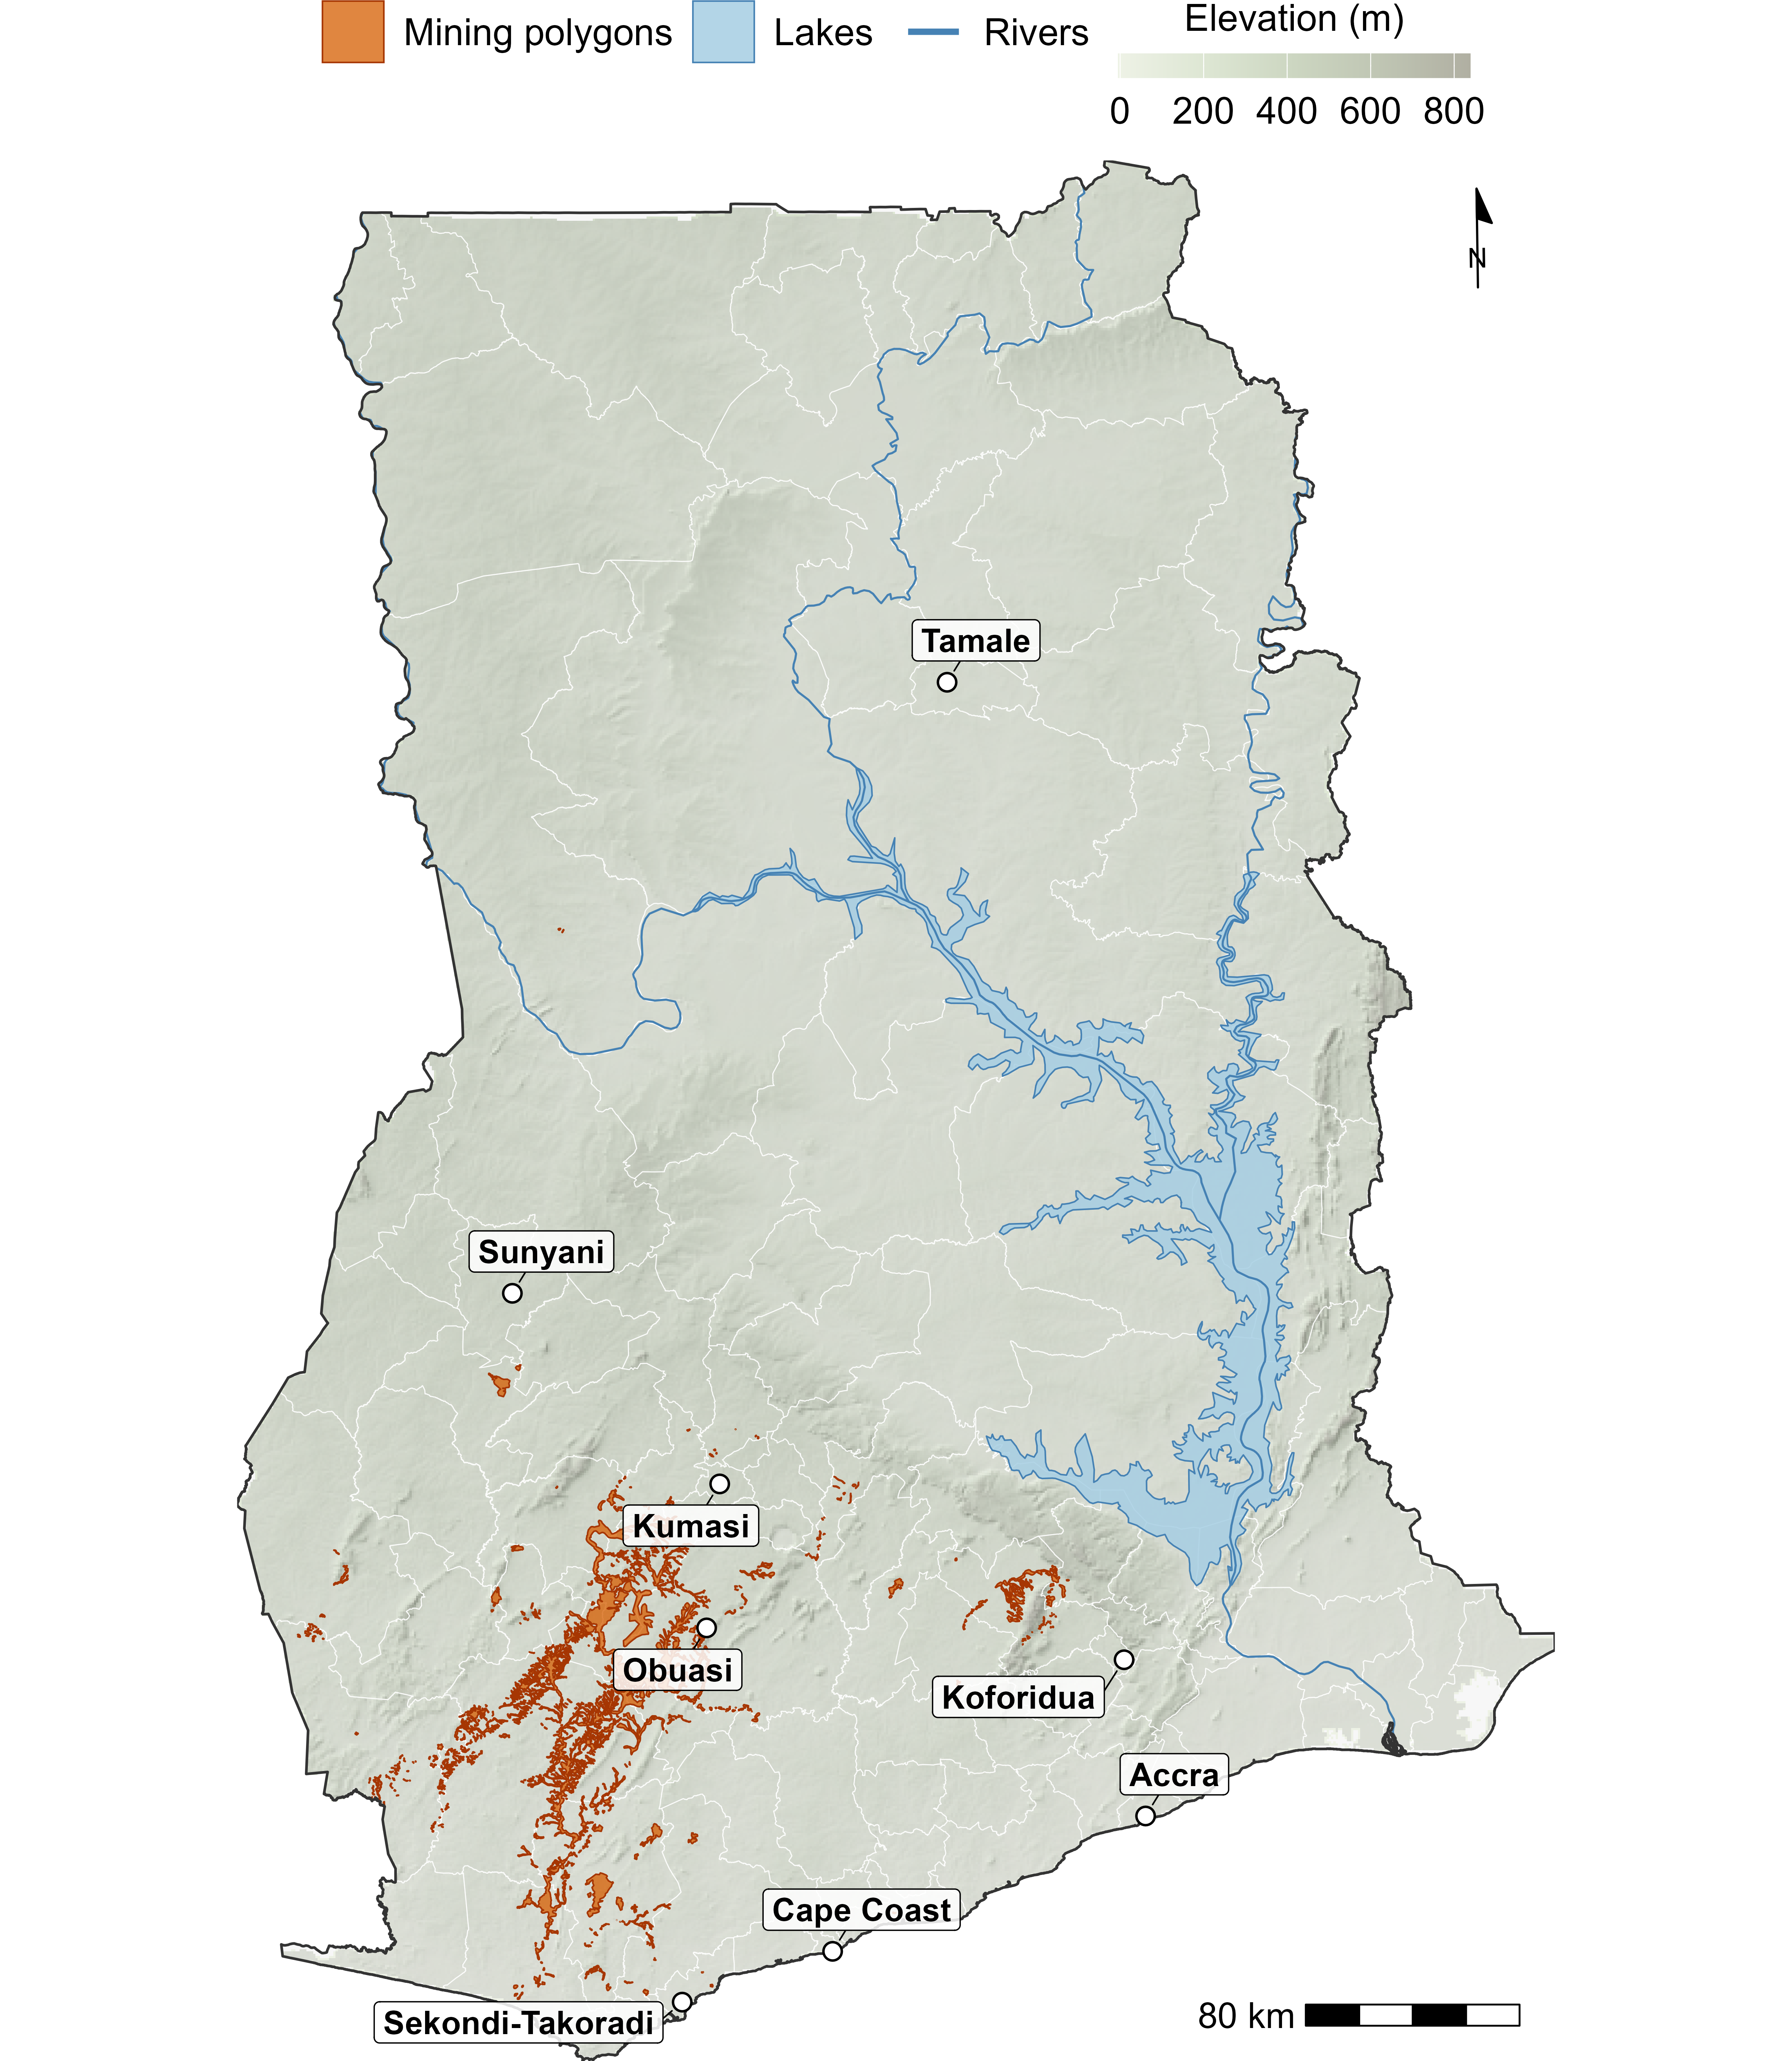
\includegraphics[width=1\textwidth]{figures/fig_study_area.png}
    \caption{Study area showing mining polygons from \citet{maus2022update}. Mining activity is concentrated in southwestern Ghana. Ghana's districts, elevation, and water overlayed.}
    \label{fig:study_area}
\end{figure}

\section{Methods and Data}
Especially challenging for the creation of consistent time series data across differing sensors (Landsat-Sentinel etc.) is the data quality, resolution, and availability of imagery, impacting choice of methods such as random forest (RF) classifiers or deep learning approaches such as a U-Net or standard Convolutional Neural Network (CNN). \citet[pp.170,172]{ma2019Deep}, \citet{ball2017Comprehensive}, and \citet[p.25]{kattenborn2021Review} point out that RF perform well with few training samples, while deep learning approaches require finer resolution imagery (10~m or lower) and detailed training data to learn mining features appropriately but handle feature engineering and variables implicitly. \citet[pp.7-9]{nursamsi2024Remote} showcase that in areas of high spectral confusion such as polluted water bodies and forest mining sites, pixel based RF can produce high accuracy classification, although country context and sensor type are decicive for the choice of method.

The publication of global mining polygons by \citet{maus2020globalscale,maus2022update} introduced manually digitized and verified mining polygons for 2019, improving on previous mining datasets derived from concession boundaries or point locations \citep{maus2022update}. The dataset also captures both industrial and artisanal operations, providing unprecedented reference data for temporal analyses. \citet{maus2022update} mining data enables both the focused sampling of datapoints and the training of classification models using the historical Landsat acrchive\footnote{Longest continuous and publicly available record of medium-resolution multispectral imagery, enabling retrospective analysis of land cover change at regional and global scale \citep{potapov2022Global,roy2016Characterization}.} through Google Earth Engine's cloud computing platform \citep{gorelick2017Google}. Since random forest classifiers show good robustness to noise, low data quality, ability to handle spectral information of diverse landscapes, and resistance to overfitting \citep{belgiu2016Random,rodriguez-galiano2012assessment,gislason2006Random,breiman2001Random,phiri2017Developments}, I decided to train an ensemble of RF classifiers for my historical time-series analyses. 

As my study period covers coarse resolution (30m) years with low data quality, and spans multiple sensor shifts, my study opts for a RF approach over deep learning as they require rich training data and high resolution imagery which is only available in more recent years \citep{kattenborn2021Review,nursamsi2024Remote,gallwey2020Sentinel2}. I validate my mining onset results against a CNN for comparison.

\subsection{Satellite imagery and composite generation}
For my analysis, I created a time series of cloud-masked satellite composites spanning 2000 to 2019 at 30~m resolution using Google Earth Engine \citep{gorelick2017Google}\footnote{The highest possible resolution available for free and for the entire study period.}. Since surface reflectance signatures vary significantly between wet and dry seasons in Ghana \citep{flood2013Seasonal}, I restricted image aquisition to the extended dry season (November through April) to ensure spectral consistency across years.

To address persistent cloud contamination in Ghana's South-West \citep{barenblitt2021large}, I opted for medoid compositing within three-year temporal windows centered on each target year to maximize cloud-free coverage while maintaining spectral consistency \citep{phan2020Land,flood2013Seasonal}.

\subsection{Variables and feature selection}
Each composite was created with 40 bands initially, including six categories of bands, plus quality control bands (See Table~\ref{tab:variables}). Spectral bands, spectral indices, water indices, urban index, and topographic bands information was used as specified by the latest literature. After dropping quality (``housekeeping'') bands, I used all 27 remaining bands for training of the random forest classifier. For validation, I conducted a comprehensive feature analysis, comparing data- and literature-driven selection for the national model (See appendix C for full data report).

\subsection{Training data collection}
To train the classifier on the Landsat composite, I sampled and validated 1409 training points manually using the 2019 composite as a reference layer in GEE \citep{gorelick2017Google}, with NDVI, RGB, and BSI for visual interpretation. I orginally sampled from seven landcover classes (bare soil, water, dense forest, shrubland, flooded vegetation, cropland, built-up) according to ESA World Cover \citep{zanaga2021ESA} data layer before aggregating to three target classes for classification: Water (including tailings ponds), Mining (bare soil, built-up), and Vegetation (cropland, dense forest, shrubland, flooded vegetation). This classification scheme is appropriate given my focus on mining expansion within known mining areas, where the primary distinction is between converted (mining-related) and unconverted (vegetation) land cover. I sampled stratified across three buffers, inside and around (1-2~km; 2-5~km) the \citet{maus2022update} mining poplygons to ensure spectral representation \citep[p.~388]{duckham2024GIS}. Underrepresented classes (Like water around northern mining sites) were sampled across the wider ecological zones, leaving minimum one kilometer around training points to ensure spatial represenation\footnote{Note that some training points are naturally clustered at less than 1~km, like mining points inside concessions.}.

\subsection{Random forest classification}
I trained one national ensemble random forest model for my study area using all training points and the \texttt{ranger} package in R \citep{wright2017Ranger}\footnote{See Appendix C~2 for modelling choices and tests across ecologically diverse areas.}. Following recommendations by \citet{belgiu2016Random} and \citet{svoboda2022Random}, the ensemble comprised five models with 500 trees each. I followed hyperparameter recommendations by \citet{gislason2006Random} using a sample fraction of 0.6 in each RF tree for bootstrap diversity. In addition to the classification raster, I also saved the class probability rasters for validation (simulations).

Class imbalance was addressed using square-root inverse-frequence class weights as \citet{buda2018systematic} specify. The mining class typically represented 15 to 25\% of training samples depending on zone, with vegetation dominating in forest areas and water being the minority class throughout.

For validation of accuracy, I report a full national confusion matrix per class, computing overall accuracy, as well as precision and recall curves with per class and zone F1 scores \citep{olofsson2014Good,tharwat2020Classification,stehman2019Key}. 

\subsection{Transition constraints}
I trained my ensemble model on the full Ghana 2019 composite and classified landcover backward to earlier years (2000 through 2018), generating probability scenarios for each class at national and district level. Since this ``unconstrained'' time series from the majority ensemble vote allows for any landcover transition between years, I then apply `temporal transition rules' on the unconstrained classification rasters so that going back in time, pixels classified as Bare/Mining or Water in 2019 can only transition to Vegetation in earlier years, never vice versa. This enforces the ecological assumption that mining area is increasing and that vegetation does not instantaneously regenerate after mining disturbance. This assumption is reasonable for my study period given that: (a) mining expansion in Ghana has been broadly increasing since 2000 \citep{mcquilken2016Artisanal,aikins2024Ghana,asori2022illegal}; (b) active transformation of mining land to vegetation is rare and slow \citep{barenblitt2021large}; and (c) the 2019 polygons capture currently active operations, not historical, abandoned mines.

I treat the transition-constrained approach as the primary method for quantifying mining expansion, as it prevents ecologically implausible transitions (e.g., dense forest appearing one year after active mining) that can arise from inter-annual classification errors, especially considering the poor image-quality in earlier Landsat years (Pre-2013). I assess the transition rules by extracting class probabilities for N=1000 simulations of Ghana's mining expansion per pixel over time and comparing confidence intervals. I display and discuss the district level and national mining area estimates for my study period. To assess whether my contraint approach is too restrictive I compare mining onset for major industrial operations from industry statistics and a CNN (See appendix E and F).

\subsection{Mining area quantification}
Classified output rasters were spatially intersected with Ghana district boundaries from the Integrated Public Use Microdata Series \citep{ruggles2025Integrated} to generate both national and district-level mining area statistics. Within the mining polygon boundaries of \citet{maus2022update}, I report:

\begin{itemize}
    \item Total mining-related area (Bare/Mining + Water classes) within the mining polygons in ha, both on national and top five district level
    \item Year-over-year change in mining area nationally and per top 5 districts
\end{itemize}

By constraining analysis to the validated mining polygons, my approach captures comprehensive mining impacts including infrastructure, tailings, and cleared areas development that previous studies may have classified as non-mining land cover \citep{barenblitt2021large}. Mining activities that occurred outside the mining polygons of \citet{maus2022update}, under tree canopy, or operations that have been abandoned will not be detected by my approach. However, given the increasing gold prices and intensification of mining in Ghana, my assumption of expanding mines should hold true and contribute with relevant estimates. 

\section{Results}
\subsection{Mining expansion trends}
Mining operations in Ghana, including different resources and types of operations (E.g. Large-scale industrial, small-scale artisanal etc.) expanded from 1\,623~ha in 2000 to 53\,391~ha in 2019, a gradual increase over my study period (Figure~\ref{fig:mining_expansion_curve}). Three broad expansion phases are visible in my time series data (See Fig.~\ref{fig:mining_expansion_curve} below and Tab.~\ref{tab:mining_footprint_temporal} under appendix B). Between 2000 and 2010, mining activities expanded steadily, as they remained concentrated around established industrial mines at Tarkwa and Damang, with Kenyasi industrial mine leaving a significant impact on the numbers once operational in 2005. A significant acceleration then began in 2012, with annual additions of 4\,035~ha (2012),  and 5\,674~ha (2013), representing a steep increase in land conversion to mining. This surge coincides with the peak of the global gold price and the widely documented influx of thousands of miners to Ghana's mining areas to take up mechanised artisanal mining. Growth then slowed temporarily in 2014 (2\,369~ha) before resuming at an intensified pace from 2016 onward. 2017 through 2019, my study period's final years, stand out as statistically unusual, with $z$-scores of 1.69 (2017), 1.55 (2018) and 1.59 (2019), showing annual expansion rates well above the 20-year statistical average. These years collectively added over 20\,667~ha of newly converted land within the mining areas.

\begin{figure}[H]
    \centering
    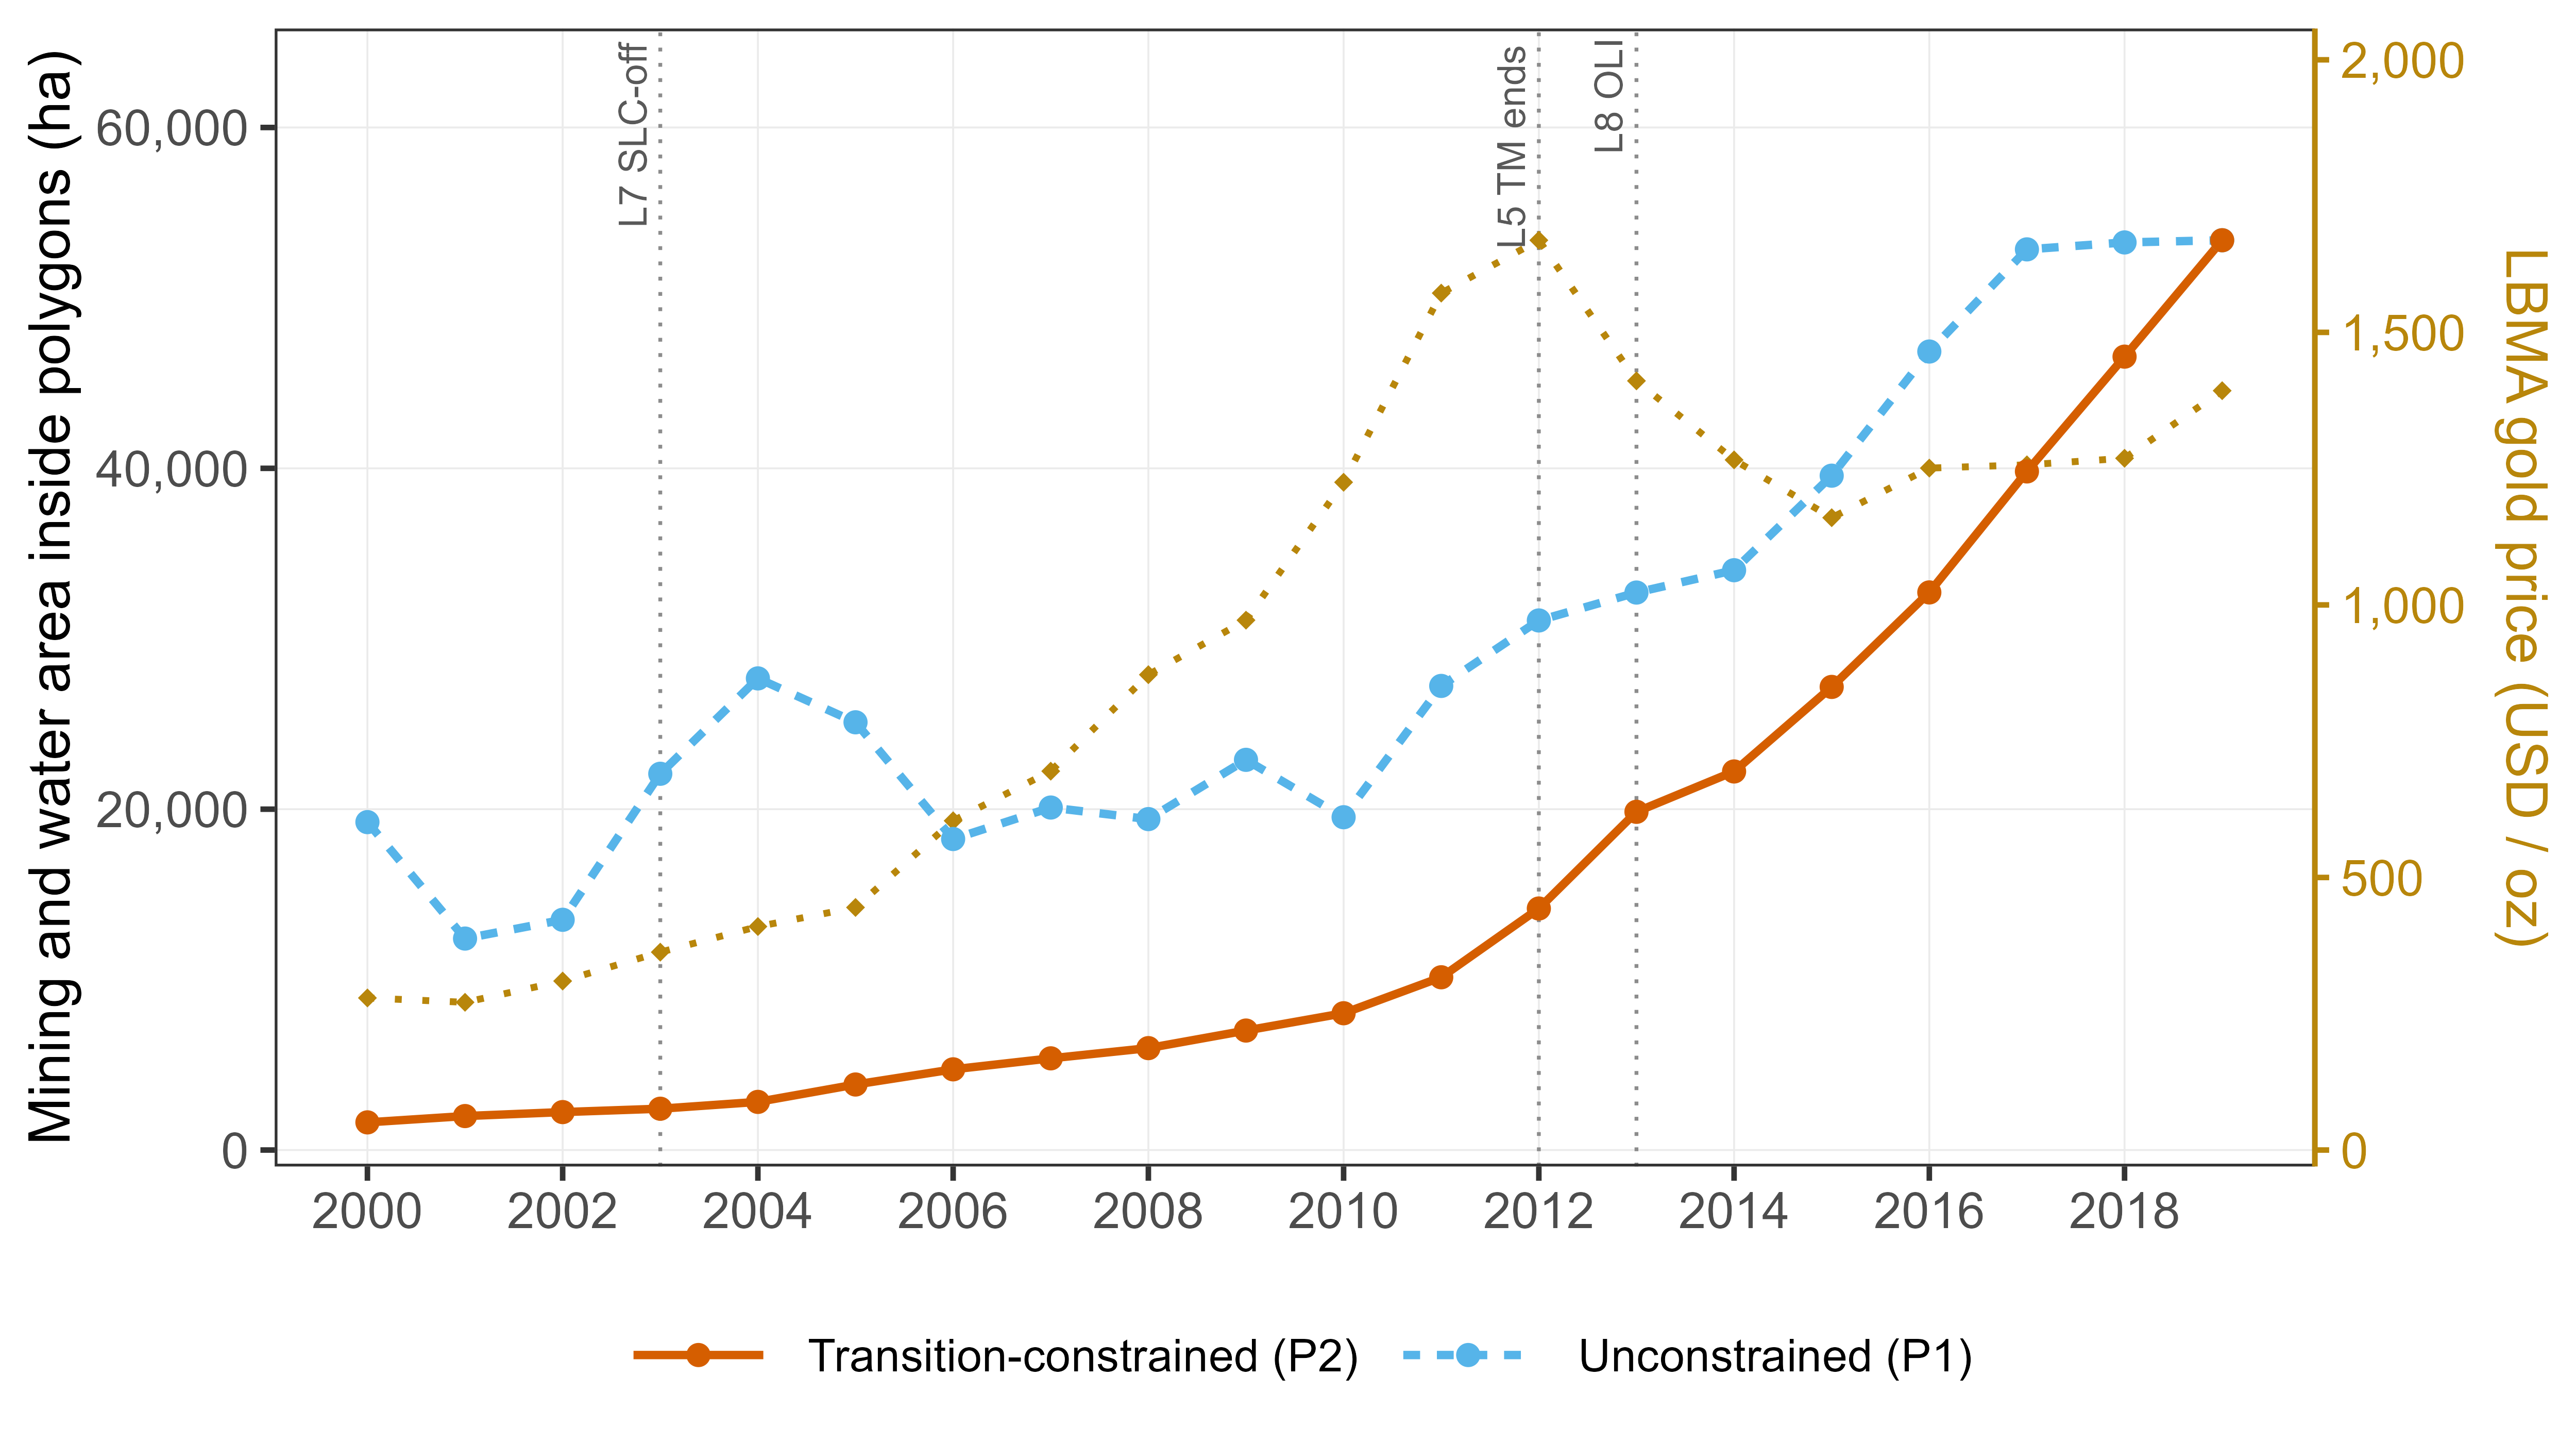
\includegraphics[width=0.9\textwidth]{figures/fig_constraint_vs_gold.png}
    \caption{Comparison of unconstrained (blue) and constrained (red) classification results for 2000 to 2019. Gold price (USD) overlayed. Sensor eras indicated.}
    \label{fig:mining_expansion_curve}
\end{figure}

\begin{figure}[H]
    \centering
    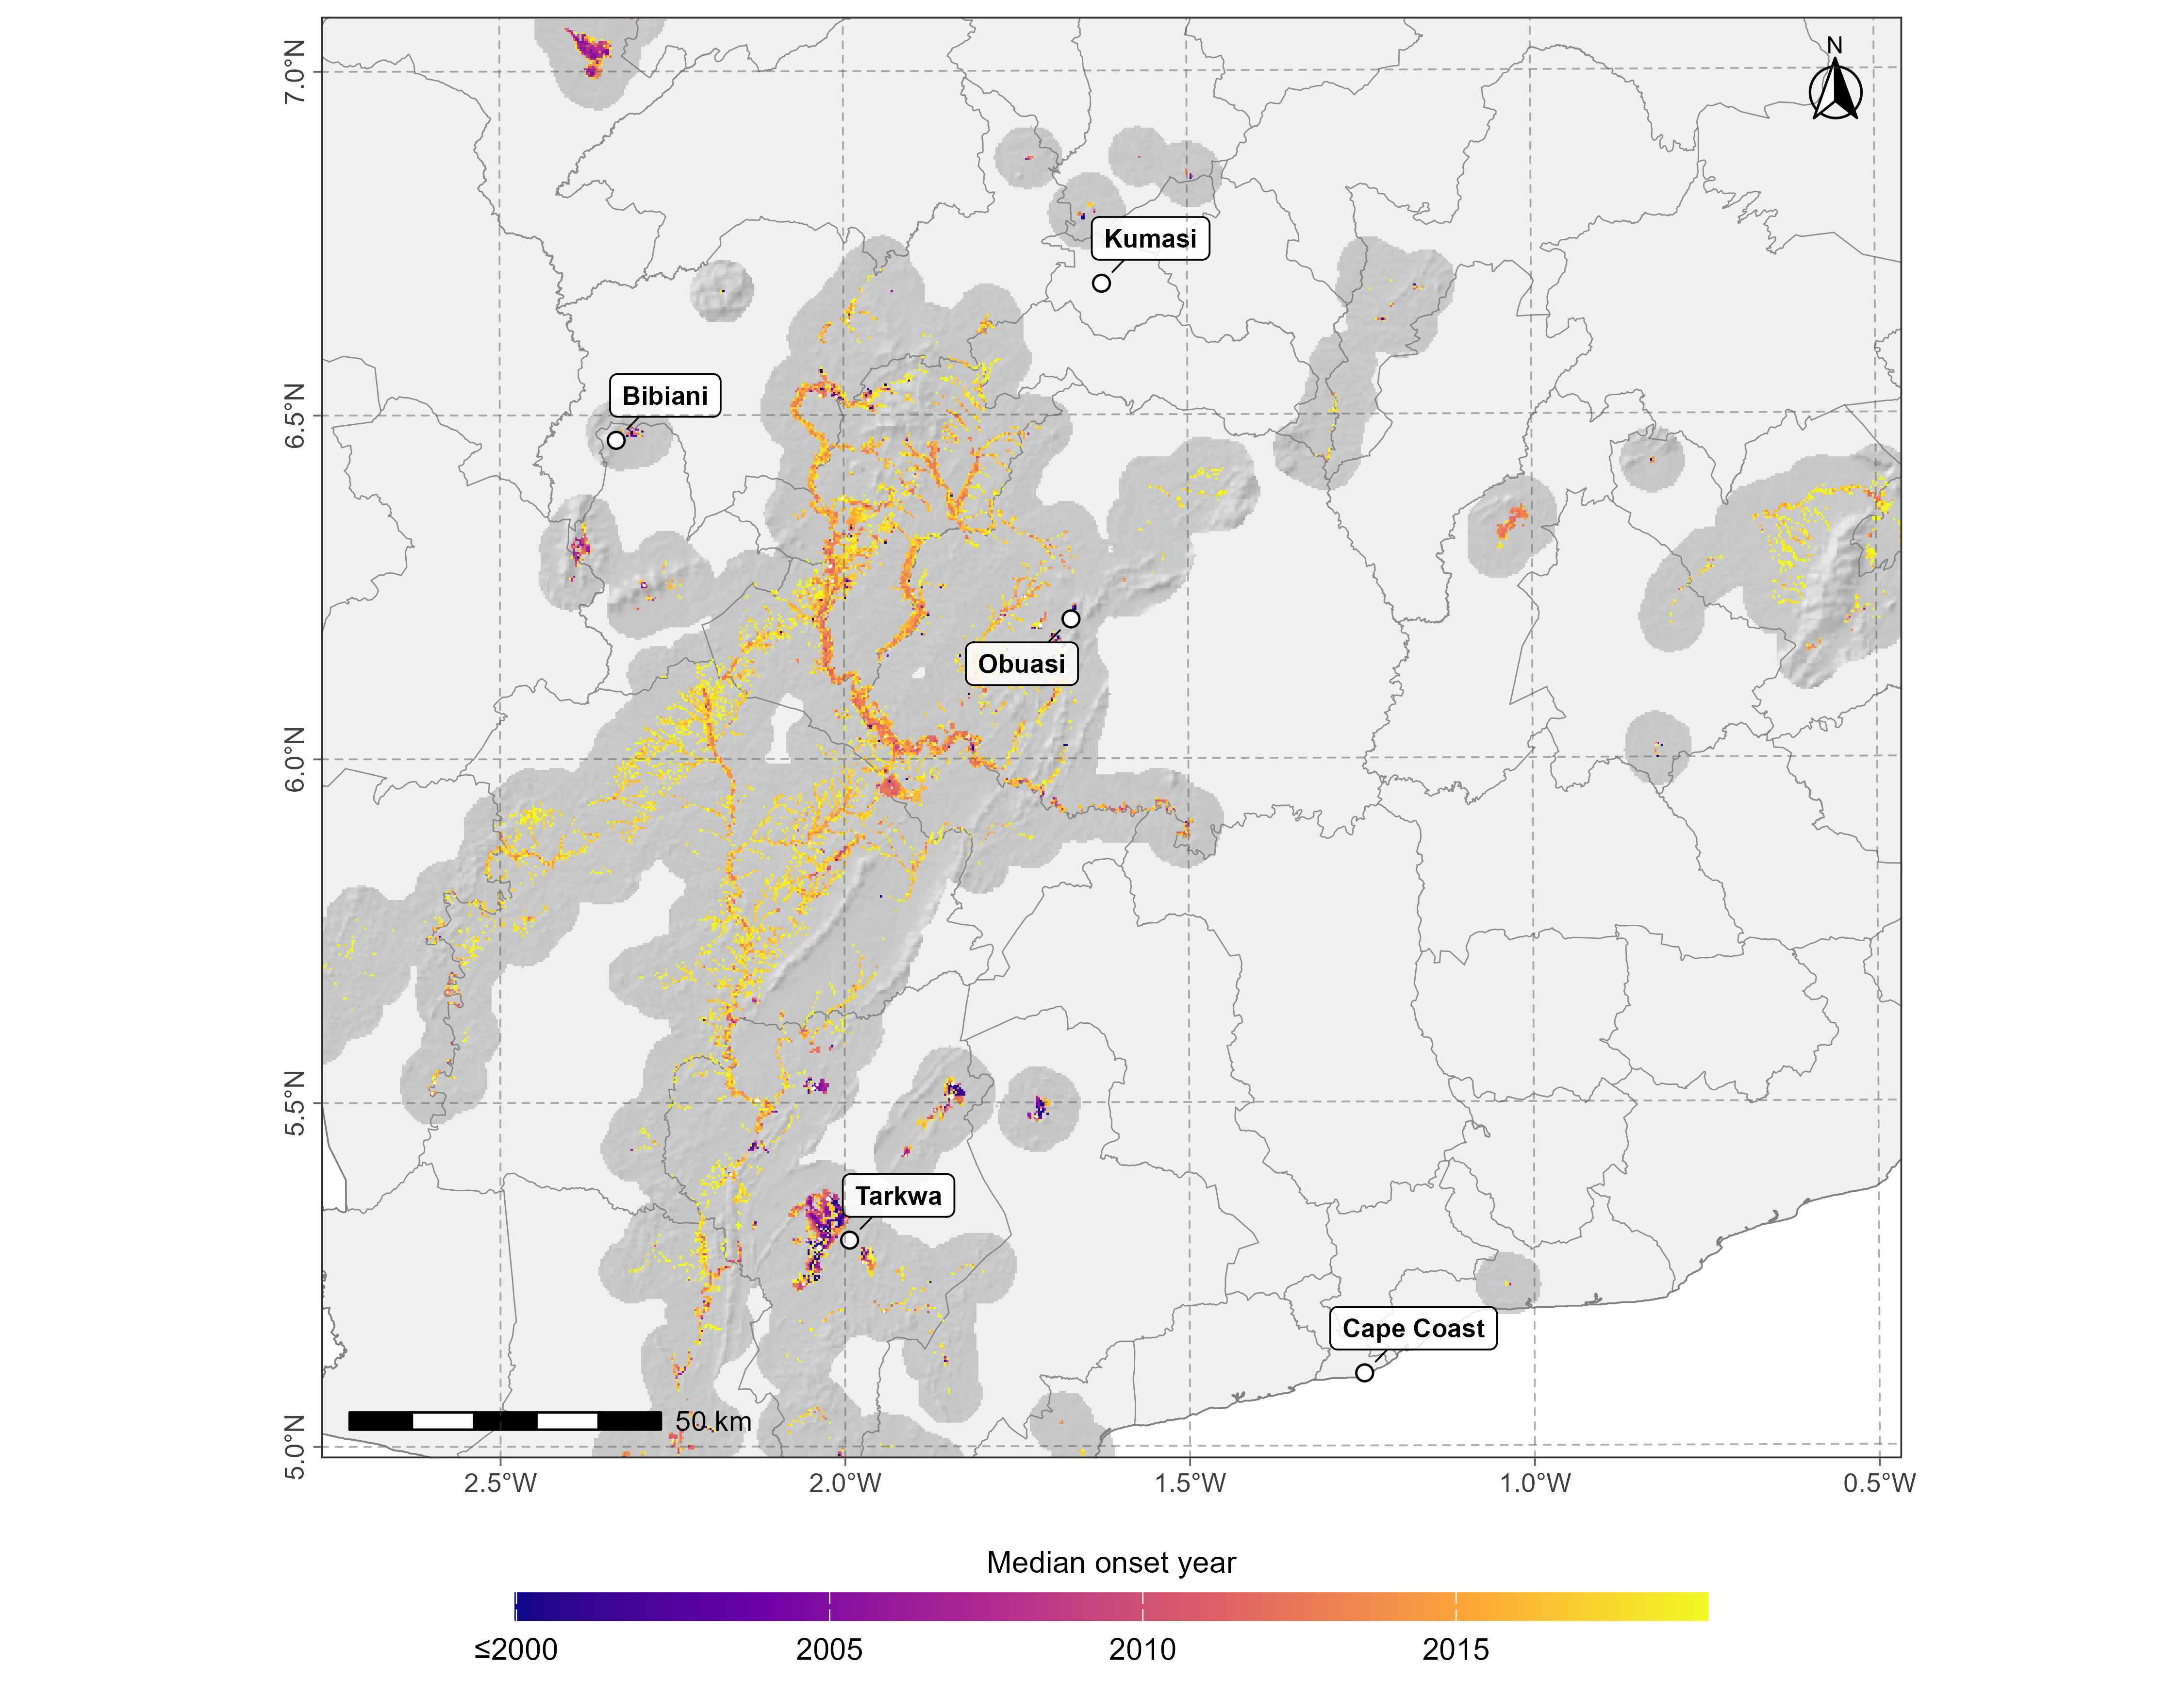
\includegraphics[width=1.0\textwidth]{figures/fig_onset_map.png}
    \caption{Mining onset across study area (\citet{maus2022update} polygons plus 5~km buffer).}
    \label{fig:fig_onset}
\end{figure}

Mining expansion was also concentrated geographically. Five districts make up the majority of Ghana's mining footprint: Tarkwa Nsuaem, Amansie West, Wassa Amenfi, Upper Denkyira, and Asutifi (Table~\ref{tab:district_tarkwa}, Table~\ref{tab:district_amansie}, Table~\ref{tab:district_wassa}, Table~\ref{tab:district_denkyira}, Table~\ref{tab:district_asutifi} in Appendix.). Each of the districts shows unique expansion patterns reflecting local mining histories. For example Tarkwa Nsuaem is home to Ghana's largest open-pit gold operation and showed the most steady growth trajectory, expanding from 783~ha in 2000 to 8\,149~ha in 2019. Expansion was gradual throughout the first decade, before accelerating sharply after 2016, with 2019 alone adding over 723~ha. This increase reflects not just mining intensification within established concessions, but also increased small-scale operations around industrial mining sites.

Amansie West experienced an abrupt single-year increase from 1\,820~ha in 2012 to 3\,854~ha in 2013 ($z = 2.14$), adding 2\,033~ha in a single year likely due to the influx of up to 50,000 national and international miners \citep{aikins2024Ghana,asiedu2023Assessing} and the beginning of the establishement of Asanko mine (not to be openend before 2016 though). In Wassa Amenfi, mining area remained below 1\,000~ha until 2012, then grew rapidly to 11\,657~ha by 2019. The years 2017 to 2019 showed the largest expansion of any district and year combination in this analysis ($z = 1.97$, 2.31, and 1.76), with annual additions exceeding 2\,000 to 2\,500~ha. This pattern is consistent with the rapid expansion of artisanal mining into previously forested concession areas in the Western Region \citep{asiedu2023Assessing,asori2022illegal}, which now threaten food security, and environmental health \citep{barenblitt2021large,mensah2015Environmental,mensah2025Subaltern}.

Upper Denkyira followed a broadly similar path but at smaller scale, growing from 68~ha to 6\,343~ha. Its earliest significant expansion occurred in 2013 ($z = 1.85$), with a hightened intensification visible after 2015. Lastly, Asutifi district stands out as its expansion was dominated by a single event in 2005 ($z = 2.55$), when the Newmont Ahafo mine became operational. The mining surface expanded from 13~ha to 381~ha (2005) and then 660~ha (2006) following the establishment of the mine before growth stabilised at a modest 107~ha/yr average for the remainder of the study period.

\subsection{Classification accuracy}
For my national model (2019), spatial cross-validation showed an overall accuracy of 0.87, with an overall kappa {\textbf{$\kappa$}} of 0.80 (Table~\ref{tab:model_performance} below). The model generally classified well across Ghana's diverse landscape, though a few things stand out. Mining detection in Ghana's North was challenging for the model (Mining F1=0.56), whilst water detection was best across the study area. This indicates an effect of the few available mining training points in the zone but also points to strong spectral contrast between water and vegetation in Ghana's north. The Forest Transition zone performed very well (0.88), whilst the Coastal zone (0.88) showed best seperation of the mining class (F1=0.83) despite being prone to coastal haze and heterogenous landscapes. Most confusion occurred between mining and vegetation, especially in the north, pointing towards the sparesly vegetated landscape there.

\begin{table*}[htbp]
\centering
\caption{2019 national RF model performance under spatially blocked 5-fold cross-validation. Buffer distance of 2.2\,km derived from empirical variogram (See section~3.5). Zone rows split by ecological zone; the model itself does not use zones.}
\label{tab:model_performance}
\small
\begin{threeparttable}
\begin{tabular}{lccccccc}
\toprule
\multirow{2}{*}{\textbf{Scope}} & \multirow{2}{*}{\textbf{n}} & \multirow{2}{*}{\textbf{Accuracy}} & \multirow{2}{*}{\textbf{95\% CI}} & \multirow{2}{*}{\textbf{$\kappa$}} & \multicolumn{3}{c}{\textbf{Per-class F1}} \\
\cmidrule(lr){6-8}
 & & & & & Water & Mining\textsuperscript{b} & Veg. \\
\midrule
\textbf{National}                    & \textbf{1\,394} & \textbf{0.87 $\pm$ 0.03} & \textbf{[.83,\,.91]} & \textbf{0.80} & \textbf{0.93} & \textbf{0.78} & \textbf{0.88} \\
\midrule
\multicolumn{8}{l}{\textit{By latitude zone (same out-of-fold predictions)}} \\
Northern Savannah\textsuperscript{a} & 361   & 0.88 $\pm$ 0.06 & [.80,\,.95] & 0.80 & 1.00 & 0.56 & 0.87 \\
Forest-Transition                    & 519   & 0.88 $\pm$ 0.07 & [.79,\,.96] & 0.80 & 0.92 & 0.82 & 0.89 \\
Coastal                              & 514   & 0.88 $\pm$ 0.05 & [.82,\,.94] & 0.81 & 0.89 & 0.83 & 0.90 \\
\bottomrule
\end{tabular}
\begin{tablenotes}[flushleft]
\footnotesize
\item Accuracies are mean $\pm$ SD across the 5 spatial folds; 95\% CIs are t-distribution intervals across folds. F1 and Cohen's Kappa ($\kappa$) are fold means. Training data: 367 water, 391 mining and 636 vegetation samples (15 of 1\,409 points dropped for missing band values). One-vs-rest AUC (national): water 0.99, mining 0.91, vegetation 0.95.
\item[\textsuperscript{a}] Northern Savannah training data: 146 water, 46 mining and 169 vegetation samples. Only one mining site falls into the northern zone, so samples are few, making the zone estimate honest and more uncertain.
\item[\textsuperscript{b}] Northern zone characteristics drag down overall F1 mining, but model predicts well in the major mining areas.
\end{tablenotes}
\end{threeparttable}
\end{table*}

The achieved overall mining class F1-score (0.78) indicates good balance between precision and recall for the primary class of interest in most parts of my study area (South-Western Ghana (Forest transition and Coastal zones)). Systematic comparison of my national model vis-á-vis zone specific ones, with zone-specific features revealed that they perform similarily under identical conditions (See appendix~\ref{tab:benchmark_master} for full model performance assessment).

My results were also insensitive to the CV design with accuracy varying by less than 0.3 points for buffers of 0 to 10\,km (the fitted variogram range is 0.2 to 6\,km) and block sizes of 10 to 100\,km. Random CV was only 0.7 to 0.9 points more optimistic, and the median test-to-training distance in my spatial CV (12.5\,km) exceeded that of mapped pixels inside the mining polygons (3.3\,km)\footnote{See also Appendix C2 and Fig.~\ref{fig:areaofa} for spatial assessment of cross-validation.}.

\section{Discussion}
\subsection{Comparison with existing estimates}
My analysis points towards 51\,768~ha of converted land to mining between 2000 (1\,623~ha) and 2019 (53\,391~ha) within known mining polygons, following steep expansion trends after 2012, also observed by other studies \citep{snapir2017Mapping,barenblitt2021large,gallwey2020Sentinel2,obodai2019Land,forkuor2020Mapping}. Therein, my estimates sit between those of \citet{barenblitt2021large} and \citet{gallwey2020Sentinel2}, which both tried to mainly estimate land conversion to small-scale mining (but capture some industrial footprints). Whilst \citet{barenblitt2021large} attempt to map historical \textit{artisanal} mining expansion in Ghana (2007-2019), reporting 47\,414~ha of vegetation converted to mining in Ghana's southwestern forest zone, \citet[p.10]{gallwey2020Sentinel2}, using a CNN on high-resolution imagery (Sentinel at 10m resolution) in recent years (2015-2019), show an increase of total converted land to small-scale mining from 64\,000~ha (2015) to 77\,000~ha (2019). Both studies rely on a study-, or ``catchment,'' area in Ghana's south, creating estimates that exclude Ghana's north, as well as industrial operations and other minerals than gold, which are captured by the \citet{maus2022update} polygons I use. 

Adding to that, my estimates include already operational, earlier mining, as well as small-scale operations outside of the study area of \citet{barenblitt2021large}, \citet{snapir2017Mapping}, \citet{forkuor2020Mapping}, \citet{obodai2019Land}, and \citet{gallwey2020Sentinel2}, rendering my numbers more relevant for all of Ghana and over time (2000-2019). On overall classification accuracy, my model achieves 87\% over 84\% reported by \citet{barenblitt2021large}. I also report spatially blocked cross-validation, uncertainty of the probabilistic estimator, and per-class F1 scores (harmonic mean between precision and recall or ``producer's and user's accuracy'), missing from their validation \citep[p.5]{barenblitt2021large}. In contrast, \citet[pp.10,12]{gallwey2020Sentinel2} show the superiority of deep learning approaches over random forest classifiers in more recent years where high resolution imagery (<10m) is available (3-6 \% higher accuracy), but note that patch classifiers and U-Nets create overestimates by ``smoothing,'' classifying forests, bare surfaces, and river systems (wet sediment and polluted rivers) as mining. Therefore, their estimate should be understood as an upper bound and showcases that deep learning approaches are impractical for estimating expansion in earlier years with coarser resolution imagery (30m Landsat era) as the classifiers require visual context. 

Image quality and availability remains an issue for mining remote sensing, as \citet{barenblitt2021large} had to drop pre-2007 imagery for quality reasons, \citet{forkuor2020Mapping} note that approximately 25\% of Sentinel-1 scenes in their study were unusable due to atmospheric interference, and \citet{gallwey2020Sentinel2} see temporary classification errors during the 2015-2016 El Niño event. Whilst \citet{barenblitt2021large} and \citet{gallwey2020Sentinel2}, amongst others \citep{forkuor2020Mapping,snapir2017Mapping,obodai2019Land}, attempt to distinguish mining from urban land cover, leading to severe class confusion (partly due to data quality, partly due to classifier choices), especially along river systems with wet sediment, I opted for aggregating these classes within known mining polygons, capturing mining infrastructure expansion, too, which their approaches do not detect. Whilst I capture most small-scale and industrial mining, \citet{barenblitt2021large} and \citet{gallwey2020Sentinel2} can capture smaller pockets of mining operations further away from the \citet{maus2022update} polygons but risk more class confusion between bare soil, urban, and actual mining pixels. My approach resolves this confusion by aggregating within the polygons.

Finally, \citet{forkuor2020Mapping} note a slowing of ``artisanal'' mining expansion between 2015/16 and 2018/19 using Sentinel-1 backscatter thresholds, and \citet{gallwey2020Sentinel2} suggest a 6.000~ha redcution in ASM expansion for 2017. My own, and others' estimates \citep{snapir2017Mapping,barenblitt2021large,obodai2019Land} show the opposite trajectory: annual expansion accelerated from 5\,546~ha in 2016 to 7\,100~ha in 2017, with the final three years of my study period pointing to intensification. The divide may be explained by their applied change detection method which captures newly cleared surfaces but may undercount expansion within already-existing mining landscapes \citep{forkuor2020Mapping}, their smaller study areas, data quality, and overcounting of the deep learning classifier \citep{gallwey2020Sentinel2}.

These contrasting findings underscore that methodological choices regarding study period, classification area, class definitions, reference data, sensor type, change detection approach, and temporal constraints can substantially alter conclusions about mining trajectories, and assumptions about the effectiveness of policy interventions. Using the polygons of \citet{maus2022update}, this study contributes a validated annual time series of mining footprints for Ghana from 2000 to 2019, taking temporal and spatial consistency into account, and enabling socio-economic assessments of mining expansions.

\subsection{Effects of temporal constraints}
Especially in the earlier years of my study period, the transition constrains removed a lot of mining area as compared to the unconstrained predictions (Table~\ref{tab:mining_footprint_temporal}). This signals the reality of data availability, quality, and model uncertainty for these years. Without constraints, pixels could be classified as mining in 2005, vegetation in 2006, and mining again in 2007, which reflects an ecologically implausible sequence suggesting poor data quality and difficult classification rather than actual land cover dynamics (This has also been noted by \citet[p. 9]{barenblitt2021large} and \citet[p. 2]{forkuor2020Mapping}). The observed mining expansion in earlier years of the study period corresponds well to qualitative evidence that suggests an intensification of mining activities in the years after new liberalisation laws passed in 2006 \citep{asiedu2023Assessing,asori2022illegal,andrews2018Land}, as well as concession records and production statistics \citep{Industrystatistics}. 

The unconstrained predictions show a significantly higher baseline of mining (19\,244~ha in 2000) within validated polygons (Figure~\ref{fig:mining_expansion_curve})\footnote{See also Table~\ref{tab:mining_footprint_temporal}.} However, the unconctrained expansion trajectory is not linear and cautions against using these numbers: the unconstrained estimates fluctuate between consecutive years, even dropping from 27\,678~ha in 2004 to 18\,252~ha in 2006, and from 22\,899~ha in 2009 to 19\,531~ha in 2010, despite major mines opening during these years (E.g. Kenyasi (2005), Akyem (2013), Asanko (2016)), slow reclamation and long-lasting pollution of mining sites, increased industrialisation of small-scale mining, and an influx of foreign miners \citep{kumah2023Chinese,mensah2025Health}. The literature and qualitative evidence tell a story of increased investments in mining during these years, not less. Fluctuations in the unconstrained area predictions probably reflect poor data quality or genuine class confusion over genuine land-cover reversals (See data quality assessment in appendix D).

To further verify the transition constraints, I extracted class probabilities (N=1000 simulations) across the study period, summing per-pixel class probabilities for mining. This raises the estimated disturbed area inside the polygons from 53\,391 to 68\,061~ha in 2019 (and from 1\,623 to 8\,945~ha in 2000). This is because the many vegetation pixels (vegetation is the majority class throughout) each add a small probability of mining. Since my random forest was trained on a balanced, class-weighted sample (54\% mining and water), its probabilities overstate disturbance where vegetation dominates (See probability-weighted curve in Figure~\ref{fig:det_prob}). I therefore treat this probability-weighted estimate as an upper bound and report the ensemble-argmax numbers as my main results (Fig~\ref{fig:det_prob} and Table~\ref{tab:p3-simulation-diagnostics}).

Lastly, I validated my approach of contraining earlier predictions with mining onset data from the Ghana Minerals Commission \citep{Industrystatistics,Operating}, as well as a trained CNN for major industrial mines (See section 3.7 and appendix Table~\ref{tab:app_cnn_rf_onsets})\citep{nursamsi2024Remote,ma2019Deep,kattenborn2021Review} and looked at mining onset at major small-scale and industrial operations (See Fig~\ref{fig:industrial_mines} and Fig~\ref{fig:fig_4panel}). This allows me to visually interpret my classification rasters for the years of known mining onset and verify against the onset year identified by a CNN, representing deep learning approaches (See appendix Table~\ref{tab:app_cnn_rf_onsets}, Figure~\ref{fig:fig_4panel} and Figure~\ref{fig:fig_onset} below). As expected, the RF does a better job at classifying back in time to the noisy earlier landsat imagery (See Table~\ref{tab:app_cnn_rf_onsets} and Figure~\ref{fig:valid_pixels}) but does not over-restrict pixel-transitions at the same time. Onset years of major industrial mines are captured well, whilst the CNN struggles in earlier years and sees an industrial mine where it only was developed years later. This confirms the insights of the current state of methods, where deep learning approaches rely on good training data and image quality in order to outperform other classification approaches \citep{ma2019Deep,kattenborn2021Review}. RF classifiers on the other hand do well with few training points and perform consistently even in lower-quality data periods.

\begin{figure}[H]
    \centering
    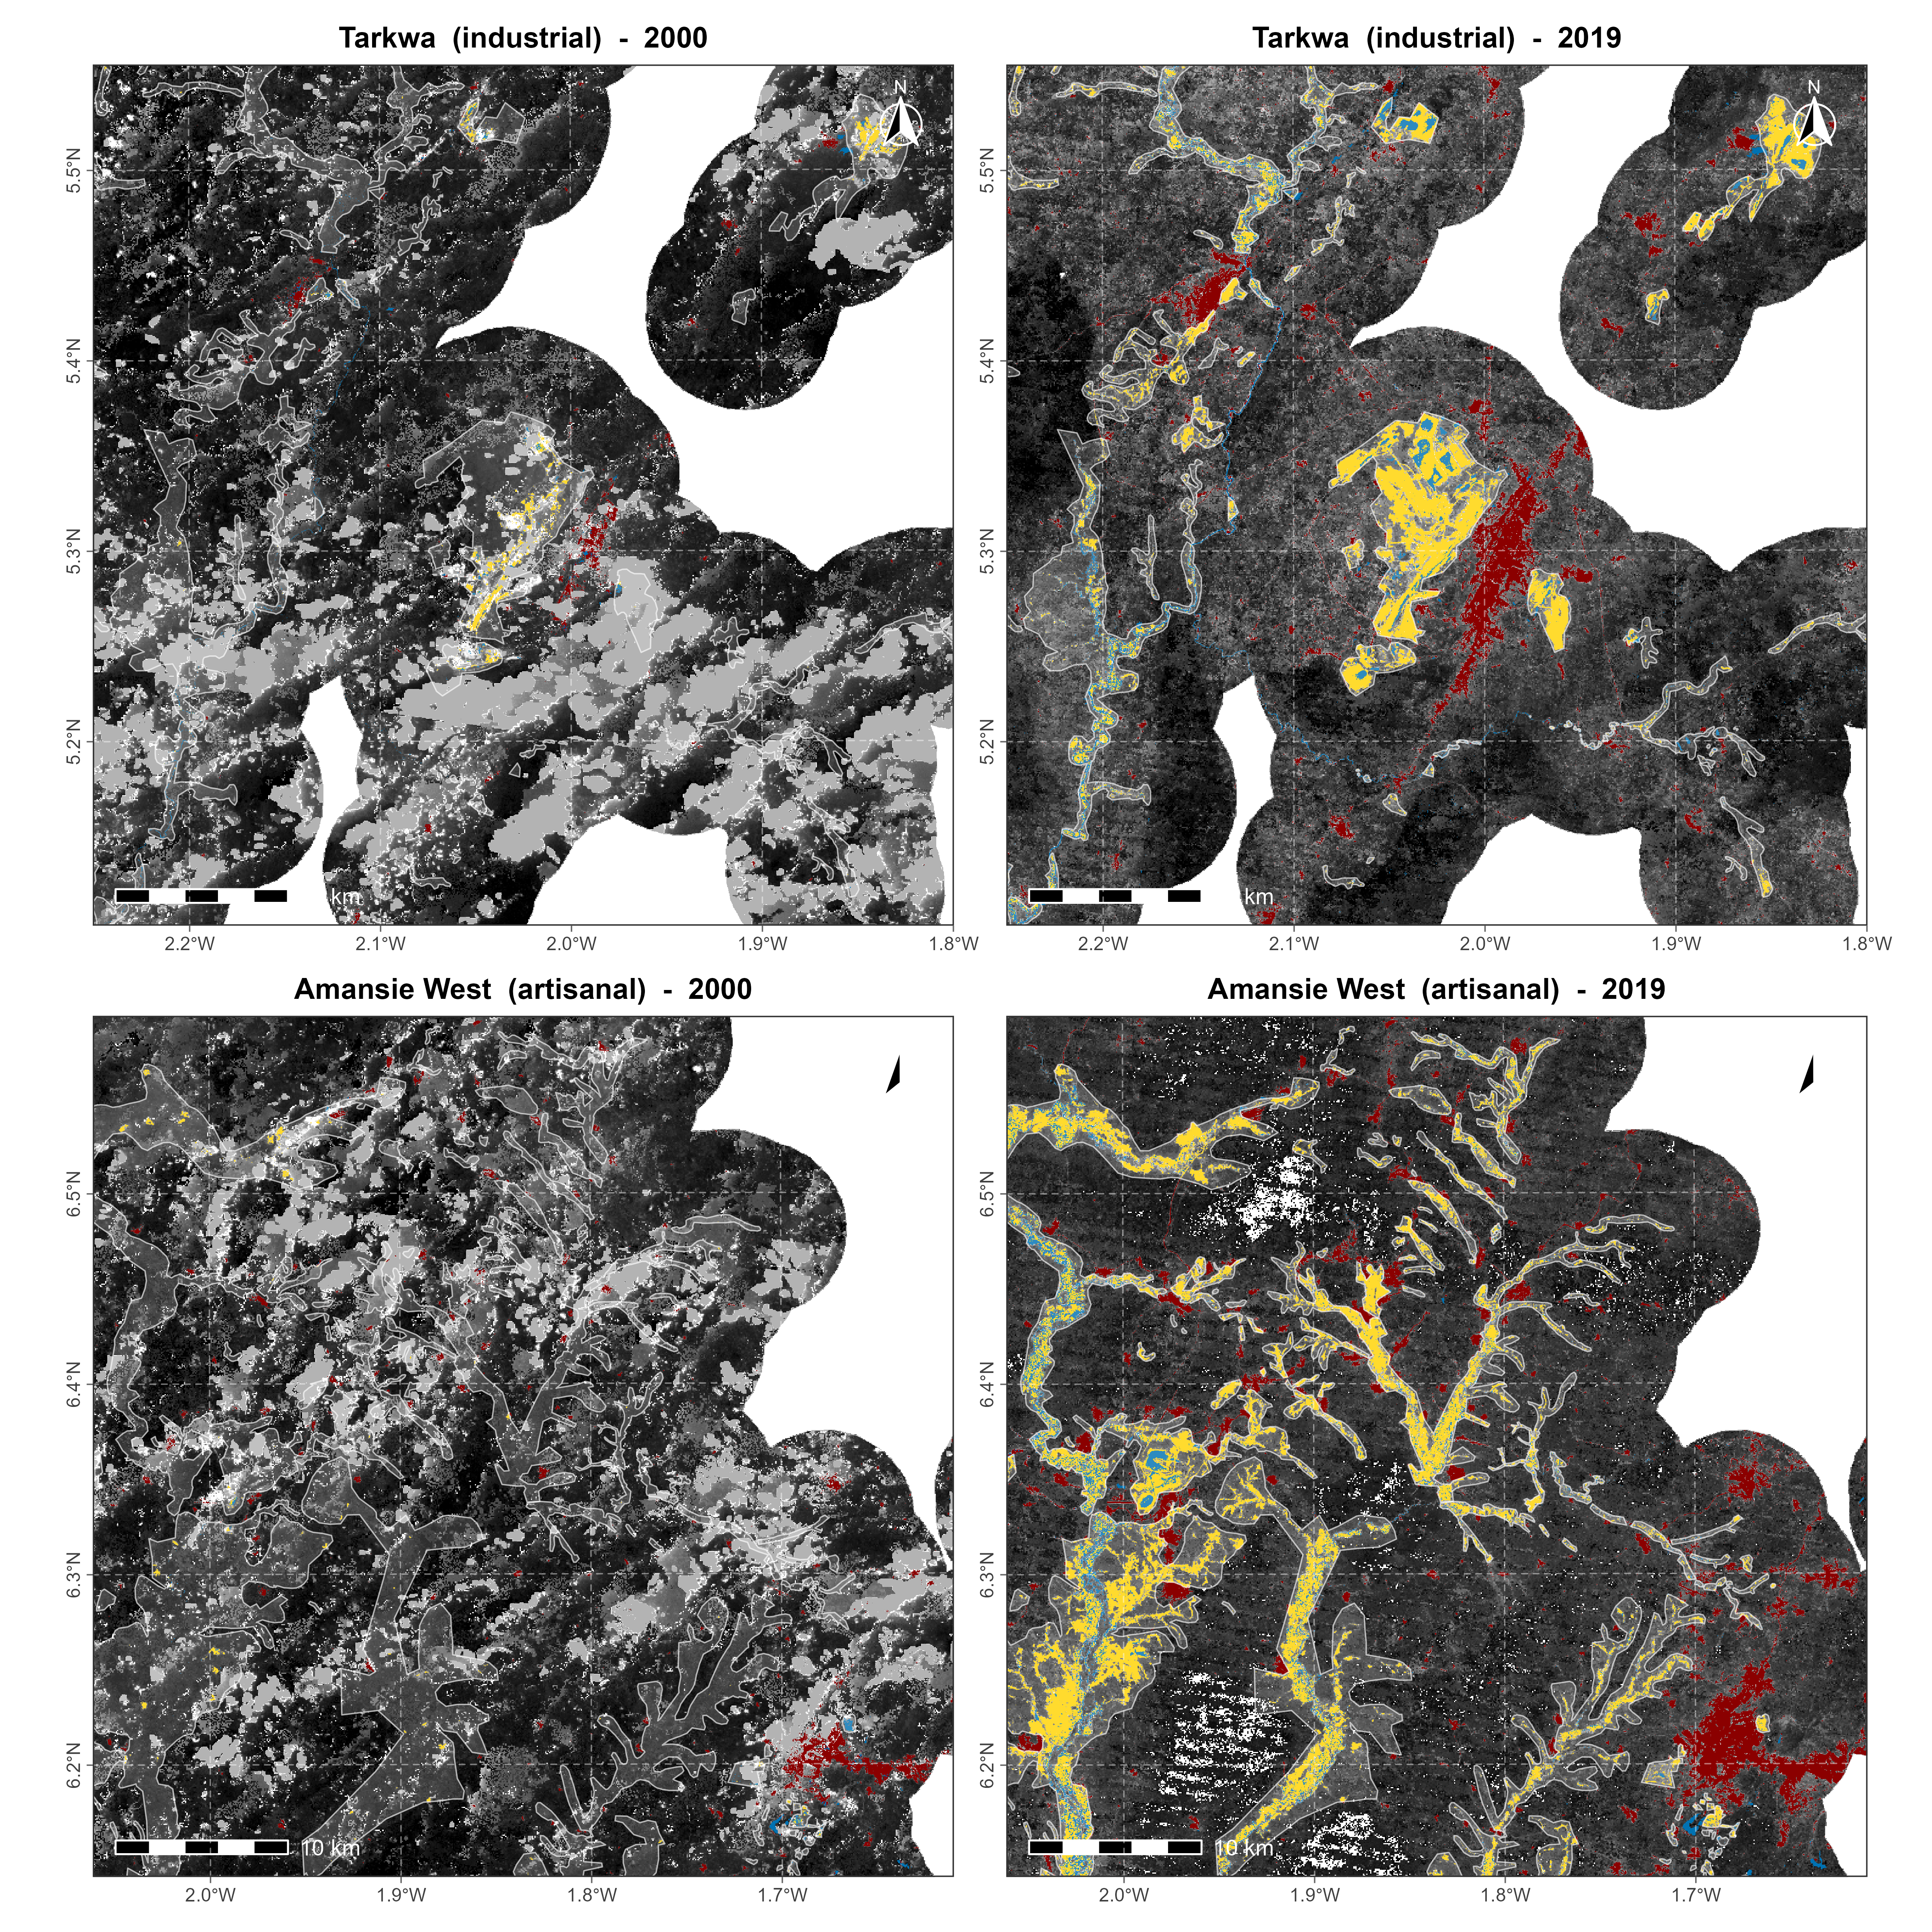
\includegraphics[width=1\textwidth]{figures/fig_overlay_4panel.png}
    \caption{Mining expansion visible at Tarkwa mine and artisanal mining sites close to Obineben. Mining polygons overlayed in transparent white. Mining (water and mining) cells in yellow. NA (cloud pixels) greyed out. Dark red cells outside the mining polygons represent built-up and bare soil, such as towns, streets and other infrastructure.}
    \label{fig:fig_4panel}
\end{figure}

\subsection{Limitations}
In my work I applied quantile-based clipping on my feature bands to constrain outliers (Preserving 99,5\% of valid data), but some inter-annual data quality issues may persist. Composite data quality assessment revealed that early-period predictions (2000–2005) are built on substantially fewer cloud-free observations than later years (See appendix Figure~\ref{fig:valid_pixels}). The 2000 composite averaged fewer than four valid pixels per location across all zones, limiting the medoid algorithm's ability to select a good observation and increasing susceptibility to residual contamination (clouds) and sensor noise. Predictions for these years should therefore be interpreted with greater uncertainty than post-2012 estimates, although mining onset was predicted quite reliably as compared to the trained CNN (See appendix Table~\ref{tab:app_cnn_rf_onsets}). Landsat 8 availability then increased valid pixel counts to 15–30 per composite pixel. Despite these limitations, no compositing method can overcome the fundamental scarcity of cloud-free Landsat observations over tropical West Africa before 2013. The applied medoid approach preserves inter-band spectral relationships better than alternative compositing strategies that risk the `Frankenstein effect' of combining observations from different atmospheric conditions \citep{flood2013Seasonal}. As visible in Figure~\ref{fig:areaofa}, my models predict well across Ghana, but are more uncertain for mining in the north due to the little training data and mining sites located in Ghana's north \citep{maus2022update}. 

My work has focused on estimating the extent and timing of Ghana's mining expansion using remote sensing. Whilst apparently apolitically in nature, I want to echo scholars before me who have noted the `top-down' nature of remote sensing analyses \citep[p.9]{barenblitt2021large}, cautioning against using these methods as a tool to make decision about people without enganging in a deeper dialogue on what the observed changes mean for individuals living in Ghana, taking into account people's perspectives \citep{rutazibwa2023inclusion,lund2013Introduction}.

Whilst the polygons help me produce detailed estimates for Ghana's historical mining expansion at disaggregated level, mining activties outside the 2019 polygon boundaries cannot be assessed. Any mines that were active historically but abanoned before 2019, and some artisanal operations (E.g. under tree canopy) too small to appear in the dataset, can not be captured using my approach. I accept these limitations in my study as Ghana's mining boom is ongoing \citep{asori2022illegal,asiedu2023Assessing,siachiwena2025benefits}, and it can be assumed that even if some mines were abandoned\footnote{See for example \citet{mensah2025Health} on soil remediation and health risks at an ASM site.}, people will either e.g. try to revisit sites with newer equipment, and/or sites won't be usable or transformed until after natural vegetation has regrown from the degraded land. For assessing national and local expansion trajectories within currently active mining areas (2019), my constrained approach is appropriate and produces results that can be linked to population or environmental data for further analysis of mining impacts.

\subsection{Implications for mining impact assessment}
By expanding the definition of the mining landcover class in my study, my approach provides meaningful impact estimates that improve on methods counting mining cells across larger study areas and risk severe class confusion in earlier Landsat years. Tailings ponds, processing facilities, roads, worker housing, and cleared land around mining sites all represent land cover changes with environmental and social consequences \citep{mcquilken2016Artisanal,andrews2018Land} which can be quantified using my suggested approach and the \citet{maus2022update} dataset. Previous studies may have systematically underestimated mining footprints by classifying such infrastructure as urban or bare soil distinct from mining \citep{barenblitt2021large}, or overestimated by risking class confusion between mining, urban, and bare soil \citep{snapir2017Mapping}, or having CNN or U-Net smoothing over mining details in earlier years \citep{ma2019Deep,ball2017Comprehensive,kattenborn2021Review}. Eventhough my expansion estimates are slightly higher than e.g. the ones of \citet{barenblitt2021large}, my numbers are likely underestimates, as areas outside of mining polygons \citet{maus2022update} were not included in this study \citep{gallwey2020Sentinel2}.

The pixel-year based time series data generated by this analysis can support quantitative investigations of mining's relationship with demographic, economic, social, and environmental outcomes when linked to survey or administrative data. My data shows where mining extents expanded most severely (See Fig.~\ref{fig:fig_onset} below), and corresponds well to ground-truth data on industrial mine establishment, and Ghana's artisanal boom from around 2011 \citep{Industrystatistics}. The IPUMS-compatible district boundaries \citep{ruggles2025Integrated} facilitate integration with census microdata for further analyses. For Ghana specifically, my data allows the assessment of policy implications (Such as operation Vanguard targeting artisanal mining \citep{hilson2017Shootings}), and the study of mining impacts on local communities. 

\section{Conclusions}
My analysis demonstrated that polygons of known mining sites can effectively anchor temporal analyses of mining expansion in Ghana. Constraining classification to known mining areas from recent high-resolution footprints, makes possible the assessment of historical mining-related land cover change. This method includes both industrial and ``small-scale'' operations, mining infrastructure, and tailings, contributing meaningful new estimates, especially in a historical perspective and for integration with survey data. My model, achieving overall accuracy of 0.87 shows good applicability across Ghana, vis á vis deep learning methods (CNN), and validated onset information from industry statistics aquired from the Ghana Minerals Commission.

Transition constraints prooved effective in preventing ecologically implausible class dynamics and produce more conservative land cover change estimates as compared to unconstrained classifications. I estimate mining expansion in Ghana from approximately 1\,623~ha in 2000 to 53\,391~ha in 2019, concentrated in southwestern Ghana's forest zone with peak expansion during 2012 to 2013, and from 2016 onward. These findings are in line with qualitative evidence and the establishment of major industrial mines in Ghana's districts.

For Ghana specifically, this study contributes knowledge about the \textit{Where} and \textit{When} of all mining activities from 2000 to 2019 on national and district level, combining industrial and ``artisanal'' for the first time in a time series from 2000-2019. My data shows when and where mining operations began and how they expanded over time. This information is relevant for local populations, researchers, and policymakers to assess how these quantifiable landcover changes coincide with policy shifts (E.g. Operation vanguard, GoldBod) and impacts on humans and the environment.

The methodological framework presented here, using validated polygons as focused classification area, zone-specific model validation, and transition constraints, might be transferable to other mining regions. The global coverage of the \citet{maus2022update} mining polygons suggests broad applicability for historical mining expansion analysis. Besides improving on estimates, these methodos have relevance for ecological realism, and related socio-economic analyses of global mining impacts.

\section*{Acknowledgements}
I would like to thank Jonas Vestby for his continued support and expertise
along the way. Critical comments and ideas by Tone Sommerfelt and the
LANDRESPONSE team led by Tor A. Benjaminsen helped refine this article.
I am also grateful for the input of the Skogrover lunch group at MINA (NMBU).

\section*{Disclosure statement}
No potential conflict of interest was reported by the author.

\section*{Funding}
This work was supported by the European Research Council (ERC) under the
European Union's Horizon Europe research and innovation programme
[LANDRESPONSE, grant agreement number 101054410].

\section*{Data availability statement}
%% GRS requires data AND software to be deposited in a repository that
%% complies with the COPDESS Open + FAIR policies. GitHub alone does not
%% qualify (no persistent identifier); archive a release on Zenodo (or a
%% similar repository) and cite its DOI here.
%% TODO: replace the Zenodo DOI placeholder once the archive is created.
The scripts, training data and replication guidelines that support the
findings of this study are openly available in Zenodo at
\url{https://doi.org/10.5281/zenodo.XXXXXXX} (TODO), with the development
version at \url{https://github.com/hannesbra}.
Landsat imagery was accessed through Google Earth Engine
\citep{gorelick2017Google}. Mining polygons are available from
\citet{maus2022update}. District boundaries can be accessed from
\citet{ruggles2025Integrated}.

\section*{Use of generative AI}
During the preparation of this work the author used Claude Opus 4.7 and 5.5
(Anthropic) to write and streamline Google Earth Engine and R code for producing the
satellite composites and the machine-learning analyses. After using this
tool, the author reviewed, tested and edited the code and its outputs as
needed and takes full responsibility for the content of the publication.

%% =====================================================================
%% REFERENCES (APA via apacite)
%% =====================================================================
\bibliographystyle{apacite}
\bibliography{references} 

\section{Ecological zone descriptions}
\label{app:zones}
As \citet{ploton2020Spatial} and \citet{zhang2026Geographical} show, large-scale ecological mapping models often overestimate their predictive power, and don't take into account locally varying spectral signatures. This is why I divided my study area into three ecological zones with distinct characteristics relevant to mining detection, following the agro-climatic reclassification of \citet{yamba2023Revisiting}. I validate these ecological zones against my national RF model.

Training points were assigned to ecological zones based on latitude thresholds calibrated to balance ecological representativeness\footnote{See training data, and ecological zones in Figure \ref{fig:study_area}.}. Zone boundaries were set at 8.0°N (northern/forest-transition) and 6.0°N (forest-transition/coastal) according to reclassification of \citet{yamba2023Revisiting}.

\textbf{Northern Savannah Zone} ($\geq$8.0°N): Ghana's north receives
unimodal rainfall (ca. 800--1\,200~mm annually) and is mostly sparsely
vegetated. Only one mining site falls into the north. Sparse vegetation helps to detect bare-soil
signatures but also increases spectral confusion between mining and
vegetation classes. Literature-based zone features emphasise BSI and the
SWIR bands.

\textbf{Forest-Transition Zone} (6.0 to 8.0°N): The forest zone has higher,
bimodal rainfall (1\,200 to 1\,800~mm) and consists of dense forest,
plantations and agricultural land. Mining comprises industrial open-pit and underground
operations, and alluvial gold extraction along rivers. Dense vegetation gives
strong contrast to mining, but persistent cloud cover and shadowing
complicate compositing, especially before 2013. Literature-based zone
features emphasise NDVI, MNDWI and texture metrics for detecting canopy
disturbance.

\textbf{Coastal Zone} ($<$6.0°N): The coast has bimodal rainfall with
coastal influences, including mangroves, coastal savannah and intensive
cultivation. Mining includes beach-sand extraction and gold operations in
river deltas. Water indices (MNDWI, AWEI) are expected to be important here.

\section{Annual expansion statistics}
\label{app:annual}

\begin{table}[H]
  \centering
  \small
  \caption{Estimated mining area (ha) inside known polygons
  \citep{maus2022update}, 2000 to 2019. Area combines mining and water class
  pixels within the polygons. Unconstrained area is the per-year argmax
  classification from the national random forest ensemble; constrained area
  applies the transition (shrinking) rule. Annual change and $z$-scores refer
  to the \textbf{constrained} estimates.}
  \label{tab:mining_footprint_temporal}
  \begin{threeparttable}
    \setlength{\tabcolsep}{6pt}
    \begin{tabular}{@{}lrrrr@{}}
      \toprule
      Year & \makecell[r]{Unconstrained\\(ha)} & \makecell[r]{Constrained\\(ha)} & \makecell[r]{Annual\\change (ha)} & $z$-score\tnote{a} \\
      \midrule
      2000 & 19\,244 & 1\,623 & --- & --- \\
      2001 & 12\,410 & 1\,993 & 370 & $-$0.91 \\
      2002 & 13\,511 & 2\,227 & 233 & $-$0.96 \\
      2003 & 22\,081 & 2\,424 & 198 & $-$0.98 \\
      2004 & 27\,678 & 2\,825 & 400 & $-$0.90 \\
      2005 & 25\,102 & 3\,845 & 1\,020 & $-$0.66 \\
      2006 & 18\,252 & 4\,736 & 890 & $-$0.71 \\
      2007 & 20\,099 & 5\,381 & 645 & $-$0.80 \\
      2008 & 19\,421 & 5\,981 & 600 & $-$0.82 \\
      2009 & 22\,899 & 7\,012 & 1\,031 & $-$0.65 \\
      2010 & 19\,531 & 8\,028 & 1\,016 & $-$0.66 \\
      2011 & 27\,236 & 10\,139 & 2\,111 & $-$0.24 \\
      2012 & 31\,078 & 14\,174 & 4\,035 & \phantom{$-$}0.51 \\
      2013 & 32\,716 & 19\,848 & 5\,674 & \phantom{$-$}1.14 \\
      2014 & 34\,027 & 22\,216 & 2\,369 & $-$0.14 \\
      2015 & 39\,575 & 27\,178 & 4\,961 & \phantom{$-$}0.86 \\
      2016 & 46\,860 & 32\,724 & 5\,546 & \phantom{$-$}1.09 \\
      \textbf{2017} & \textbf{52\,855} & \textbf{39\,824} & \textbf{7\,100} & \textbf{\phantom{$-$}1.69} \\
      \textbf{2018} & \textbf{53\,263} & \textbf{46\,560} & \textbf{6\,736} & \textbf{\phantom{$-$}1.55} \\
      \textbf{2019} & \textbf{53\,391} & \textbf{53\,391} & \textbf{6\,831} & \textbf{\phantom{$-$}1.59} \\
      \bottomrule
    \end{tabular}
    \begin{tablenotes}[flushleft]
      \footnotesize
      \item[a] Years with unusually high expansion over the study period's mean ($z > 1.5$) are shown in \textbf{bold}.
    \end{tablenotes}
  \end{threeparttable}
\end{table}

\subsection{Uncertainty validation of the constrained approach}
\label{app:simulation}

\begin{table}[H]
\centering
\small
\caption{Simulation of disturbed area (mining $+$ water) within polygons,
2000 to 2019 ($n = 1\,000$ draws). In each draw one of the five ensemble
members is selected at random for every year; the most likely class is
mapped and the transition rule is applied. Deterministic = constrained map
of the averaged ensemble. PI = empirical prediction interval (2.5th and
97.5th percentiles across draws); relative width = PI width / mean. All
areas in hectares.}
\label{tab:p3-simulation-diagnostics}
\begin{tabular}{@{}rrrrrr@{}}
\toprule
Year & Deterministic & \makecell[r]{Simulation\\mean} & 95\% PI & \makecell[r]{95\% PI\\width} & \makecell[r]{Relative\\width (\%)} \\
\midrule
2000 & 1\,623 & 1\,424 & 1\,332--1\,560 & 228 & 16.0 \\
2001 & 1\,993 & 1\,767 & 1\,651--1\,924 & 273 & 15.4 \\
2002 & 2\,226 & 1\,998 & 1\,867--2\,171 & 304 & 15.2 \\
2003 & 2\,424 & 2\,200 & 2\,050--2\,379 & 330 & 15.0 \\
2004 & 2\,825 & 2\,599 & 2\,399--2\,841 & 442 & 17.0 \\
2005 & 3\,845 & 3\,601 & 3\,335--3\,951 & 616 & 17.1 \\
2006 & 4\,736 & 4\,462 & 4\,200--4\,790 & 591 & 13.2 \\
2007 & 5\,381 & 5\,090 & 4\,830--5\,421 & 591 & 11.6 \\
2008 & 5\,981 & 5\,715 & 5\,406--6\,073 & 667 & 11.7 \\
2009 & 7\,012 & 6\,695 & 6\,380--7\,051 & 671 & 10.0 \\
2010 & 8\,028 & 7\,700 & 7\,366--8\,125 & 759 & 9.9 \\
2011 & 10\,138 & 9\,803 & 9\,326--10\,378 & 1\,052 & 10.7 \\
2012 & 14\,174 & 13\,744 & 13\,043--14\,637 & 1\,594 & 11.6 \\
2013 & 19\,848 & 19\,193 & 18\,320--20\,294 & 1\,974 & 10.3 \\
2014 & 22\,216 & 21\,537 & 20\,512--22\,690 & 2\,178 & 10.1 \\
2015 & 27\,178 & 26\,425 & 25\,129--27\,951 & 2\,823 & 10.7 \\
2016 & 32\,724 & 31\,984 & 30\,307--34\,121 & 3\,814 & 11.9 \\
2017 & 39\,824 & 39\,062 & 36\,869--41\,713 & 4\,844 & 12.4 \\
2018 & 46\,560 & 45\,888 & 43\,146--50\,307 & 7\,161 & 15.6 \\
2019 & 53\,392 & 53\,732 & 50\,263--57\,163 & 6\,900 & 12.8 \\
\bottomrule
\end{tabular}
\end{table}

\begin{figure}[H]
  \centering
  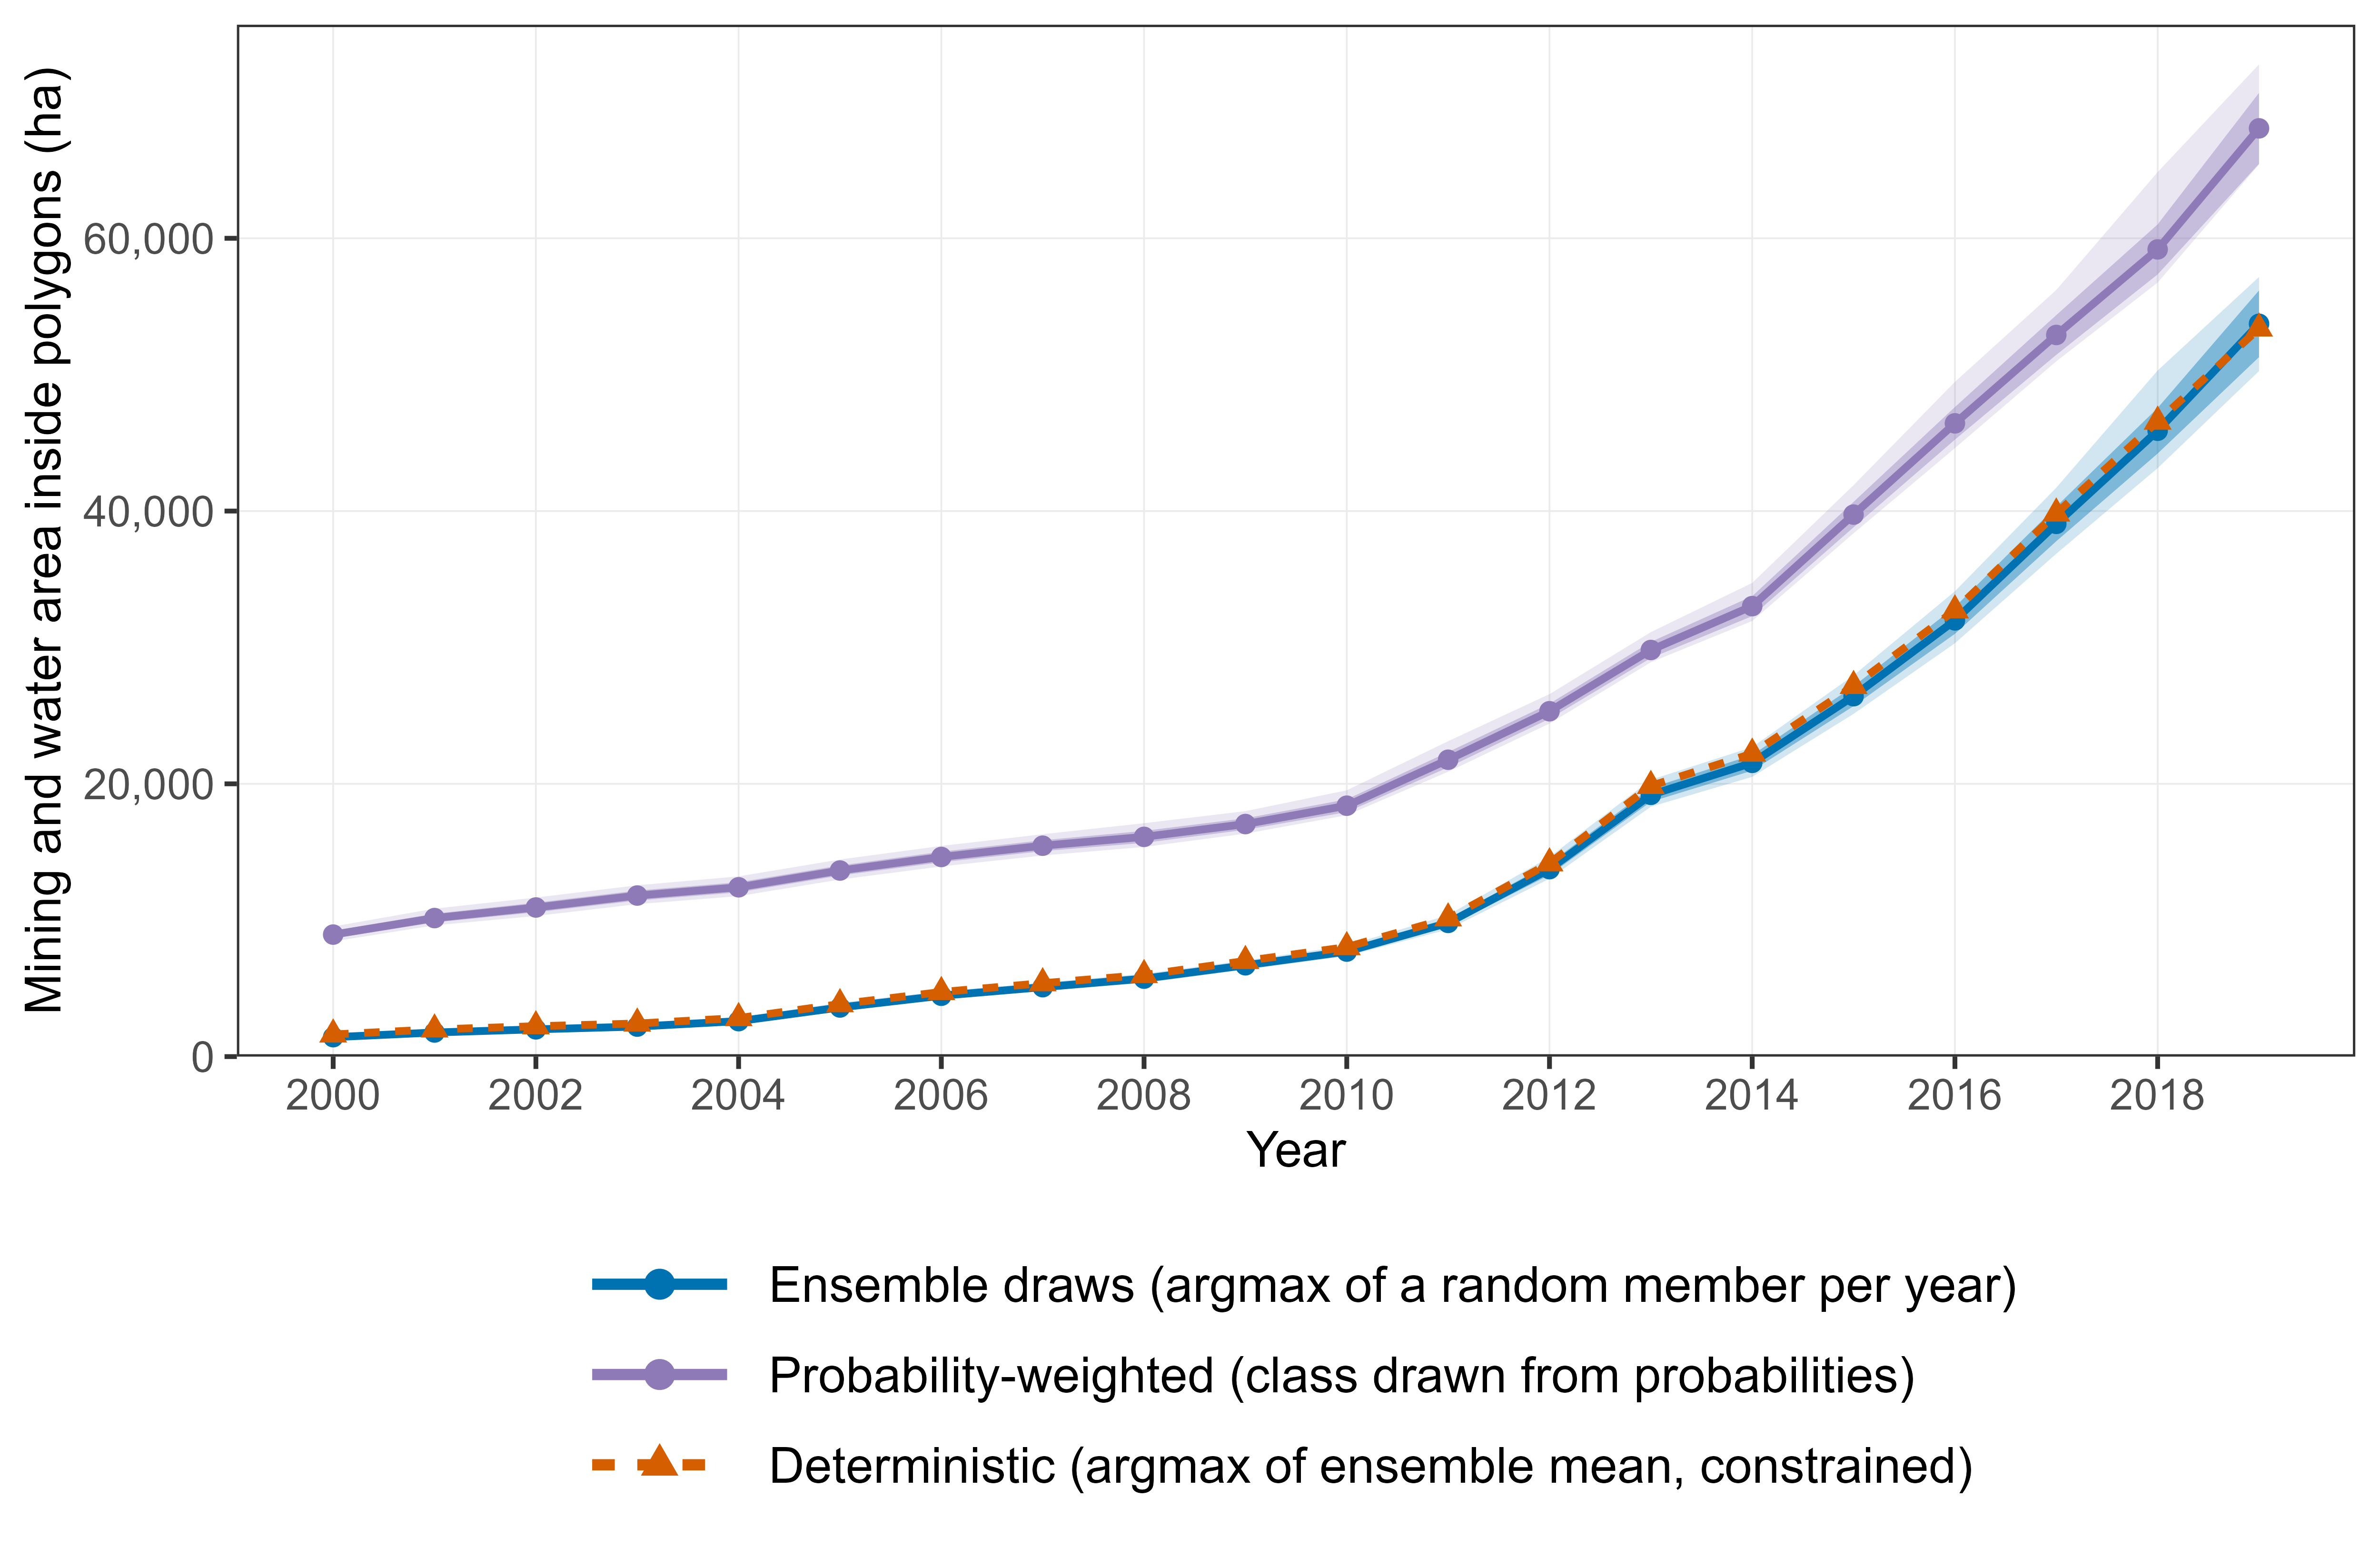
\includegraphics[width=0.85\textwidth]{figures/fig_det_vs_prob.png}
  \caption{Deterministic (argmax of the ensemble mean, then constrained)
  versus ensemble draws (argmax of a randomly drawn member per year) versus
  probability-weighted draws (class sampled from the member probabilities),
  disturbed area within polygons. Shaded bands show $\pm$1 SD (dark) and the
  95\% interval (light).}
  \label{fig:det_prob}
\end{figure}

\subsection{District mining expansion trends}
\label{app:districts}

\begin{table}[H]
\centering
\caption{Estimated mining area within polygons (mining $+$ water), \textbf{Tarkwa Nsuaem} (the merged Tarkwa Nsuaem, Prestea and Huni Valley districts), 2000 to 2019. The constrained estimate applies the transition rule. $z$-scores are computed against the district mean annual change ($\bar{x} = 388$~ha, $s = 191$~ha). Years with $z > 1.5$ in \textbf{bold}.}
\label{tab:district_tarkwa}
\small
\begin{tabular}{@{}rrrrr@{}}
\toprule
Year & \makecell[r]{Unconstr.\\(ha)} & \makecell[r]{Constr.\\(ha)} & \makecell[r]{Annual\\change (ha)} & $z$-score \\
\midrule
      2000 & 4\,239 & 783 & --- & --- \\
      2001 & 3\,750 & 1\,012 & 230 & $-$0.83 \\
      2002 & 3\,990 & 1\,169 & 157 & $-$1.20 \\
      2003 & 4\,769 & 1\,291 & 122 & $-$1.39 \\
      2004 & 6\,522 & 1\,555 & 263 & $-$0.65 \\
      2005 & 6\,563 & 1\,988 & 433 & \phantom{$-$}0.24 \\
      2006 & 6\,198 & 2\,298 & 310 & $-$0.40 \\
      2007 & 6\,698 & 2\,503 & 204 & $-$0.96 \\
      2008 & 6\,751 & 2\,695 & 192 & $-$1.02 \\
      2009 & 7\,382 & 3\,086 & 391 & \phantom{$-$}0.02 \\
      2010 & 7\,253 & 3\,364 & 278 & $-$0.57 \\
      2011 & 8\,901 & 3\,865 & 502 & \phantom{$-$}0.60 \\
      2012 & 8\,388 & 4\,409 & 544 & \phantom{$-$}0.82 \\
      2013 & 7\,178 & 4\,844 & 435 & \phantom{$-$}0.25 \\
      2014 & 6\,977 & 5\,110 & 266 & $-$0.64 \\
      2015 & 7\,266 & 5\,509 & 399 & \phantom{$-$}0.06 \\
      2016 & 7\,664 & 5\,972 & 463 & \phantom{$-$}0.39 \\
      \textbf{2017} & \textbf{8\,203} & \textbf{6\,708} & \textbf{736} & \textbf{\phantom{$-$}1.82} \\
      \textbf{2018} & \textbf{8\,150} & \textbf{7\,426} & \textbf{718} & \textbf{\phantom{$-$}1.73} \\
      \textbf{2019} & \textbf{8\,149} & \textbf{8\,149} & \textbf{723} & \textbf{\phantom{$-$}1.75} \\
\bottomrule
\end{tabular}
\end{table}

\begin{table}[H]
\centering
\caption{Estimated mining area within polygons (mining $+$ water), \textbf{Amansie West} (Amansie West district), 2000 to 2019. The constrained estimate applies the transition rule. $z$-scores are computed against the district mean annual change ($\bar{x} = 580$~ha, $s = 678$~ha). Years with $z > 1.5$ in \textbf{bold}.}
\label{tab:district_amansie}
\small
\begin{tabular}{@{}rrrrr@{}}
\toprule
Year & \makecell[r]{Unconstr.\\(ha)} & \makecell[r]{Constr.\\(ha)} & \makecell[r]{Annual\\change (ha)} & $z$-score \\
\midrule
      2000 & 3\,877 & 150 & --- & --- \\
      2001 & 2\,194 & 183 & 32 & $-$0.81 \\
      2002 & 2\,271 & 199 & 17 & $-$0.83 \\
      2003 & 3\,803 & 211 & 11 & $-$0.84 \\
      2004 & 4\,955 & 221 & 11 & $-$0.84 \\
      2005 & 3\,162 & 244 & 23 & $-$0.82 \\
      2006 & 1\,474 & 284 & 40 & $-$0.80 \\
      2007 & 1\,676 & 302 & 18 & $-$0.83 \\
      2008 & 1\,842 & 338 & 35 & $-$0.80 \\
      2009 & 2\,911 & 460 & 122 & $-$0.68 \\
      2010 & 1\,463 & 607 & 148 & $-$0.64 \\
      2011 & 2\,228 & 862 & 255 & $-$0.48 \\
      2012 & 4\,096 & 1\,820 & 958 & \phantom{$-$}0.56 \\
      \textbf{2013} & \textbf{6\,331} & \textbf{3\,854} & \textbf{2\,033} & \textbf{\phantom{$-$}2.14} \\
      2014 & 6\,797 & 4\,487 & 633 & \phantom{$-$}0.08 \\
      2015 & 8\,502 & 6\,044 & 1\,557 & \phantom{$-$}1.44 \\
      2016 & 10\,189 & 7\,468 & 1\,425 & \phantom{$-$}1.24 \\
      2017 & 11\,182 & 8\,935 & 1\,466 & \phantom{$-$}1.31 \\
      2018 & 10\,943 & 10\,003 & 1\,068 & \phantom{$-$}0.72 \\
      2019 & 11\,178 & 11\,178 & 1\,176 & \phantom{$-$}0.88 \\
\bottomrule
\end{tabular}
\end{table}

\begin{table}[H]
\centering
\caption{Estimated mining area within polygons (mining $+$ water), \textbf{Wassa Amenfi} (the merged Wassa Amenfi East and West districts), 2000 to 2019. The constrained estimate applies the transition rule. $z$-scores are computed against the district mean annual change ($\bar{x} = 610$~ha, $s = 896$~ha). Years with $z > 1.5$ in \textbf{bold}.}
\label{tab:district_wassa}
\small
\begin{tabular}{@{}rrrrr@{}}
\toprule
Year & \makecell[r]{Unconstr.\\(ha)} & \makecell[r]{Constr.\\(ha)} & \makecell[r]{Annual\\change (ha)} & $z$-score \\
\midrule
      2000 & 3\,156 & 76 & --- & --- \\
      2001 & 1\,397 & 82 & 7 & $-$0.67 \\
      2002 & 1\,950 & 86 & 3 & $-$0.68 \\
      2003 & 5\,518 & 94 & 8 & $-$0.67 \\
      2004 & 6\,827 & 101 & 6 & $-$0.67 \\
      2005 & 5\,730 & 114 & 14 & $-$0.67 \\
      2006 & 3\,345 & 134 & 20 & $-$0.66 \\
      2007 & 3\,972 & 158 & 23 & $-$0.65 \\
      2008 & 2\,910 & 196 & 38 & $-$0.64 \\
      2009 & 3\,140 & 304 & 108 & $-$0.56 \\
      2010 & 2\,796 & 408 & 104 & $-$0.57 \\
      2011 & 4\,930 & 599 & 191 & $-$0.47 \\
      2012 & 4\,305 & 1\,000 & 402 & $-$0.23 \\
      2013 & 3\,190 & 1\,509 & 508 & $-$0.11 \\
      2014 & 3\,558 & 1\,920 & 411 & $-$0.22 \\
      2015 & 5\,066 & 2\,930 & 1\,010 & \phantom{$-$}0.45 \\
      2016 & 7\,663 & 4\,408 & 1\,477 & \phantom{$-$}0.97 \\
      \textbf{2017} & \textbf{10\,563} & \textbf{6\,785} & \textbf{2\,377} & \textbf{\phantom{$-$}1.97} \\
      \textbf{2018} & \textbf{11\,770} & \textbf{9\,467} & \textbf{2\,682} & \textbf{\phantom{$-$}2.31} \\
      \textbf{2019} & \textbf{11\,657} & \textbf{11\,657} & \textbf{2\,190} & \textbf{\phantom{$-$}1.76} \\
\bottomrule
\end{tabular}
\end{table}
 
\begin{table}[H]
\centering
\caption{Estimated mining area within polygons (mining $+$ water), \textbf{Upper Denkyira} (the merged Upper Denkyira East and West districts), 2000 to 2019. The constrained estimate applies the transition rule. $z$-scores are computed against the district mean annual change ($\bar{x} = 330$~ha, $s = 346$~ha). Years with $z > 1.5$ in \textbf{bold}.}
\label{tab:district_denkyira}
\small
\begin{tabular}{@{}rrrrr@{}}
\toprule
Year & \makecell[r]{Unconstr.\\(ha)} & \makecell[r]{Constr.\\(ha)} & \makecell[r]{Annual\\change (ha)} & $z$-score \\
\midrule
      2000 & 1\,251 & 68 & --- & --- \\
      2001 & 780 & 78 & 10 & $-$0.93 \\
      2002 & 1\,045 & 81 & 3 & $-$0.94 \\
      2003 & 2\,276 & 86 & 5 & $-$0.94 \\
      2004 & 2\,466 & 87 & 1 & $-$0.95 \\
      2005 & 1\,506 & 99 & 13 & $-$0.92 \\
      2006 & 696 & 121 & 22 & $-$0.89 \\
      2007 & 1\,116 & 136 & 14 & $-$0.91 \\
      2008 & 1\,107 & 160 & 24 & $-$0.88 \\
      2009 & 1\,786 & 270 & 110 & $-$0.64 \\
      2010 & 1\,224 & 464 & 194 & $-$0.39 \\
      2011 & 2\,377 & 918 & 454 & \phantom{$-$}0.36 \\
      2012 & 3\,201 & 1\,700 & 781 & \phantom{$-$}1.30 \\
      \textbf{2013} & \textbf{3\,803} & \textbf{2\,669} & \textbf{969} & \textbf{\phantom{$-$}1.85} \\
      2014 & 3\,961 & 2\,934 & 265 & $-$0.19 \\
      2015 & 4\,721 & 3\,556 & 622 & \phantom{$-$}0.84 \\
      2016 & 5\,725 & 4\,277 & 721 & \phantom{$-$}1.13 \\
      2017 & 6\,422 & 5\,078 & 801 & \phantom{$-$}1.36 \\
      2018 & 6\,392 & 5\,752 & 673 & \phantom{$-$}0.99 \\
      2019 & 6\,343 & 6\,343 & 591 & \phantom{$-$}0.75 \\
\bottomrule
\end{tabular}
\end{table}
 
\begin{table}[H]
\centering
\caption{Estimated mining area within polygons (mining $+$ water), \textbf{Asutifi} (Asutifi district), 2000 to 2019. The constrained estimate applies the transition rule. $z$-scores are computed against the district mean annual change ($\bar{x} = 107$~ha, $s = 102$~ha). Years with $z > 1.5$ in \textbf{bold}.}
\label{tab:district_asutifi}
\small
\begin{tabular}{@{}rrrrr@{}}
\toprule
Year & \makecell[r]{Unconstr.\\(ha)} & \makecell[r]{Constr.\\(ha)} & \makecell[r]{Annual\\change (ha)} & $z$-score \\
\midrule
      2000 & 700 & 1 & --- & --- \\
      2001 & 141 & 1 & 0 & $-$1.05 \\
      2002 & 8 & 2 & 1 & $-$1.04 \\
      2003 & 11 & 3 & 1 & $-$1.04 \\
      2004 & 28 & 13 & 11 & $-$0.95 \\
      \textbf{2005} & \textbf{693} & \textbf{381} & \textbf{368} & \textbf{\phantom{$-$}2.55} \\
      \textbf{2006} & \textbf{985} & \textbf{660} & \textbf{279} & \textbf{\phantom{$-$}1.68} \\
      2007 & 1\,274 & 912 & 252 & \phantom{$-$}1.42 \\
      2008 & 1\,575 & 1\,114 & 203 & \phantom{$-$}0.93 \\
      2009 & 1\,580 & 1\,210 & 96 & $-$0.11 \\
      2010 & 1\,596 & 1\,304 & 94 & $-$0.13 \\
      2011 & 1\,754 & 1\,444 & 140 & \phantom{$-$}0.32 \\
      2012 & 1\,881 & 1\,543 & 99 & $-$0.08 \\
      2013 & 1\,996 & 1\,659 & 116 & \phantom{$-$}0.09 \\
      2014 & 2\,145 & 1\,771 & 112 & \phantom{$-$}0.04 \\
      2015 & 2\,107 & 1\,800 & 29 & $-$0.77 \\
      2016 & 2\,141 & 1\,860 & 60 & $-$0.46 \\
      2017 & 2\,134 & 1\,918 & 58 & $-$0.48 \\
      2018 & 2\,123 & 1\,968 & 50 & $-$0.56 \\
      2019 & 2\,039 & 2\,039 & 71 & $-$0.35 \\
\bottomrule
\end{tabular}
\end{table}

\section{Variable selection and model comparison}
\label{app:benchmarks}
Recently, attention has been pointed towards local ecological realities and implications for effective land cover classification across heterogenous landscapes \citep{zhang2026Geographical,phiri2017Developments,shen2022bidirectional}. Therefore, I investigated how my national model performs against ecological zone specific models, in different areas of Ghana, and how zone-specific features as informed by literature perform against data-driven feature selection \citep{chen2025Spectral} (See appendix section C). In my study, where I modelled Ghana's three ecological zones after \citet{yamba2023Revisiting}, I find that zone-specific models were statistically indistinguishable from a national model. However, the comparison revealed some meaningful nuances. Whilst a national model handles local signature differences implicitly (Larger feature set and sample size), different features impacted mining F1 in different parts of Ghana. For example, whilst the Forest-Transition zone showed good detection accuracy across classes (Mining F1 = 0.82; Water F1 = 0.92; Vegetation F1 = 0.89), the Northern zone showed more variability with a lower mining F1 of 0.56 and perfect water detection of F1 = 1.0. The feature importance test reveals that bare soil signatures play an important role, with BSI, CLAY and SWIR features dominating mining detection in the coastal zone, whilst BSI and NDBI, as well as NIR texture are important features for detection in the North. Overall, vegetation and mining were most often confused by the model, indicating the class confusion in the less-vegetated North, as well as confusion between shrubland and small mines in other zones.

Generally, this indicates that literature informed ecological zones matter and that a combination of data- and literature-informed, zone-specific variables (E.g. emphasising NDVI, SWIR, and texture metrics) can capture real ecological differences associated with local mining characteristics. The fact, that zone-specific feature sets, and zone-specific models performed as well as a national model calls for the importance of these features and classification areas grounded in ecology, as they are more interpretable. 

A conducted power analysis \citep{buda2018systematic} indicates that the national model is defensible for my use case but observed zone-specific performances suggest attention must be placed on ecological realities. Therein, my approach suggests that future work must take into account the unique spectral variations found across diverse ecological landscapes. Using verified feature sets for different ecological zones can help us improve classification accuracy and interpretability.

The mediocre performance of my northern zone on the other hand is rooted in the fact that only one small mining site (near Tinga in Savannah region) of the \citet{maus2020globalscale} polygons falls into these latitudes, resulting in few, clustered mining samples. If future studies seek to focus on mining detection in Ghana's north, I suggest training separate models for this zone and type of vegetation.

\subsection{Feature selection}
\label{app:features}
The 2010 composite (example) was created from five to ten valid dry season pictures across 2009, 2010, and 2011, leaving the best medoid scene-images for the final composite creation. This approach follows recommendations by \citet{flood2013Seasonal} who demonstrated that medoid-based selection preserves spectral relationships between bands better than simple median or maximum NDVI compositing. I excluded scenes that showed more than 50\% cloud cover.

Landsat 5 TM and Landsat 7 ETM+ were used for composites from 2000 through 2012, transitioning to Landsat 7, and 8 OLI for subsequent years. Cross-calibration between sensors followed \citet{roy2016Characterization} and USGS Collection 2 Level-2 surface reflectance specifications \citep{usgs2022Landsat}. I addressed Landsat 7 scan-line corrector failures by filling the gaps with overlapping observations from adjacent dates and sensors within each three-year window. Cloud masking utilized the QA\_PIXEL band\footnote{For more information on data quality and availability see Appendix D.}.

I included surface reflactance in blue, green, and red, as well as near infrared (NIR) and short-wave infrared (SWIR), which provide good information for mineral detection \citep{koerting2024VNIRSWIR}. Several spectral indices were then derived from the original bands, enabling better discrimination based on reflectance values and ecological knowledge. The Normalized Difference Vegetation Index \citep[NDVI;][]{tucker1979Red,rouse1973Monitoring} was calculated for vegetation discrimination, whilst the Bare Soil Index \citep[BSI;][]{rikimaru2002Tropical} and modified BSI \citep{nguyen2021Modified} were used for soil detection. Water indices used include NDWI, Modified NDWI \citep[MNDWI;][]{xu2006Modification}, and Automated Water Extraction Index \citep[AWEI;][]{feyisa2014Automated} for tailing pond detection, and mining along river systems. An Urban Index \citep[UI;][]{javed2021Review} was employed alongside iron oxide ratios (red/blue) and clay indices (SWIR1/SWIR2) as potential indicators of mineralization \citep{barenblitt2021large}.

Adding to these, I included topographic information such as elevation, slope, aspect, and the Terrain Ruggedness Index (TRI) derived from SRTM 30~m data \citep{farr2007Shuttle,barenblitt2021large,svoboda2022Random}. Additionally, I used grey-level co-occurrence matrix (GLCM) features such as contrast, correlation, variance, and entropy, calculated from the NIR band at 3$\times$3 pixel windows \citep{haralick1973Textural} to leverage local variance and higher contrast at mining sites (E.g. pits, stockpiles, roads) as compared to natural bare surfaces.

Lastly, I employed temporal metrics such as standard deviation of NIR, red, and SWIR1 bands across the three-year compositing window to capture intra-period variability potentially associated with active mining expansion. An NDVI anomaly layer was calculated as the difference between each year's NDVI and a baseline mean NDVI (Permutation-based from 2000 to 2004), providing a vegetation disturbance indicator relative to pre-mining conditions \citep{barenblitt2021large}. A full list of variables found in each composite, as well as their value ranges is shown below.

I also tested zone-specific features as I assumed local spectral signatures, vegetation, and mining types differ, demanding consideration of varying variables to include for model training. I balanced correlation of variables (For example water index family)\citep{hooker2021Unrestricted}, statistical significance of inclusion of a variable, and ecological knowledge from literature. I report standard permutation (Just to showcase the correlation of indices as pointed out by e.g. \citet{hooker2021Unrestricted}), clustered permutation (Leaving out entire groups of variables when they are highly correlated such as e.g. the water indices), and a `per feature, per zone, per fold' selection leaving individual variables, and their correlated `clusters' out to establish their importance for classification. The top-k features of this data-driven selection are then tested using spatial clustering against (and combining) literature-derived feature selection using the \citet{mcnemar1947Note} test to determine whether one feature-set is significantly better at discriminating land cover. The validation showed no statistically significant improvement of using zone-specific feature sets and models (As will be discussed later). Therefore, all features were used to train the national RF classifier.

\begin{table}[H]
\centering
\caption{The 27 bands of the national random forest. All bands are computed from annual Landsat medoid composites (2000 to 2019) and SRTM. Model input range: values are clipped to these limits before training and prediction. Not used: entropy (constant in the 2019 training composite), nightlight bands (sensor change from DMSP to VIIRS in 2013) and composite quality bands.}
\label{tab:variables}
\resizebox{\textwidth}{!}{%
\begin{tabular}{@{}llll@{}}
\toprule
\textbf{Category} & \textbf{Variable} & \textbf{Description} & \textbf{Model input range} \\
\midrule
\multirow{6}{*}{Spectral}
& BLUE  & Blue surface reflectance          & [0.000, 0.250] \\
& GREEN & Green surface reflectance         & [0.000, 0.250] \\
& RED   & Red surface reflectance           & [0.000, 0.350] \\
& NIR   & Near-infrared surface reflectance & [0.000, 0.750] \\
& SWIR1 & Short-wave infrared 1 reflectance & [0.000, 0.750] \\
& SWIR2 & Short-wave infrared 2 reflectance & [0.000, 0.700] \\
\midrule
\multirow{12}{*}{Spectral indices}
& NDVI        & Normalised difference vegetation index          & [$-$1.000, 1.000] \\
& NDWI        & Normalised difference water index (green, NIR)  & [$-$1.000, 1.000] \\
& MNDWI       & Modified NDWI (green, SWIR1)                    & [$-$1.000, 1.000] \\
& AWEI\_NSH   & Automated water extraction index, no shadow     & [$-$10.0, 5.000] \\
& AWEI\_SH    & Automated water extraction index, shadow        & [$-$10.0, 5.000] \\
& BSI         & Bare soil index                                 & [$-$1.000, 1.000] \\
& NDBI        & Normalised difference built-up index            & [$-$1.000, 1.000] \\
& IRON\_OXIDE & Iron oxide ratio (red / blue)                   & [0.000, 3.000] \\
& CLAY\_INDEX & Clay mineral index (SWIR1, SWIR2)               & [$-$1.000, 1.000] \\
& CI          & Colouration index (red, green)                  & [$-$1.000, 1.000] \\
& BI          & Brightness index (visible bands)                & [0.000, 1.000] \\
& WATER\_PROB & Water probability score                         & [0.000, 3.000] \\
\midrule
\multirow{4}{*}{Texture}
& NIR\_STD\_DEV  & Local standard deviation of NIR & [0.000, 0.250] \\
& NIR\_contrast  & GLCM contrast of NIR            & unclipped \\
& NIR\_corr      & GLCM correlation of NIR         & unclipped \\
& NIR\_var       & GLCM variance of NIR            & unclipped \\
\midrule
\multirow{4}{*}{Topographic}
& ELEVATION & Elevation, SRTM (m)       & [$-$32, 850] \\
& SLOPE     & Terrain slope (degrees)   & [0.0, 75.0] \\
& ASPECT    & Terrain aspect (degrees)  & [0, 360] \\
& TRI       & Terrain ruggedness index  & [0.0, 85.0] \\
\midrule
Temporal
& NDVI\_ANOMALY & NDVI deviation from 2000--2004 baseline & [$-$1.500, 1.500] \\
\bottomrule
\end{tabular}%
}
\end{table}

A permutation analysis of related features (See below) showed that the national model's skill is spread across correlated band groups. Dropping any single feature ``family'' changed spatial-CV accuracy by at most 0.6 percentage points and mining $F_1$ by at most 1 point, well within the fold-to-fold variation (SD = 3 points). Band selection did not help either. A selection of my top 10 bands (0.858) and the 19 literature-based bands (0.859) both performed below the full 27-band model (0.870; McNemar $p = 0.034$ against the top-10 set). The literature-based and data-driven rankings overlapped only partly (Jaccard 0.32--0.50). Within the ecological zones, bare-soil indices (BSI, Clay Index) were the most influential feature group for mining $F_1$ in the coastal zone, and topography mattered in the forest-transition zone (log-loss $+0.07$ when removed). In the Northern Savannah zone, with only 46 mining samples around one site (6 to 16 per fold), feature ``family'' effects on mining $F_1$ ($\pm$4 points) were indistinguishable from fold noise (SD 13--18 points) and only the spectral water/vegetation family affected accuracy (log-loss $0.22 \rightarrow 0.34$). The zone-specific model did classify the north more accurately (0.909 vs.\ 0.859; McNemar $p = 0.005$), but equally well with literature or all 27 bands, and without improving the mining $F_1$ (+0.02, 95\% CI $-0.13$ to $+0.16$). I therefore use one national model with all bands and treat northern mining estimates as the least certain. 

Figure~\ref{fig:drop_cluster} shows drop-family importance: each correlated
group of bands (e.g.\ the water indices) is removed in turn and the model is
re-trained under spatial cross-validation. Figure~\ref{fig:feature_overlap}
compares literature-based and data-driven band sets per zone.
Figure~\ref{fig:feature_set_comparison} shows mean accuracy across the five
spatial folds with 95\% confidence intervals. All 27 candidate bands
performed best and were used for the final model.

\begin{figure}[H]
  \centering
  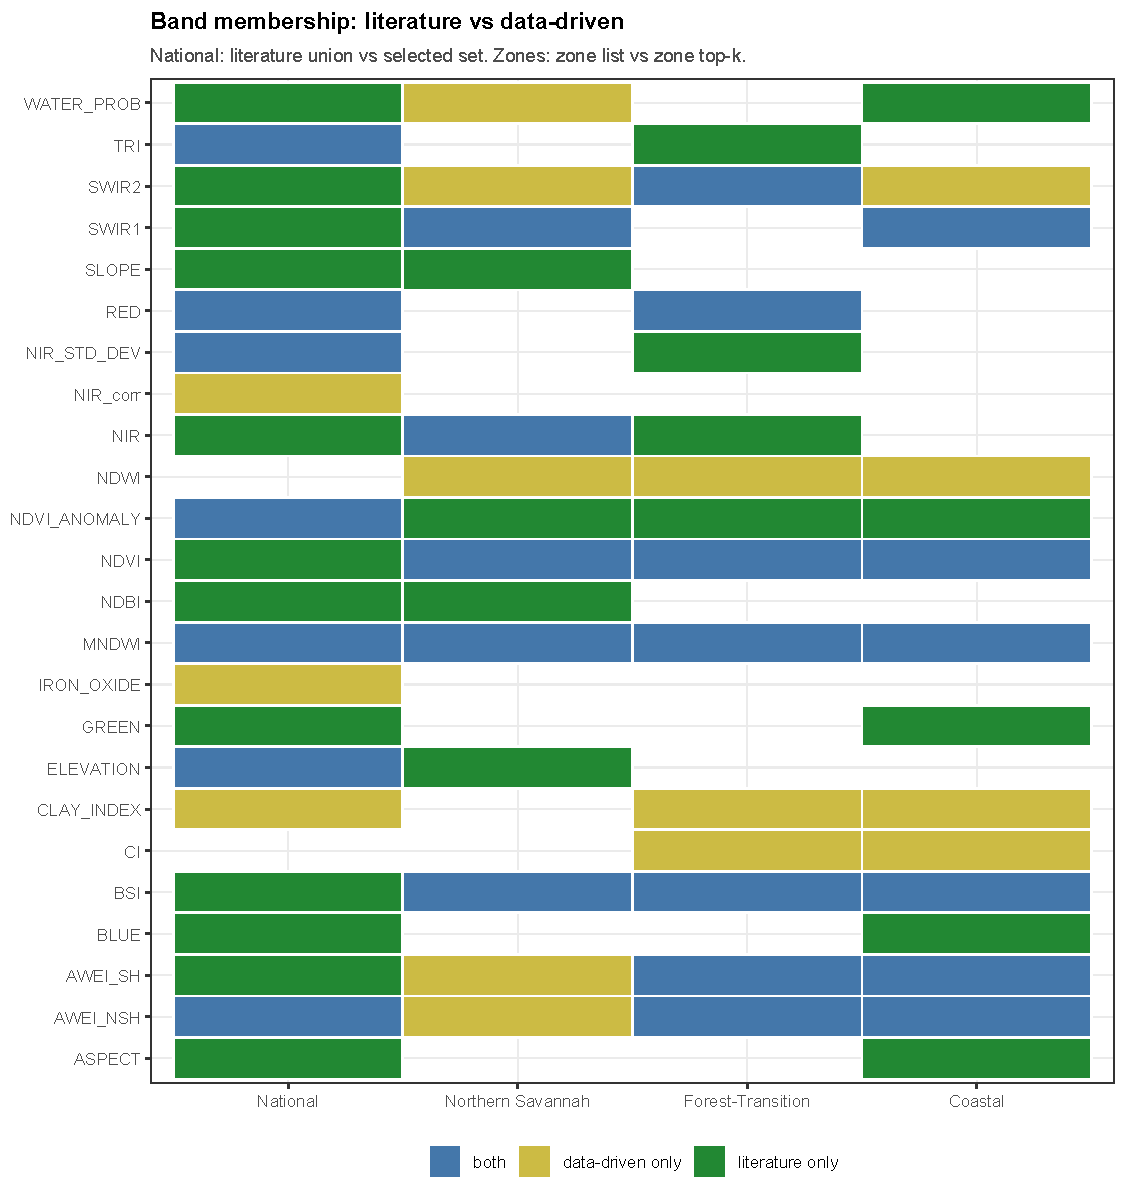
\includegraphics[width=0.85\textwidth]{figures/feature_overlap_heatmap.pdf}
  \caption{Band membership of literature-based and data-driven feature sets,
  nationally and per latitude zone.}
  \label{fig:feature_overlap}
\end{figure}

\begin{figure}[H]
  \centering
  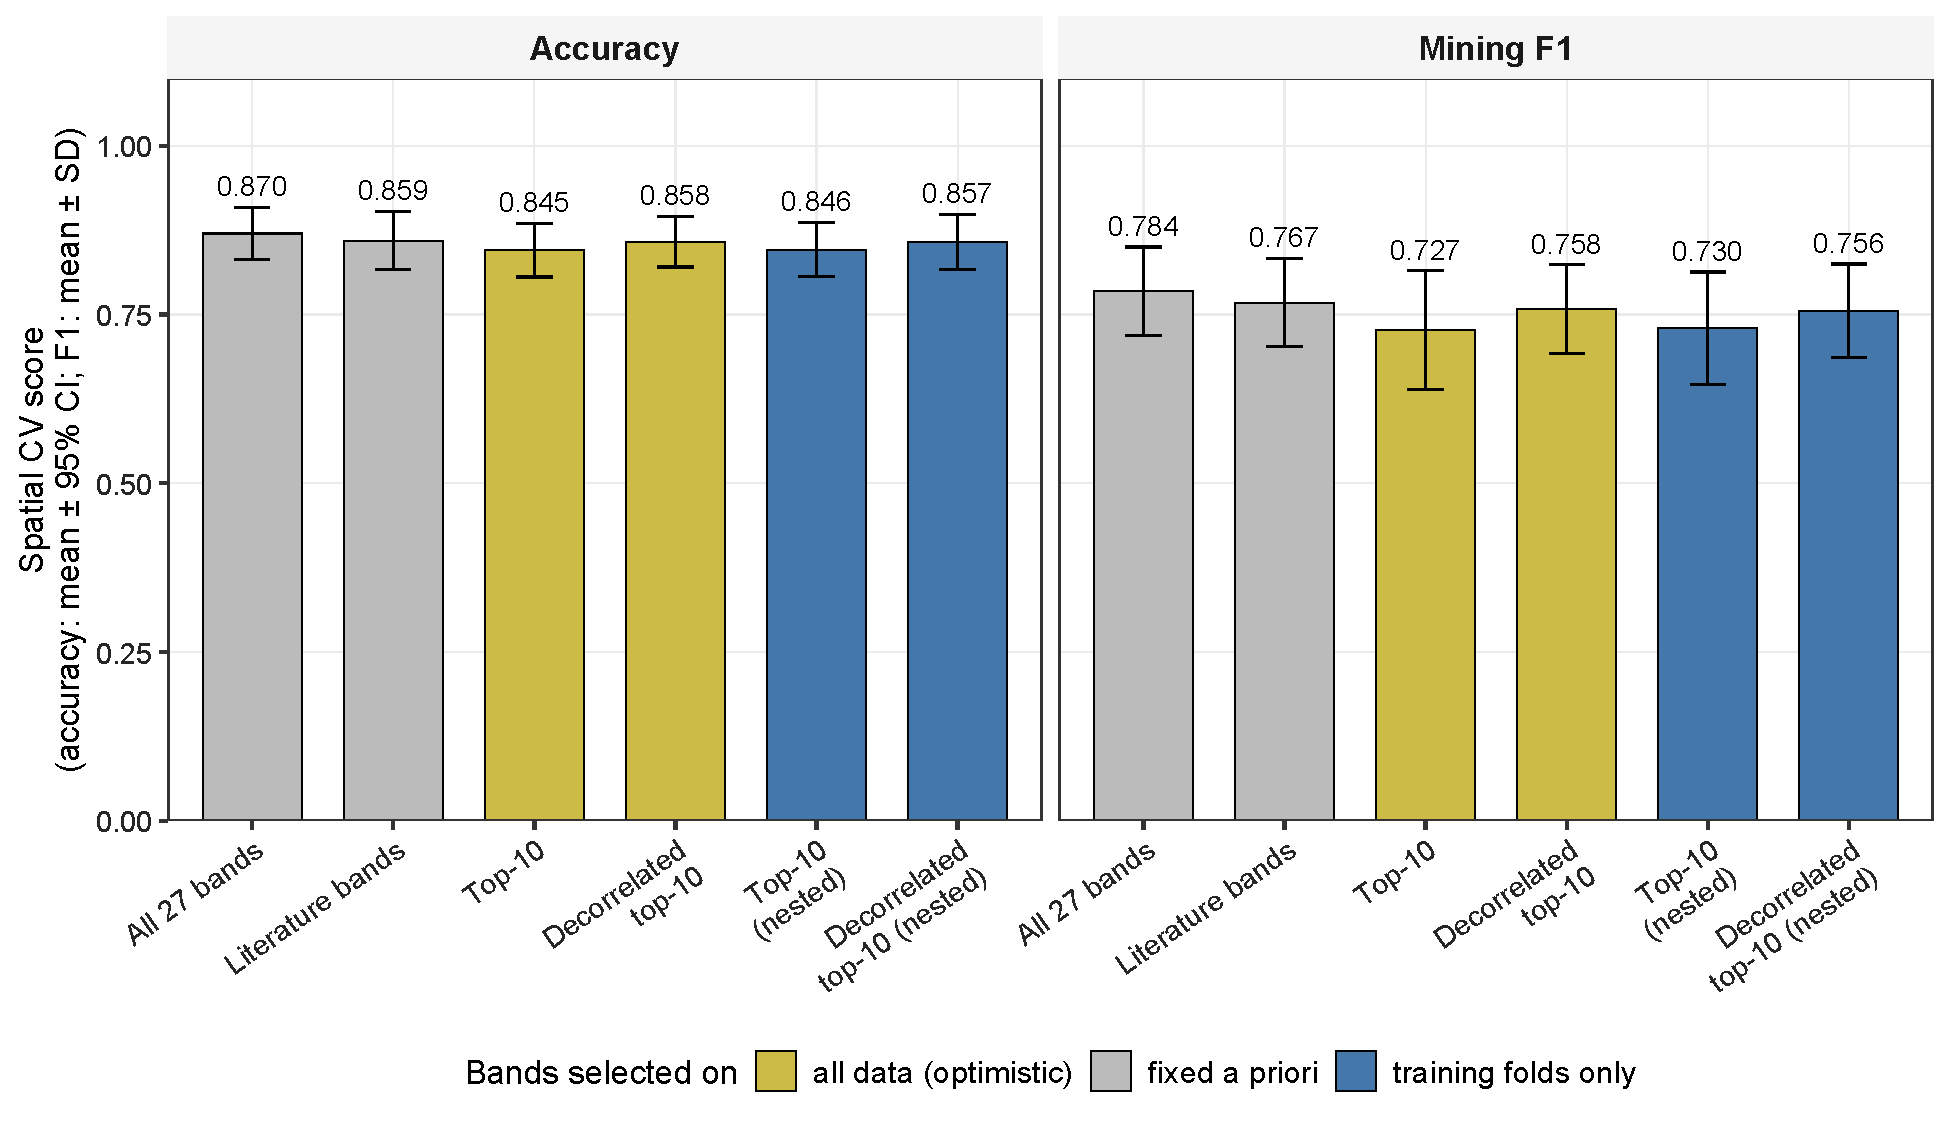
\includegraphics[width=1\textwidth]{figures/feature_set_comparison.pdf}
  \caption{National band sets under spatial cross-validation (shared folds).}
  \label{fig:feature_set_comparison}
\end{figure}

\begin{figure}[H]
  \centering
  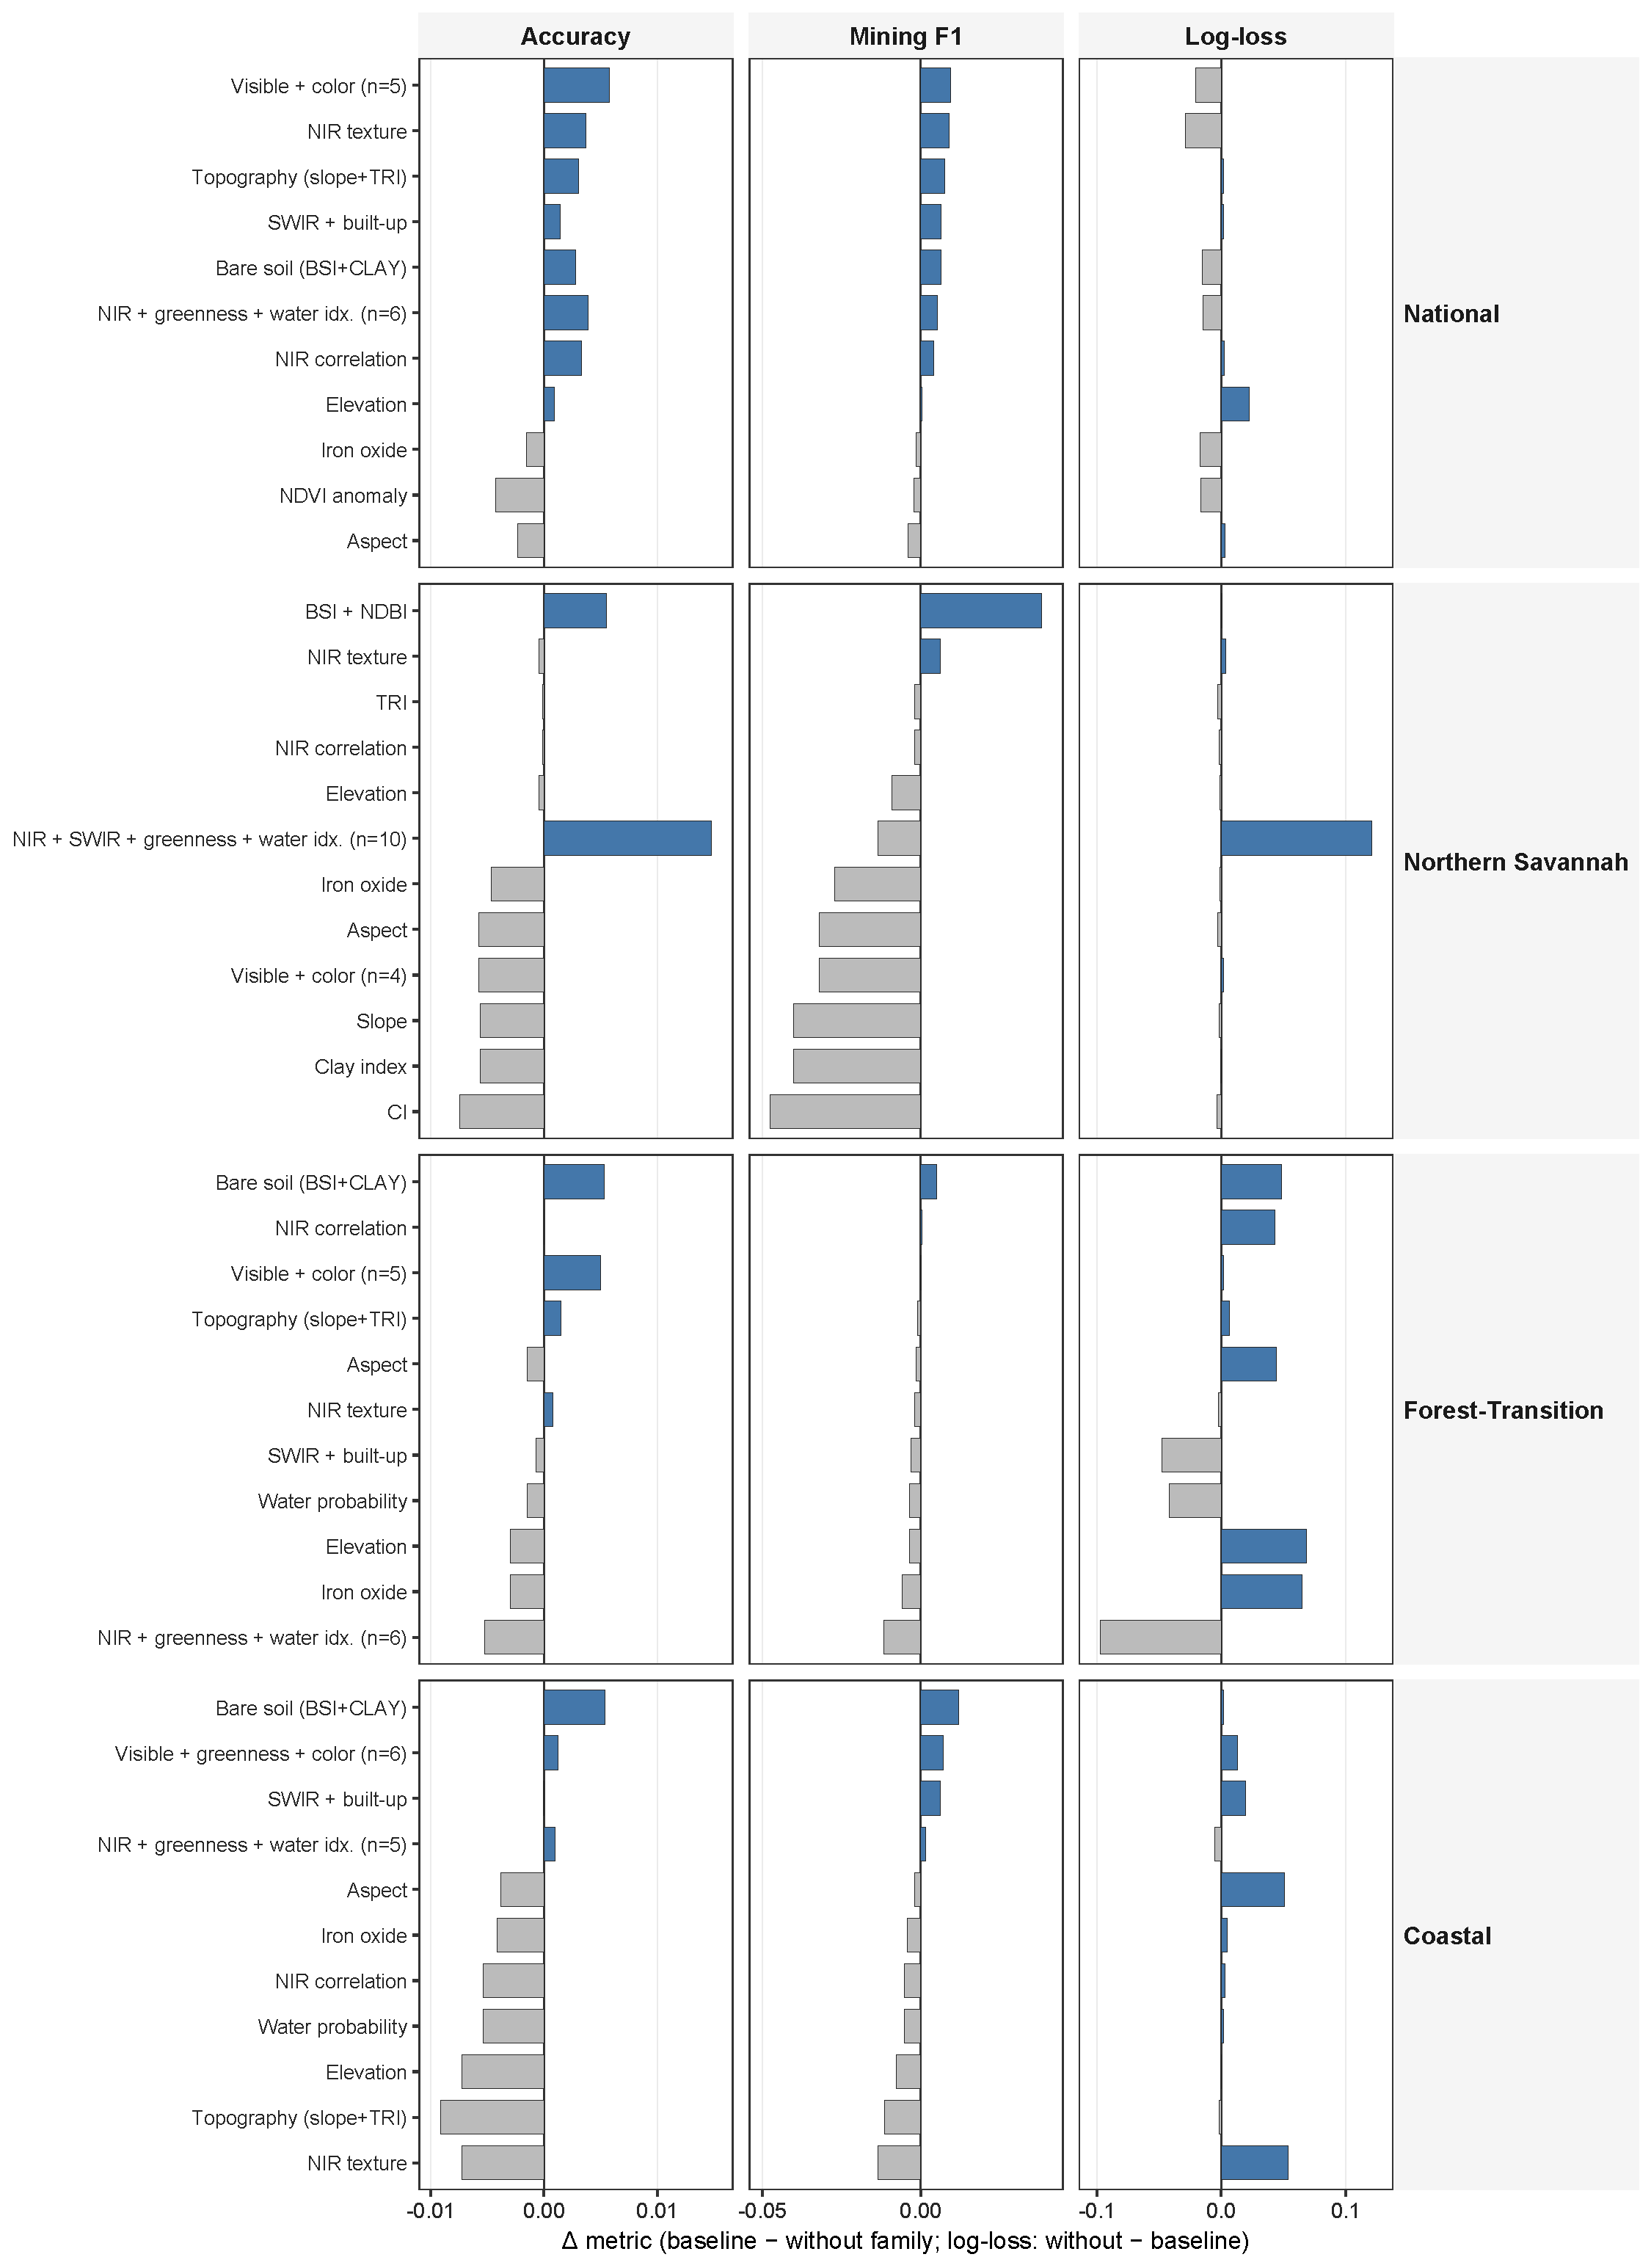
\includegraphics[width=1\textwidth]{figures/drop_cluster_importance_multimetric.pdf}
  \caption{Effect of removing each band family on mining $F_1$, accuracy and
  log-loss.}
  \label{fig:drop_cluster}
\end{figure}

\subsection{Model performance under spatial cross-validation}
Standard k-fold cross-validation overestimates accuracy by up to 50\% when training and validation samples are spatially proximate \citep{roberts2017Crossvalidation,valavi2019Block}. Since my data is naturally clustered around mining sites and along river systems, I implemented spatial blocking cross-validation with five folds, using the \texttt{blockCV} package \citep{valavi2019Block} to divide my training and test data into spatially separate blocks within each fold \citep{meyer2018Improving}. Training samples falling within the buffer around test blocks were excluded from that fold's training set. This approach provides more conservative and realistic accuracy estimates compared to random cross-validation \citep{ploton2020Spatial,valavi2019Block}. Based on my training data location I then conducted an `area of applicability' analysis as advocated for by \citet{meyer2021Predicting} to assess the distance between points necessary to achieve `spatial independence' and to compute block sizes appropriate for my data. These variograms assess the change in similarity between observations as distance between them is increased, resulting in a range needed to find data points that are uncorrelated.  

As visible below in Figure \ref{fig:fig_methods_panel}, these variograms computed buffer sizes of 2,2~km. This range is used as buffer distance in the 5-fold cross-validation.

\begin{figure}[H]
    \centering
    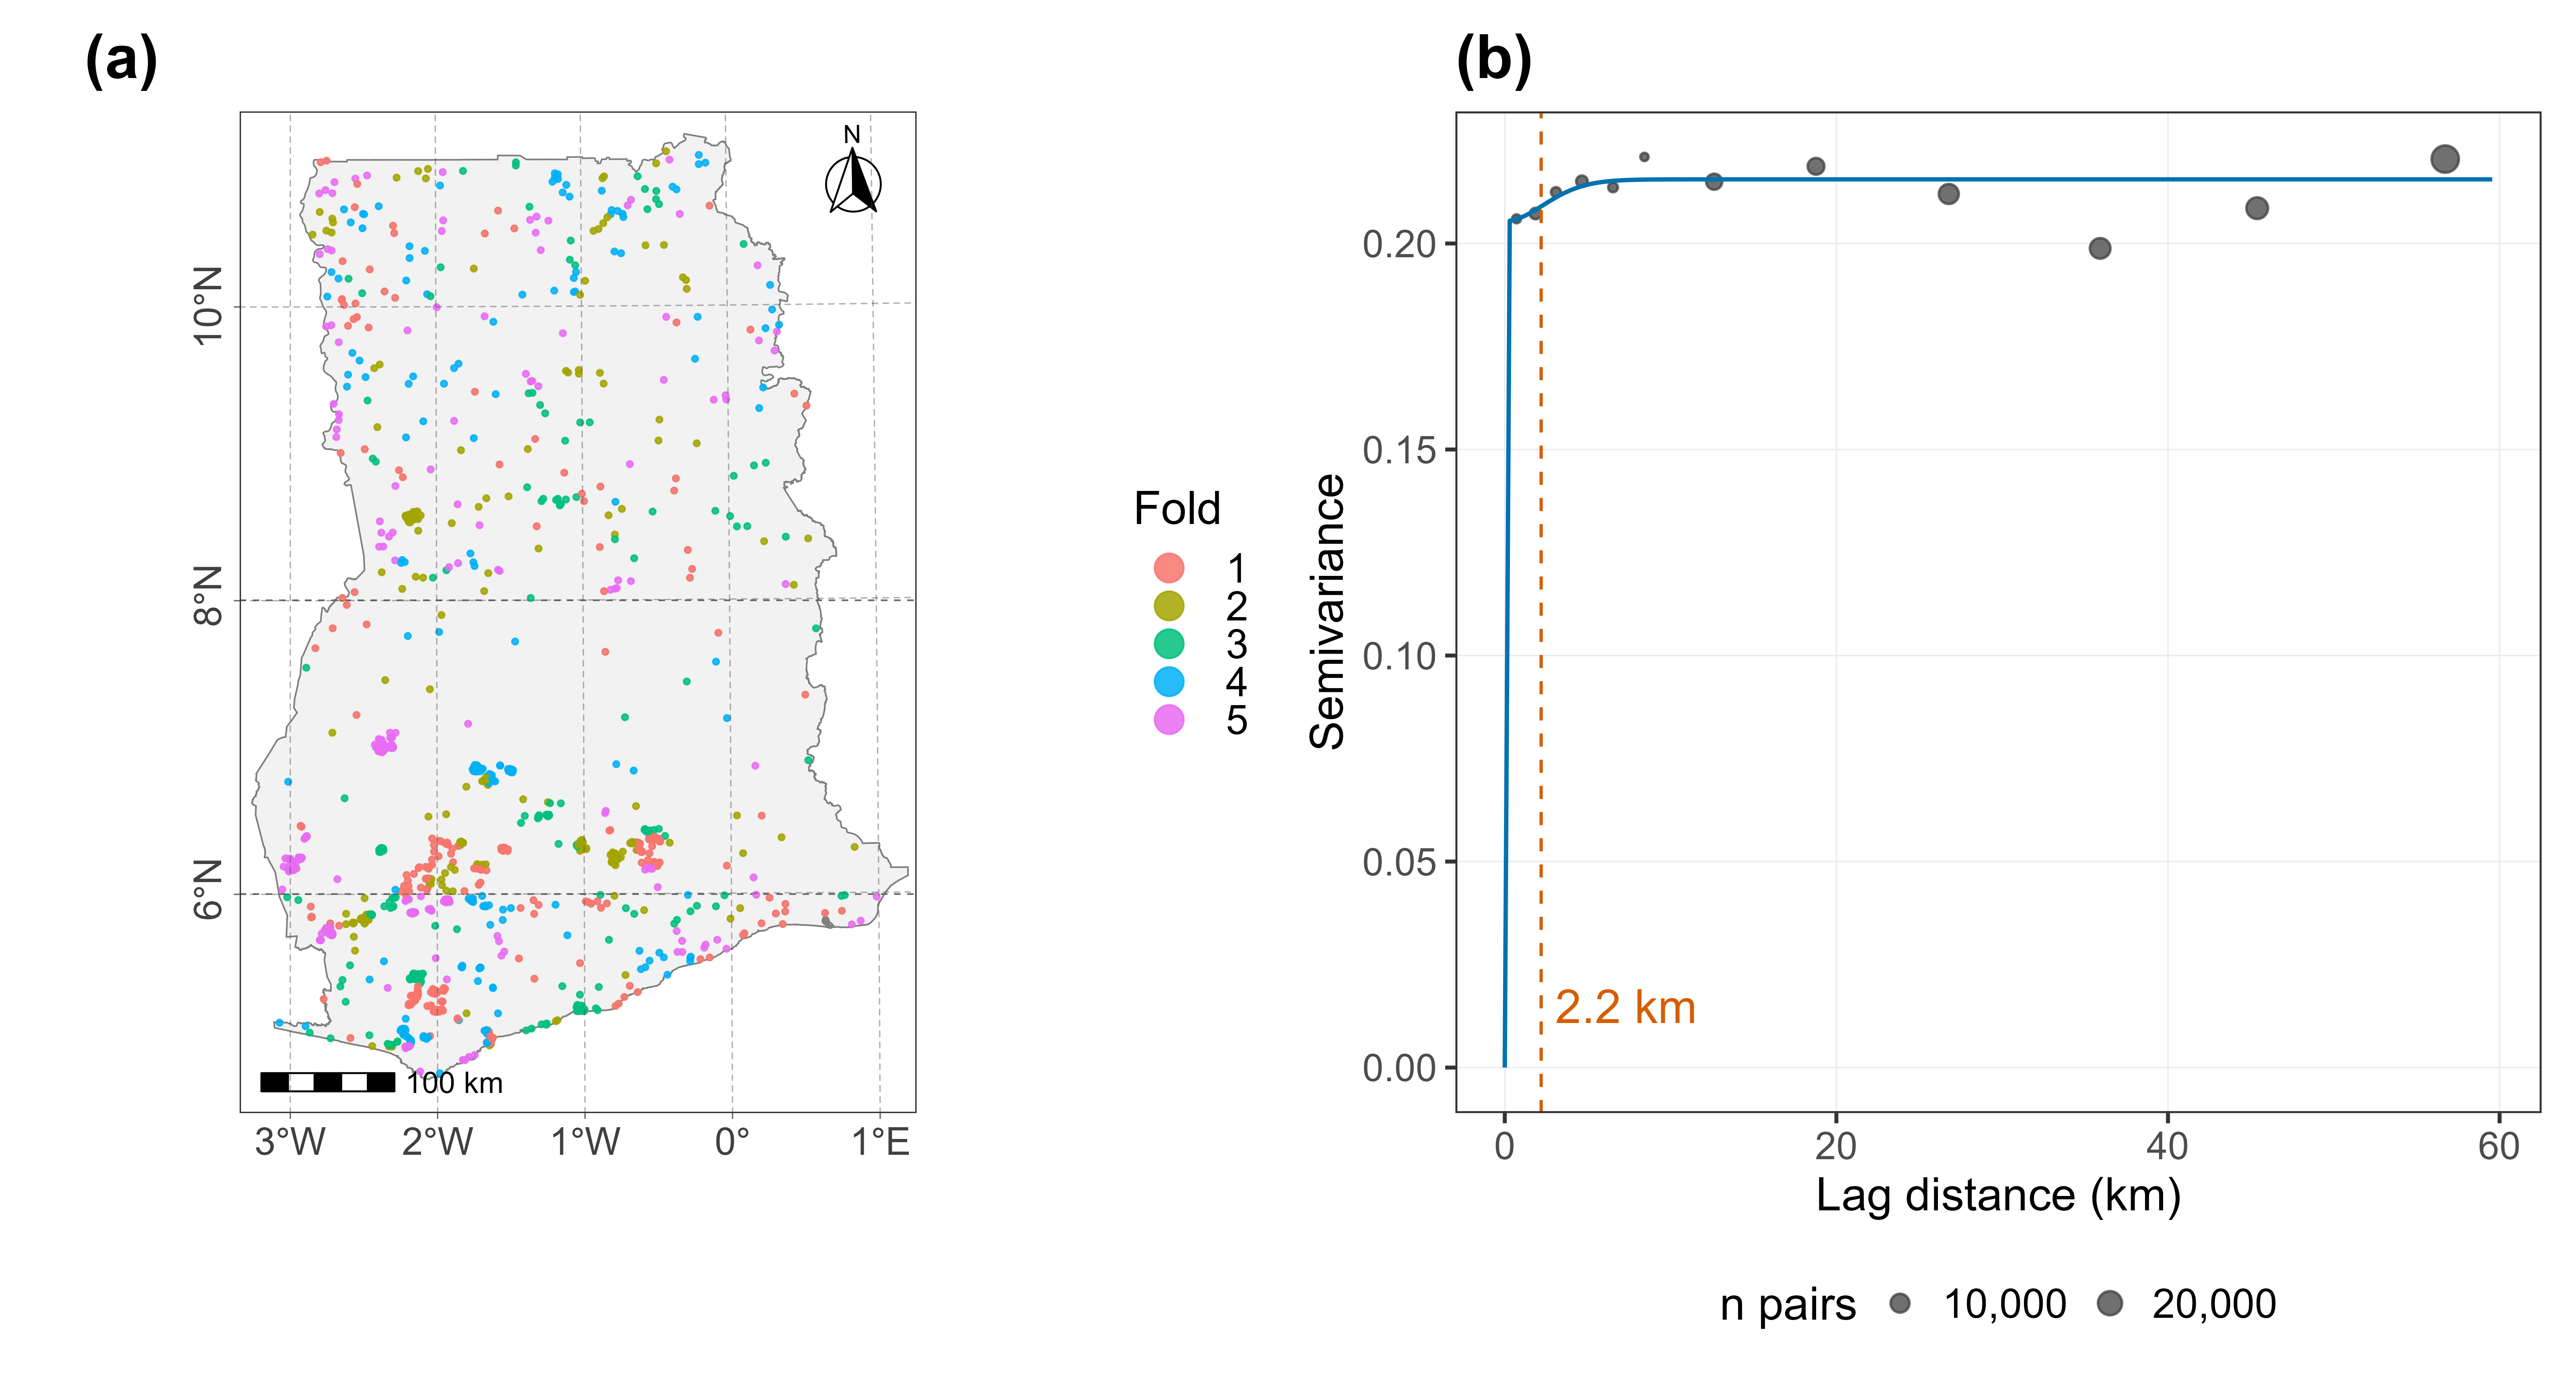
\includegraphics[width=0.9\textwidth]{figures/fig_methods_panel.png}
    \caption{Spatial blocks (a) and Variogram fits (b) for spatial CV.}
    \label{fig:fig_methods_panel}
\end{figure}

\label{app:performance}
To evaluate whether ecological zoning and zone-specific feature selection provide measurable improvements over national or uniform feature approaches, I conducted a systematic comparison using the the same spatial folds and 22.5~km blocks\footnote{Compromise between the different zone-specific buffer distances for comparability.} across the following configurations (See table~\ref{tab:benchmark_master} below). Three alternative combinations beside my national model (P0 - single national random forest model trained on all 27 features) were tested: (M1) a national model trained on only the 10 most important features as per the feature importance run; (M2) zone-stratified models using only literature-informed bands according to ecological knowledge; and (M3) zone-stratified models with all 27 bands. This setup ensures that observed differences reflect modelling choices rather than fold assignment. A McNemar's test was applied to out-of-fold predictions to assess whether my proposed model was significantly better at predicting land-cover classes \citep{mcnemar1947Note}. A fourth configuration re-ran the proposed approach under random (non-spatial) cross-validation to quantify optimism bias from spatial autocorrelation \citep{valavi2019Block,meyer2021Predicting}.

\begin{figure}[H]
    \centering
    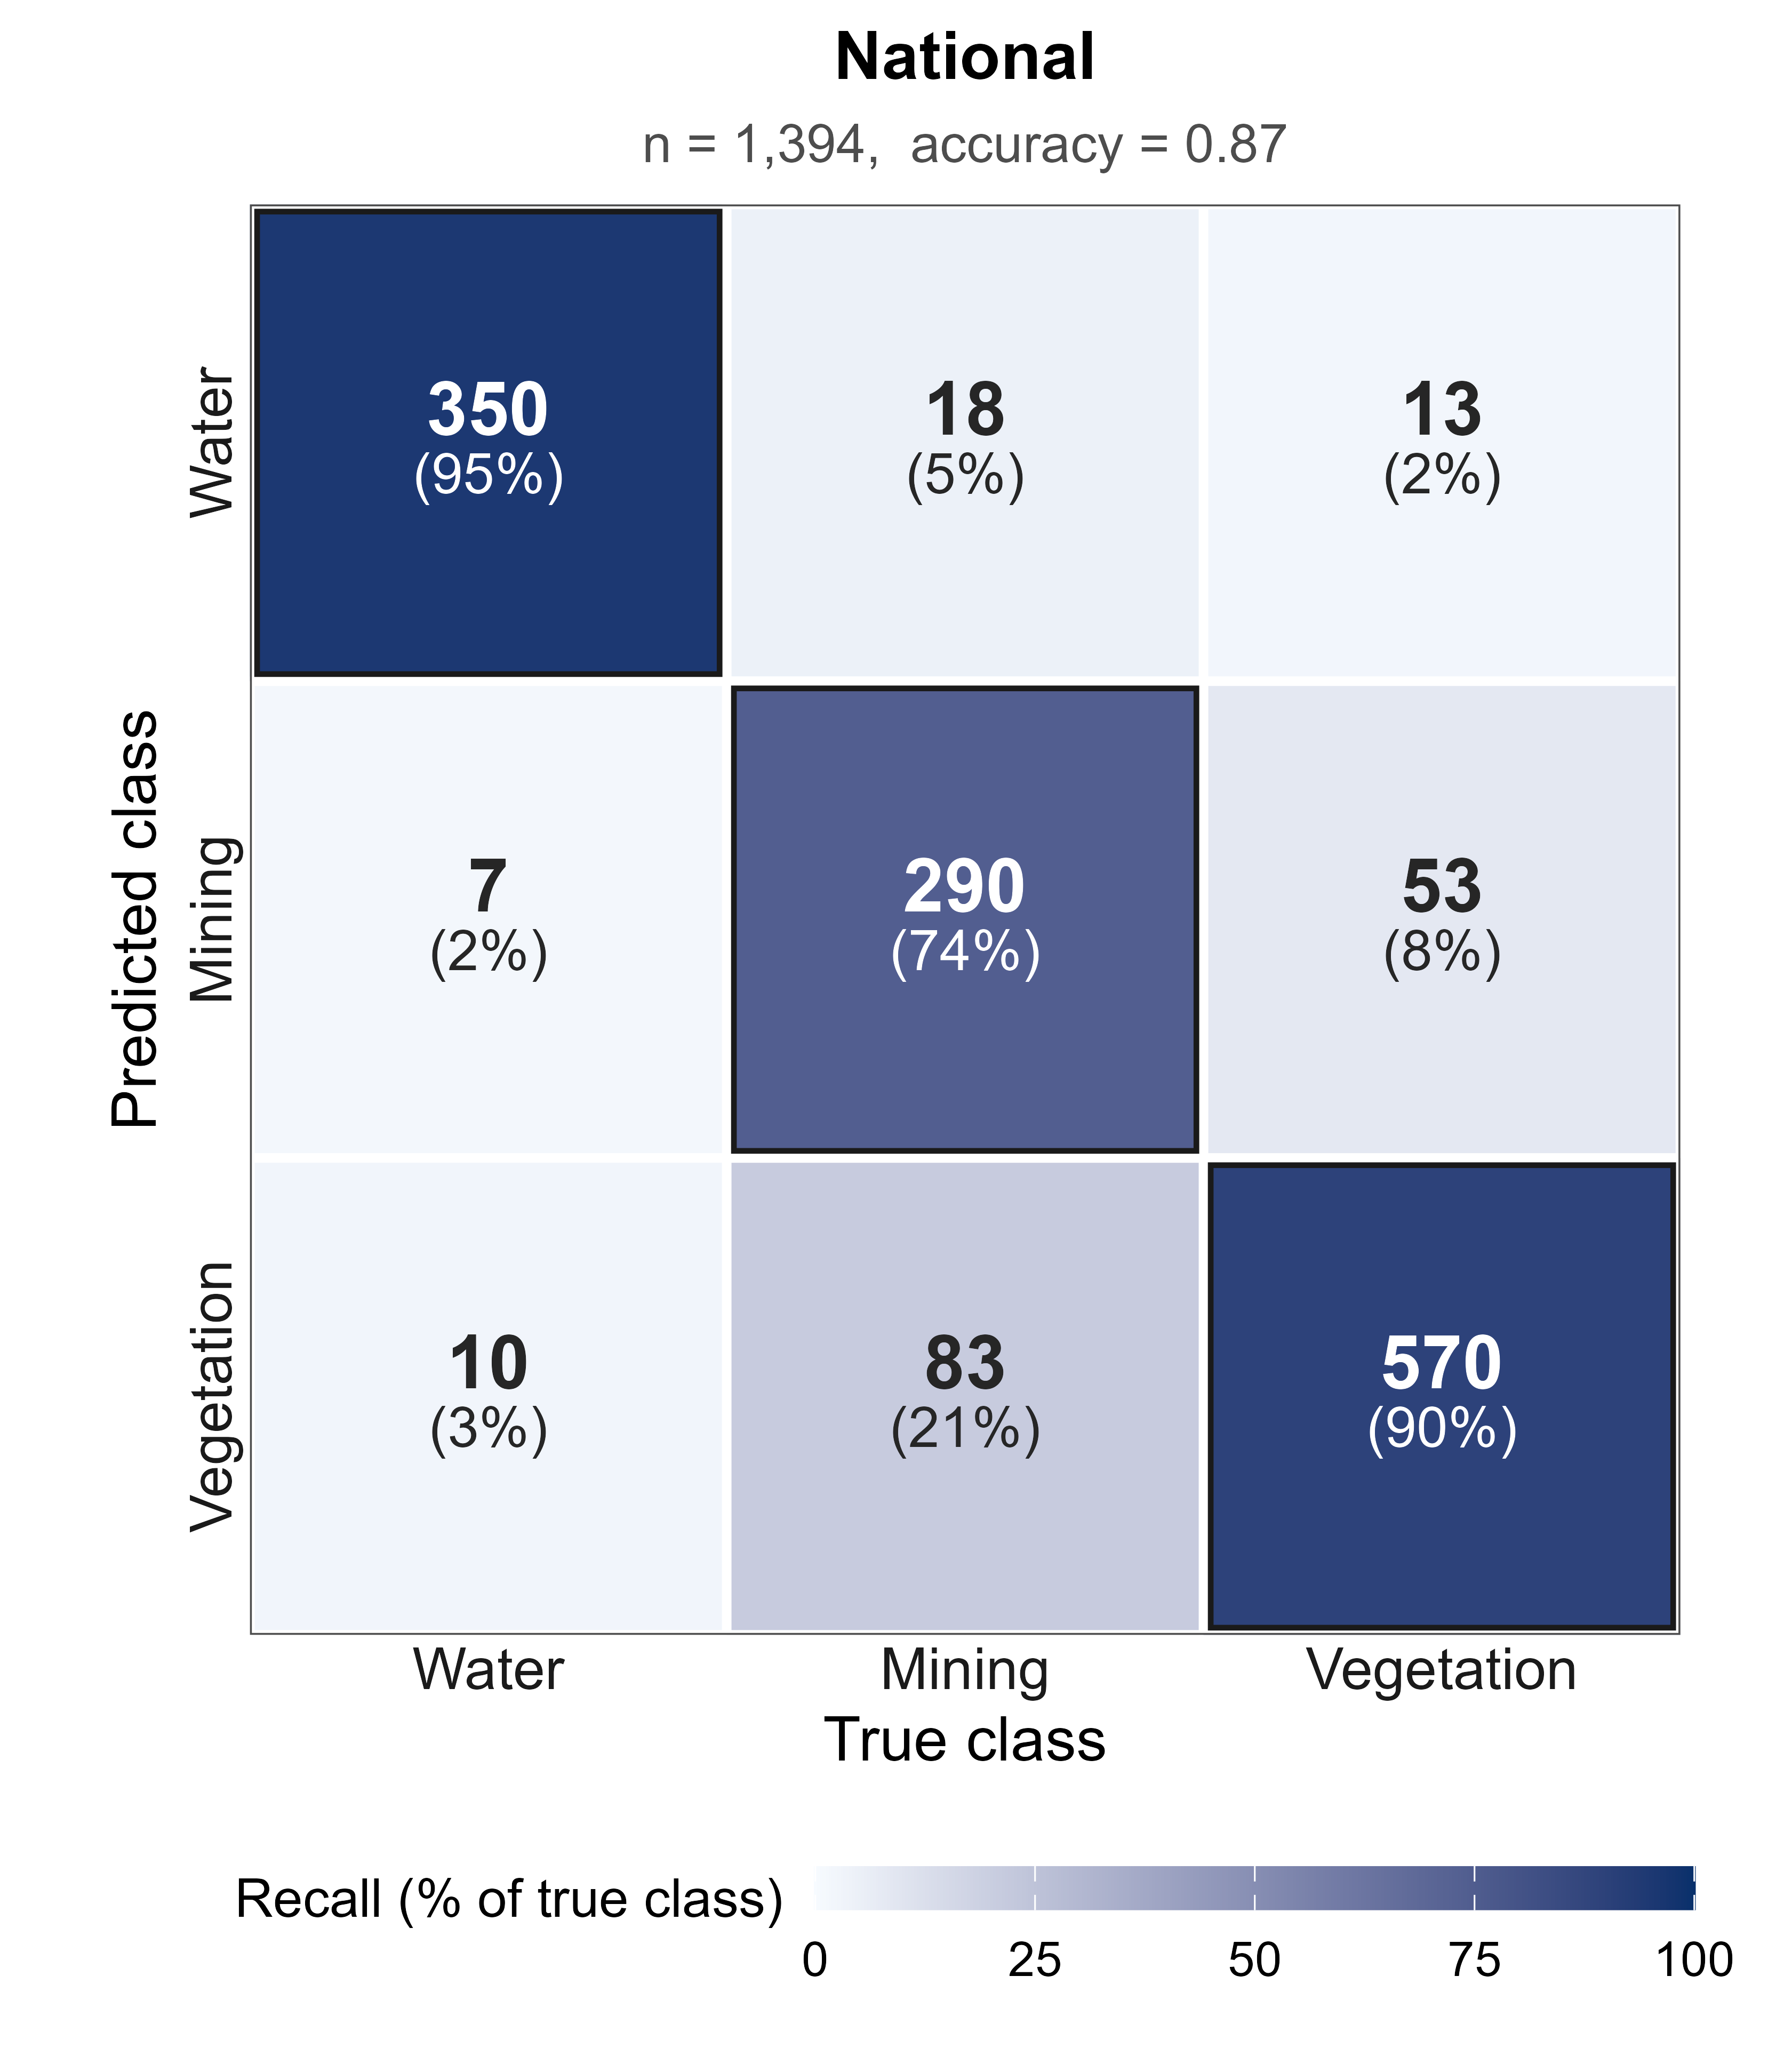
\includegraphics[width=0.85\textwidth]{figures/fig_confusion_national.png}
    \caption{Confusion matrix of the national model.}
    \label{fig:confusion_matrix}
\end{figure}

\begin{figure}[H]
  \centering
  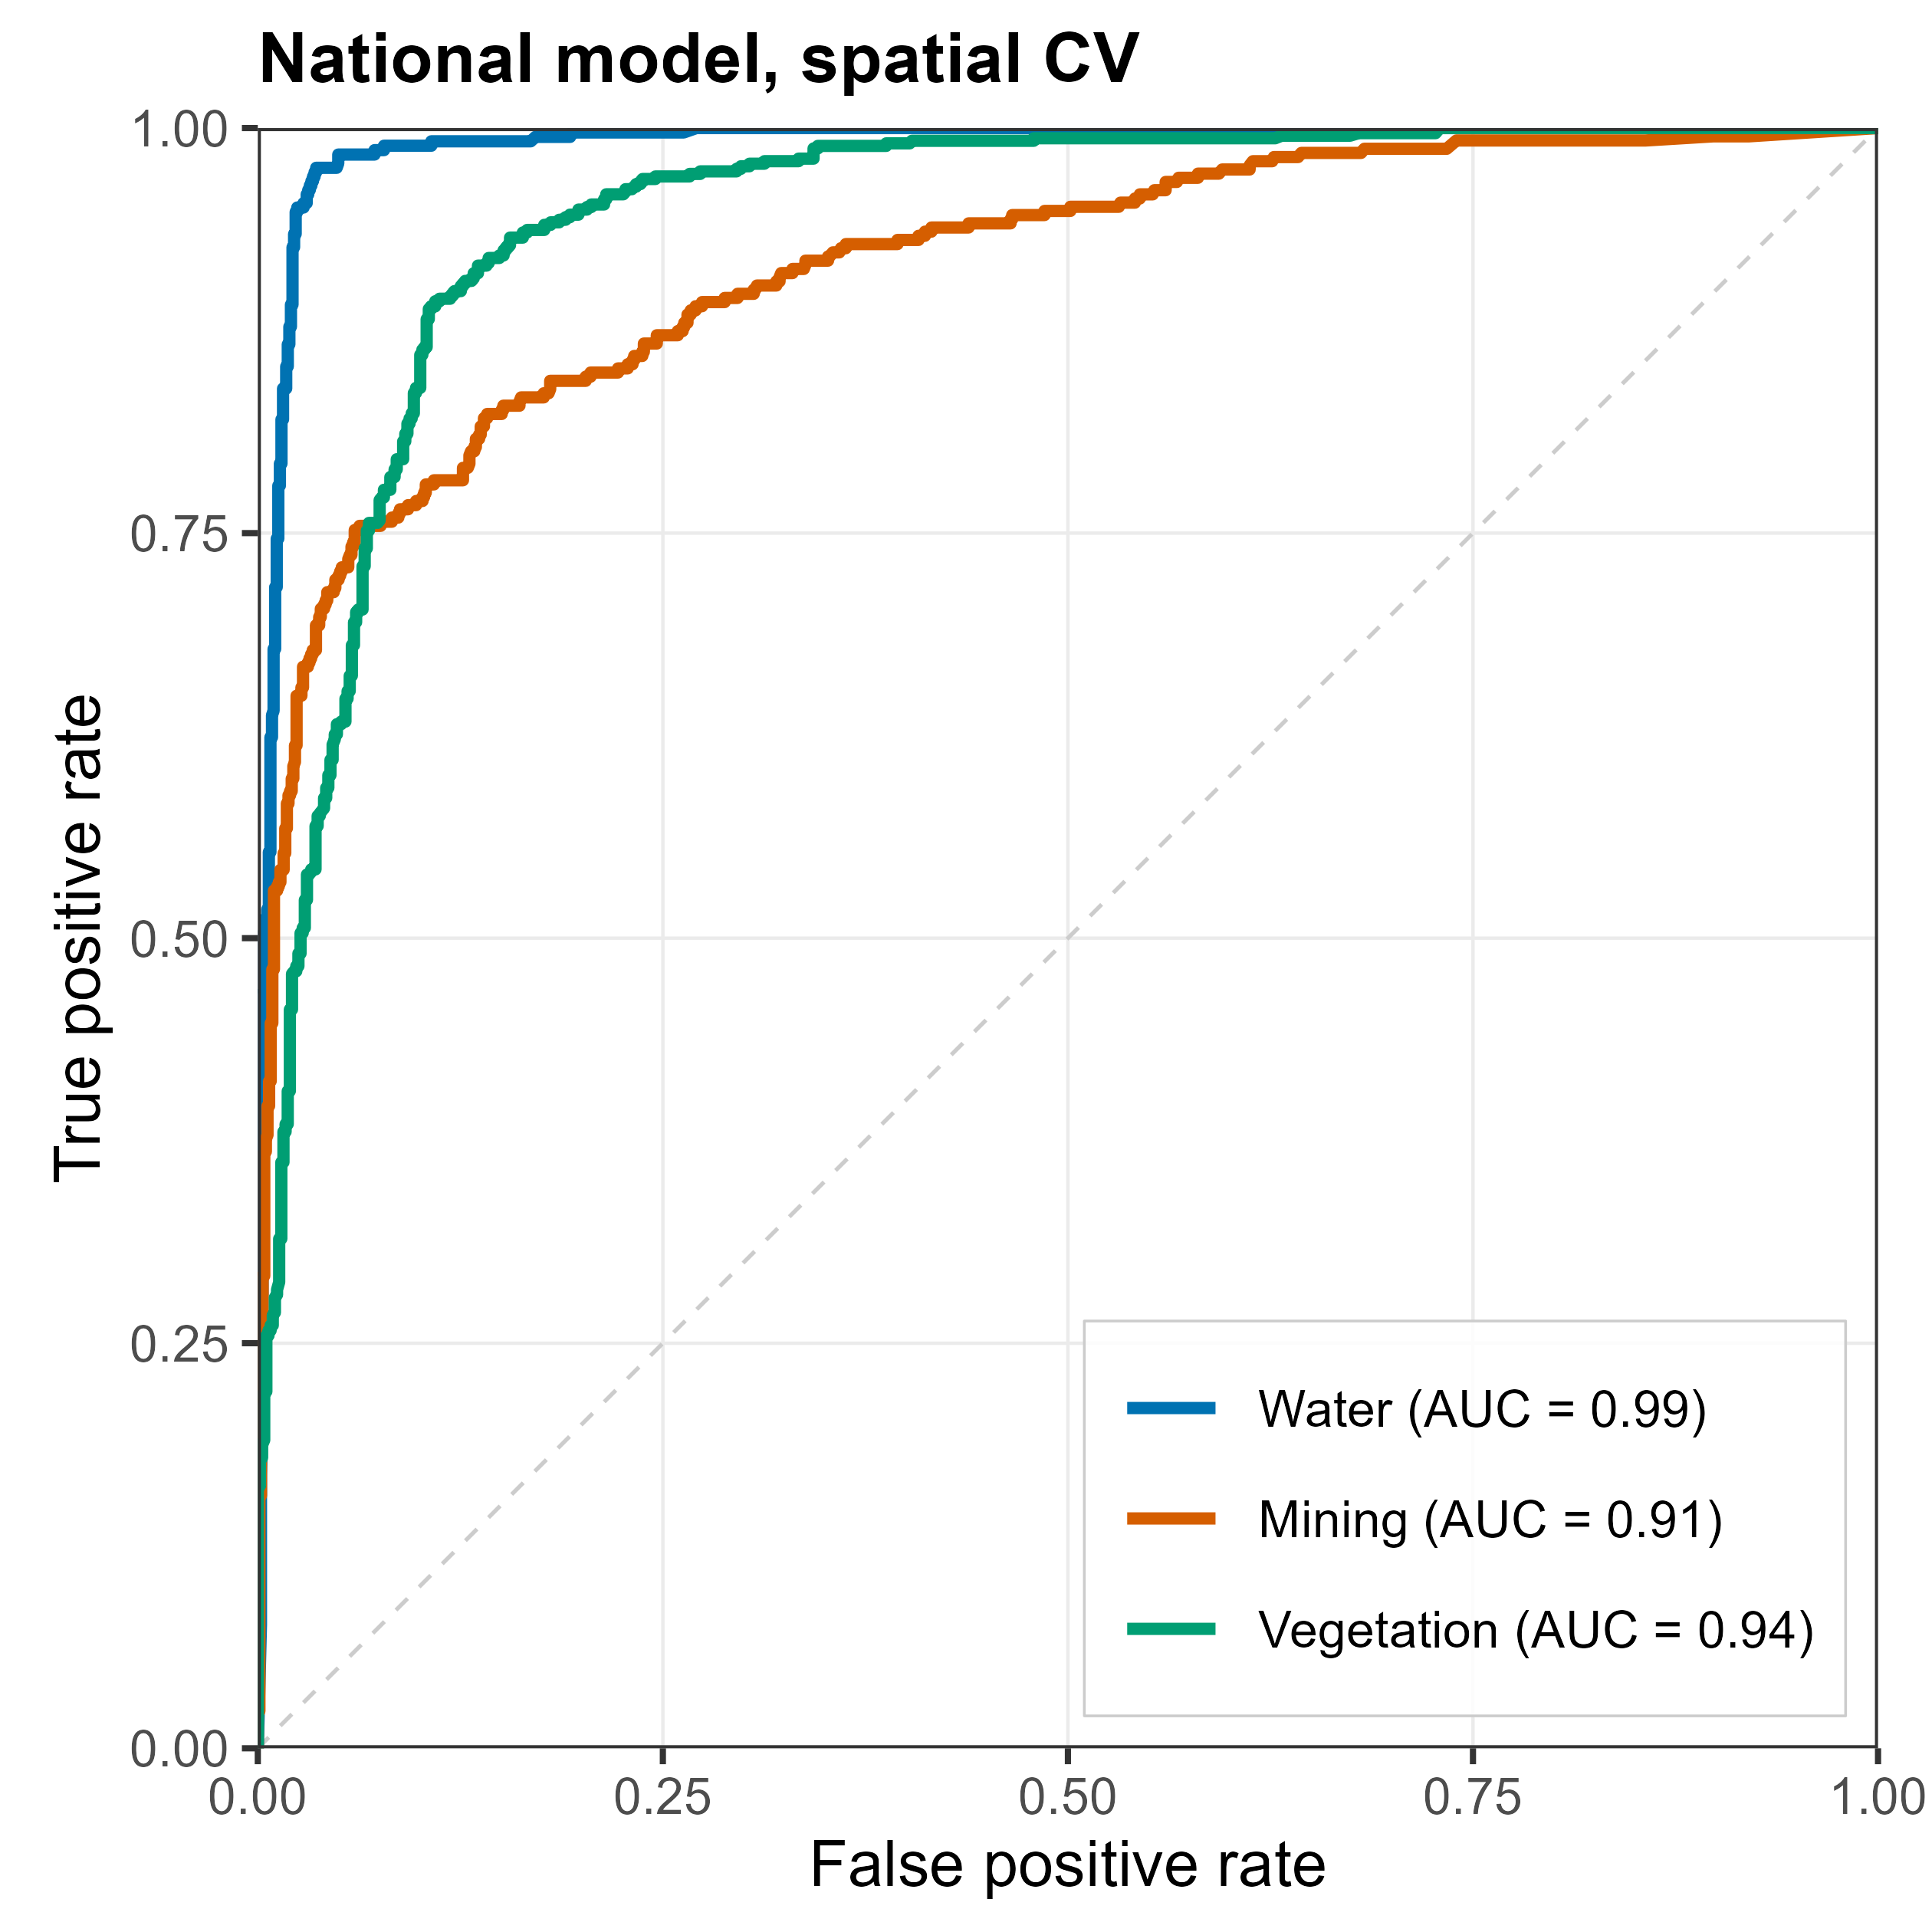
\includegraphics[width=0.6\textwidth]{figures/fig_roc_national.png}
  \caption{ROC curves of the national model (out-of-fold predictions, spatial
  cross-validation).}
  \label{fig:roc_national}
\end{figure}

\begin{figure}[H]
  \centering
  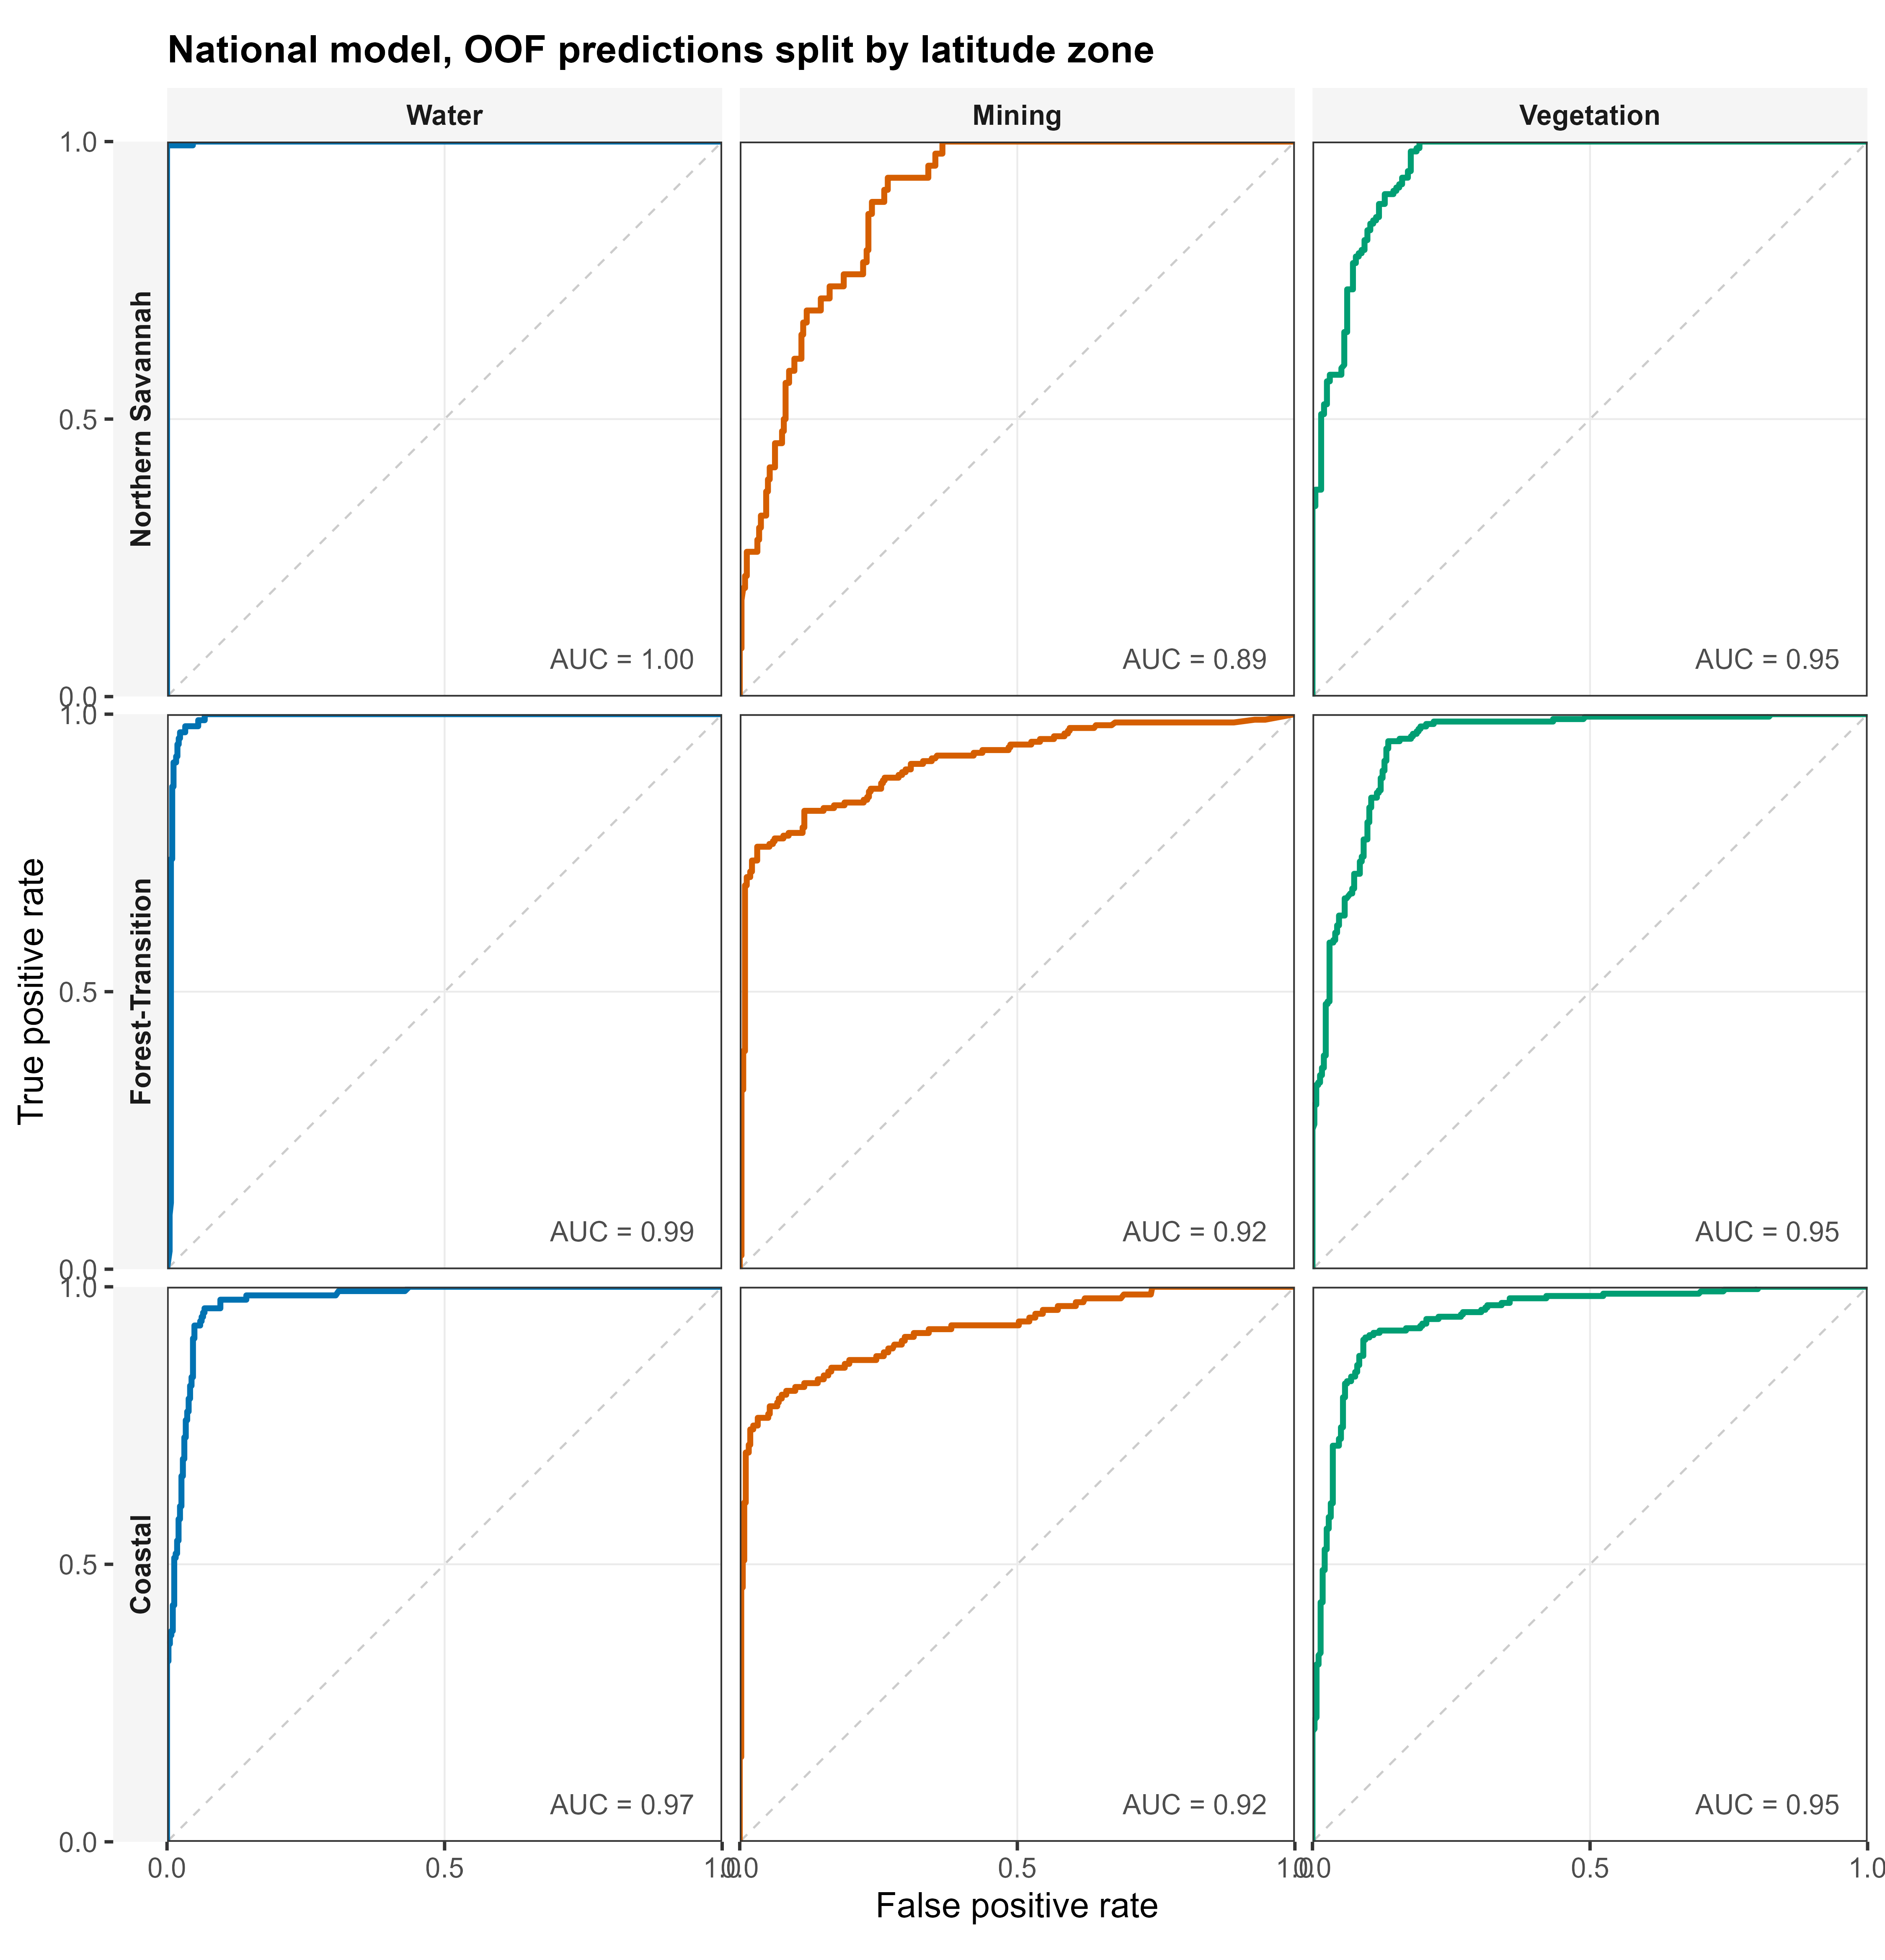
\includegraphics[width=0.85\textwidth]{figures/fig_roc_grid_zones.png}
  \caption{ROC curves of the national model per latitude zone.}
  \label{fig:roc_zones}
\end{figure}

The suggested national model (P0) achieved 0.87 (CI 0.83-0.91) overall accuracy (Mining F1 = 0.78) as compared to the national but 10-feature-focused model (M1) 0.858 (CI 0.82-0.9) (Mining F1 = 0.76), the zone-stratified and feature-focused model (M2) 0.87 (CI 0.86 to 0.88) (Mining F1 = 0.78), and the zone-specific but feature-uniform model (M3) 0.875 (CI 0.85-0.9) (Mining F1 = 0.79), with broadly overlapping 95 percent confidence intervals across all metrics (See Table~\ref{tab:benchmark_master} below). McNemar's tests indicate no statistically significant difference between my proposed national model and the zone-specific models but show that the full feature set (27 bands is significantly better than the national model with only 10 bands). These results suggest that statistical power was sufficient to determine that for my 1394 training samples distributed across three zones, there is no significant statistical difference between the national and zone-specific modelling approaches.

Random cross-validation inflated reported accuracy by only one percentage point (0.87 vs. 0.88) as compared to spatial blocking CV \citep{ploton2020Spatial,valavi2019Block}. This confirms that spatially proximate training and test samples share autocorrelated spectral signatures, and that the spatial CV estimates reported throughout this paper provide a more conservative and realistic assessment of model performances \citep{roberts2017Crossvalidation,valavi2019Block}, but are also not too far off in my use case and show only a minimal pessimism bias.

Table~\ref{tab:benchmark_master} reports all metrics across modelling
configurations using shared 5-fold spatial cross-validation folds with a
2.2~km buffer.

\begin{table}[H]
\centering
\small
\caption{Comparison of modelling approaches. Means from 5-fold spatially
blocked cross-validation (22.5~km blocks, 2.2~km variogram-derived buffer)
on $n = 1\,394$ training points; all spatial approaches share the same folds,
so test points are matched (a prerequisite for the McNemar tests). 95\% CI
for accuracy from the $t$-distribution across folds. Random CV repeats P0
with random folds of identical size and no buffer; the gap to P0 shows the
optimism of non-spatial validation.}
\label{tab:benchmark_master}
\resizebox{\textwidth}{!}{%
\begin{tabular}{lccccc}
\toprule
\textbf{Metric} & \makecell{\textbf{P0: National}\\\textbf{(27 bands)}\textsuperscript{a}} & \makecell{\textbf{M1: National}\\\textbf{(top-10 bands)}} & \makecell{\textbf{M2: Zone}\\\textbf{(literature bands)}} & \makecell{\textbf{M3: Zone}\\\textbf{(27 bands)}} & \makecell{\textbf{Random CV}\\\textbf{(P0)}} \\
\midrule
Overall accuracy & 0.870 [0.832--0.908] & 0.858 [0.820--0.895] & 0.869 [0.857--0.880] & 0.875 [0.850--0.900] & 0.879 [0.867--0.891] \\
Cohen's $\kappa$ & 0.796 & 0.777 & 0.794 & 0.803 & 0.810 \\
Water $F_1$      & 0.935 & 0.942 & 0.923 & 0.931 & 0.942 \\
Mining $F_1$     & 0.784 & 0.758 & 0.779 & 0.789 & 0.797 \\
Vegetation $F_1$ & 0.879 & 0.865 & 0.885 & 0.887 & 0.887 \\
Log-loss         & 0.405 & 0.434 & 0.441 & 0.376 & 0.342 \\
McNemar $p$ vs P0 & --- & 0.034 & 1.000 & 0.396 & --- \\
\bottomrule
\end{tabular}%
}
\par\vspace{0.4em}
\begin{minipage}{\textwidth}
\footnotesize
\textsuperscript{a}~Model used for all maps. M1 uses the decorrelated top-10
bands from the feature audit; M2 is the zone-specific approach with
literature-based bands per latitude zone; M3 uses zone models with the same
27 bands as P0, separating the effect of zoning from the effect of band
choice.
\end{minipage}
\end{table}

To assess where the model's cross-validated performance can be expected to hold, I computed the dissimilarity index (DI) and a resulting area of applicability (AOA) following \citet{meyer2021Predicting} (Figure \ref{fig:areaofa}). The DI was generally low across the detected mining area, indicating that my prediction locations were similar to the training data and that the spatial CV error estimates are likely transferable to most of the map. Higher DI values were spatially clustered rather than random, concentrating along river systems and around industrial mining sites, where conditions such as wet sediments or sparse vegetation regrowing on bare soil were underrepresented in the training data.

\begin{figure}[H]
    \centering
    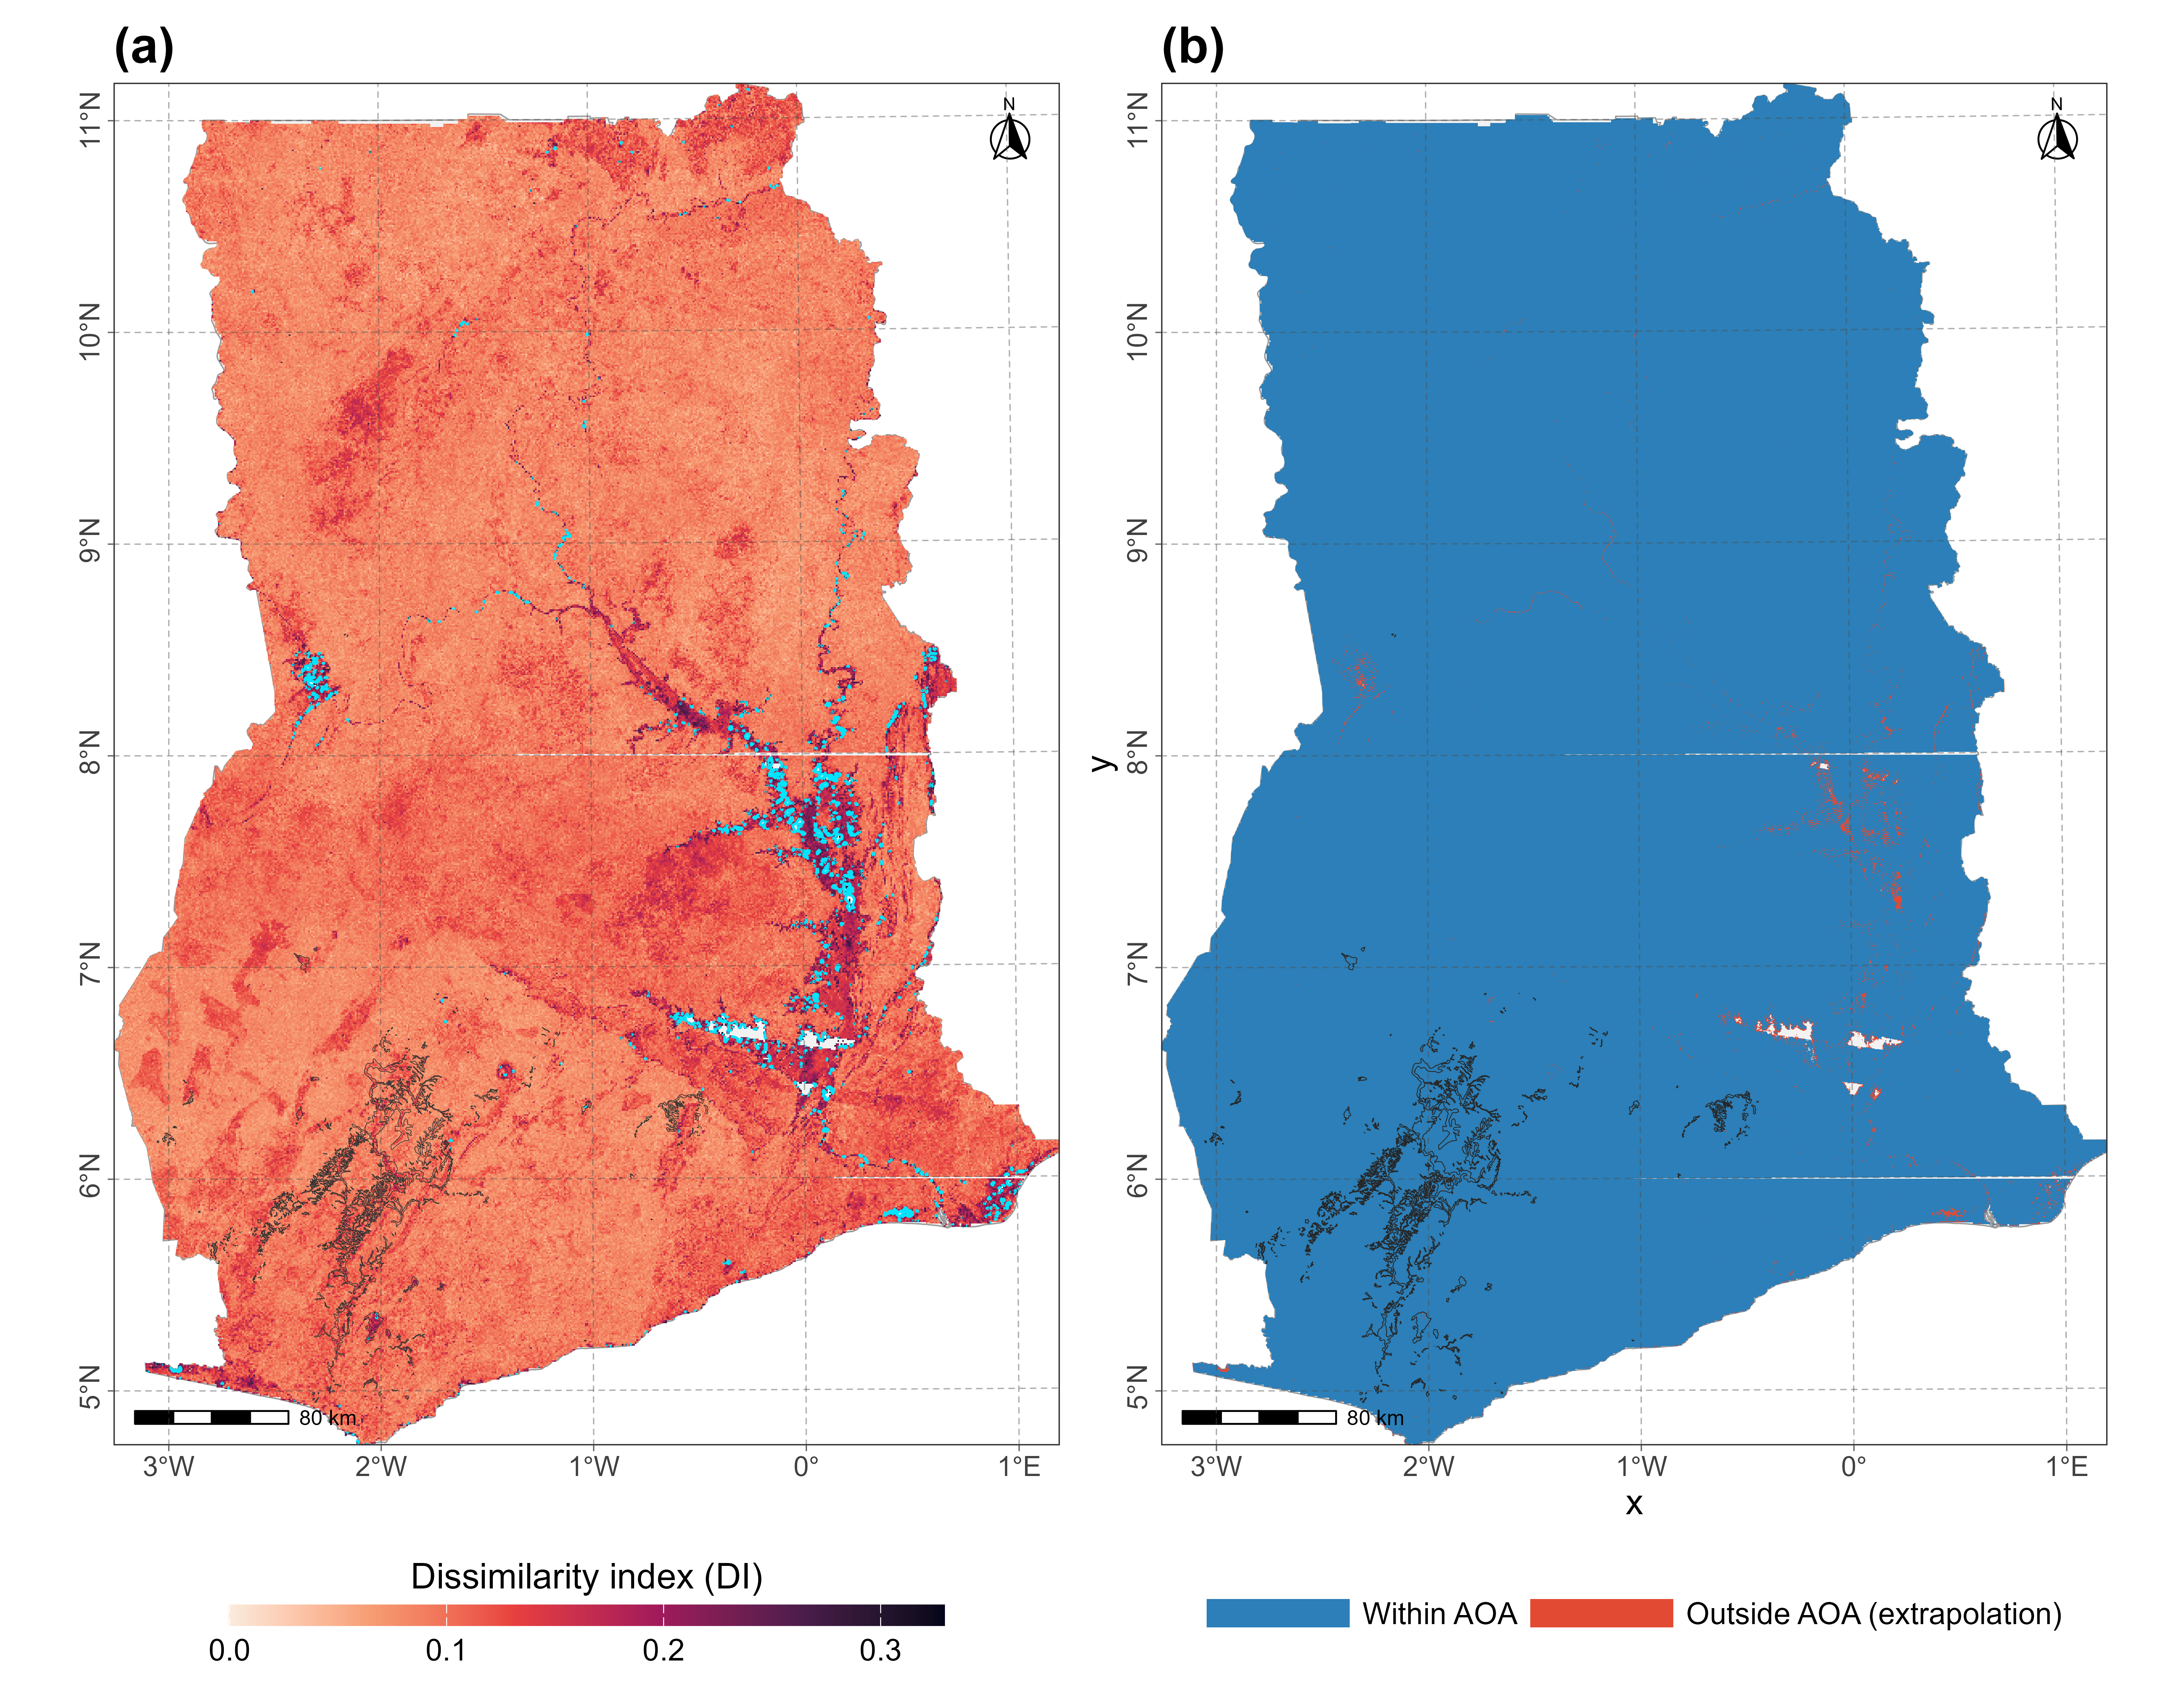
\includegraphics[width=0.9\textwidth]{figures/fig_aoa.png}
    \caption{Area of Applicability map. Dissimilarity Index (DI) on the left (a) shows darker and cyan areas that fall outside of what the model has seen before. Area of applicability (AoA) map on the right (b). Treshold from CV cross-validated DI. Mining polygons outlined.}
    \label{fig:areaofa}
\end{figure}

\section{Composite data quality assessment}
\label{app:quality}
For assessment of composite data quality, I extracted valid pixel counts, residual cloud probability, temporal standard deviation of key bands (NIR, RED, SWIR1), and missing data coverage from 15,000 stratified random sample points across all 20 annual composites (See appendix Table~\ref{tab:valid_pixels}, Figure~\ref{fig:valid_pixels}). The composite for year 2000 shows the lowest data availability. Mean valid pixel counts of 2.3–3.7 across my early study period up to 2011 reflect the limited data availability and quality of the Landsat 5/7 archive for tropical West Africa at the time. The Coastal zone maintained marginal coverage (below 5 valid pixels) through 2011, improving substantially after Landsat 8 became operational in 2013. Residual cloud probability in the final composites was effectively zero across all zone-years, indicating that the medoid selection procedure successfully excluded cloud-contaminated observations. Extreme outliers were excluded through band clipping.

\begin{table}[H]
\centering
\small
\caption{Mean valid pixel count per composite by zone for selected years.
Values below 5 (bold) indicate marginal coverage.}
\label{tab:valid_pixels}
\begin{tabular}{lccc}
\toprule
\textbf{Year} & \textbf{Northern Savannah} & \textbf{Forest-Transition} & \textbf{Coastal} \\
\midrule
2000 & 3.6 & 3.4 & \textbf{2.4} \\
2001 & 6.0 & 5.5 & \textbf{4.3} \\
2005 & 6.4 & 5.7 & \textbf{4.8} \\
2010 & 8.9 & 6.1 & \textbf{3.7} \\
2013 & 14.9 & 13.5 & 9.3 \\
2015 & 28.0 & 24.6 & 17.8 \\
2019 & 33.8 & 28.4 & 22.0 \\
\bottomrule
\end{tabular}
\end{table}

Residual cloud probability was close to zero in all zone-years, but the low
number of valid pixels in early years shows the limited Landsat data
availability in cloudy areas.

\begin{figure}[H]
  \centering
  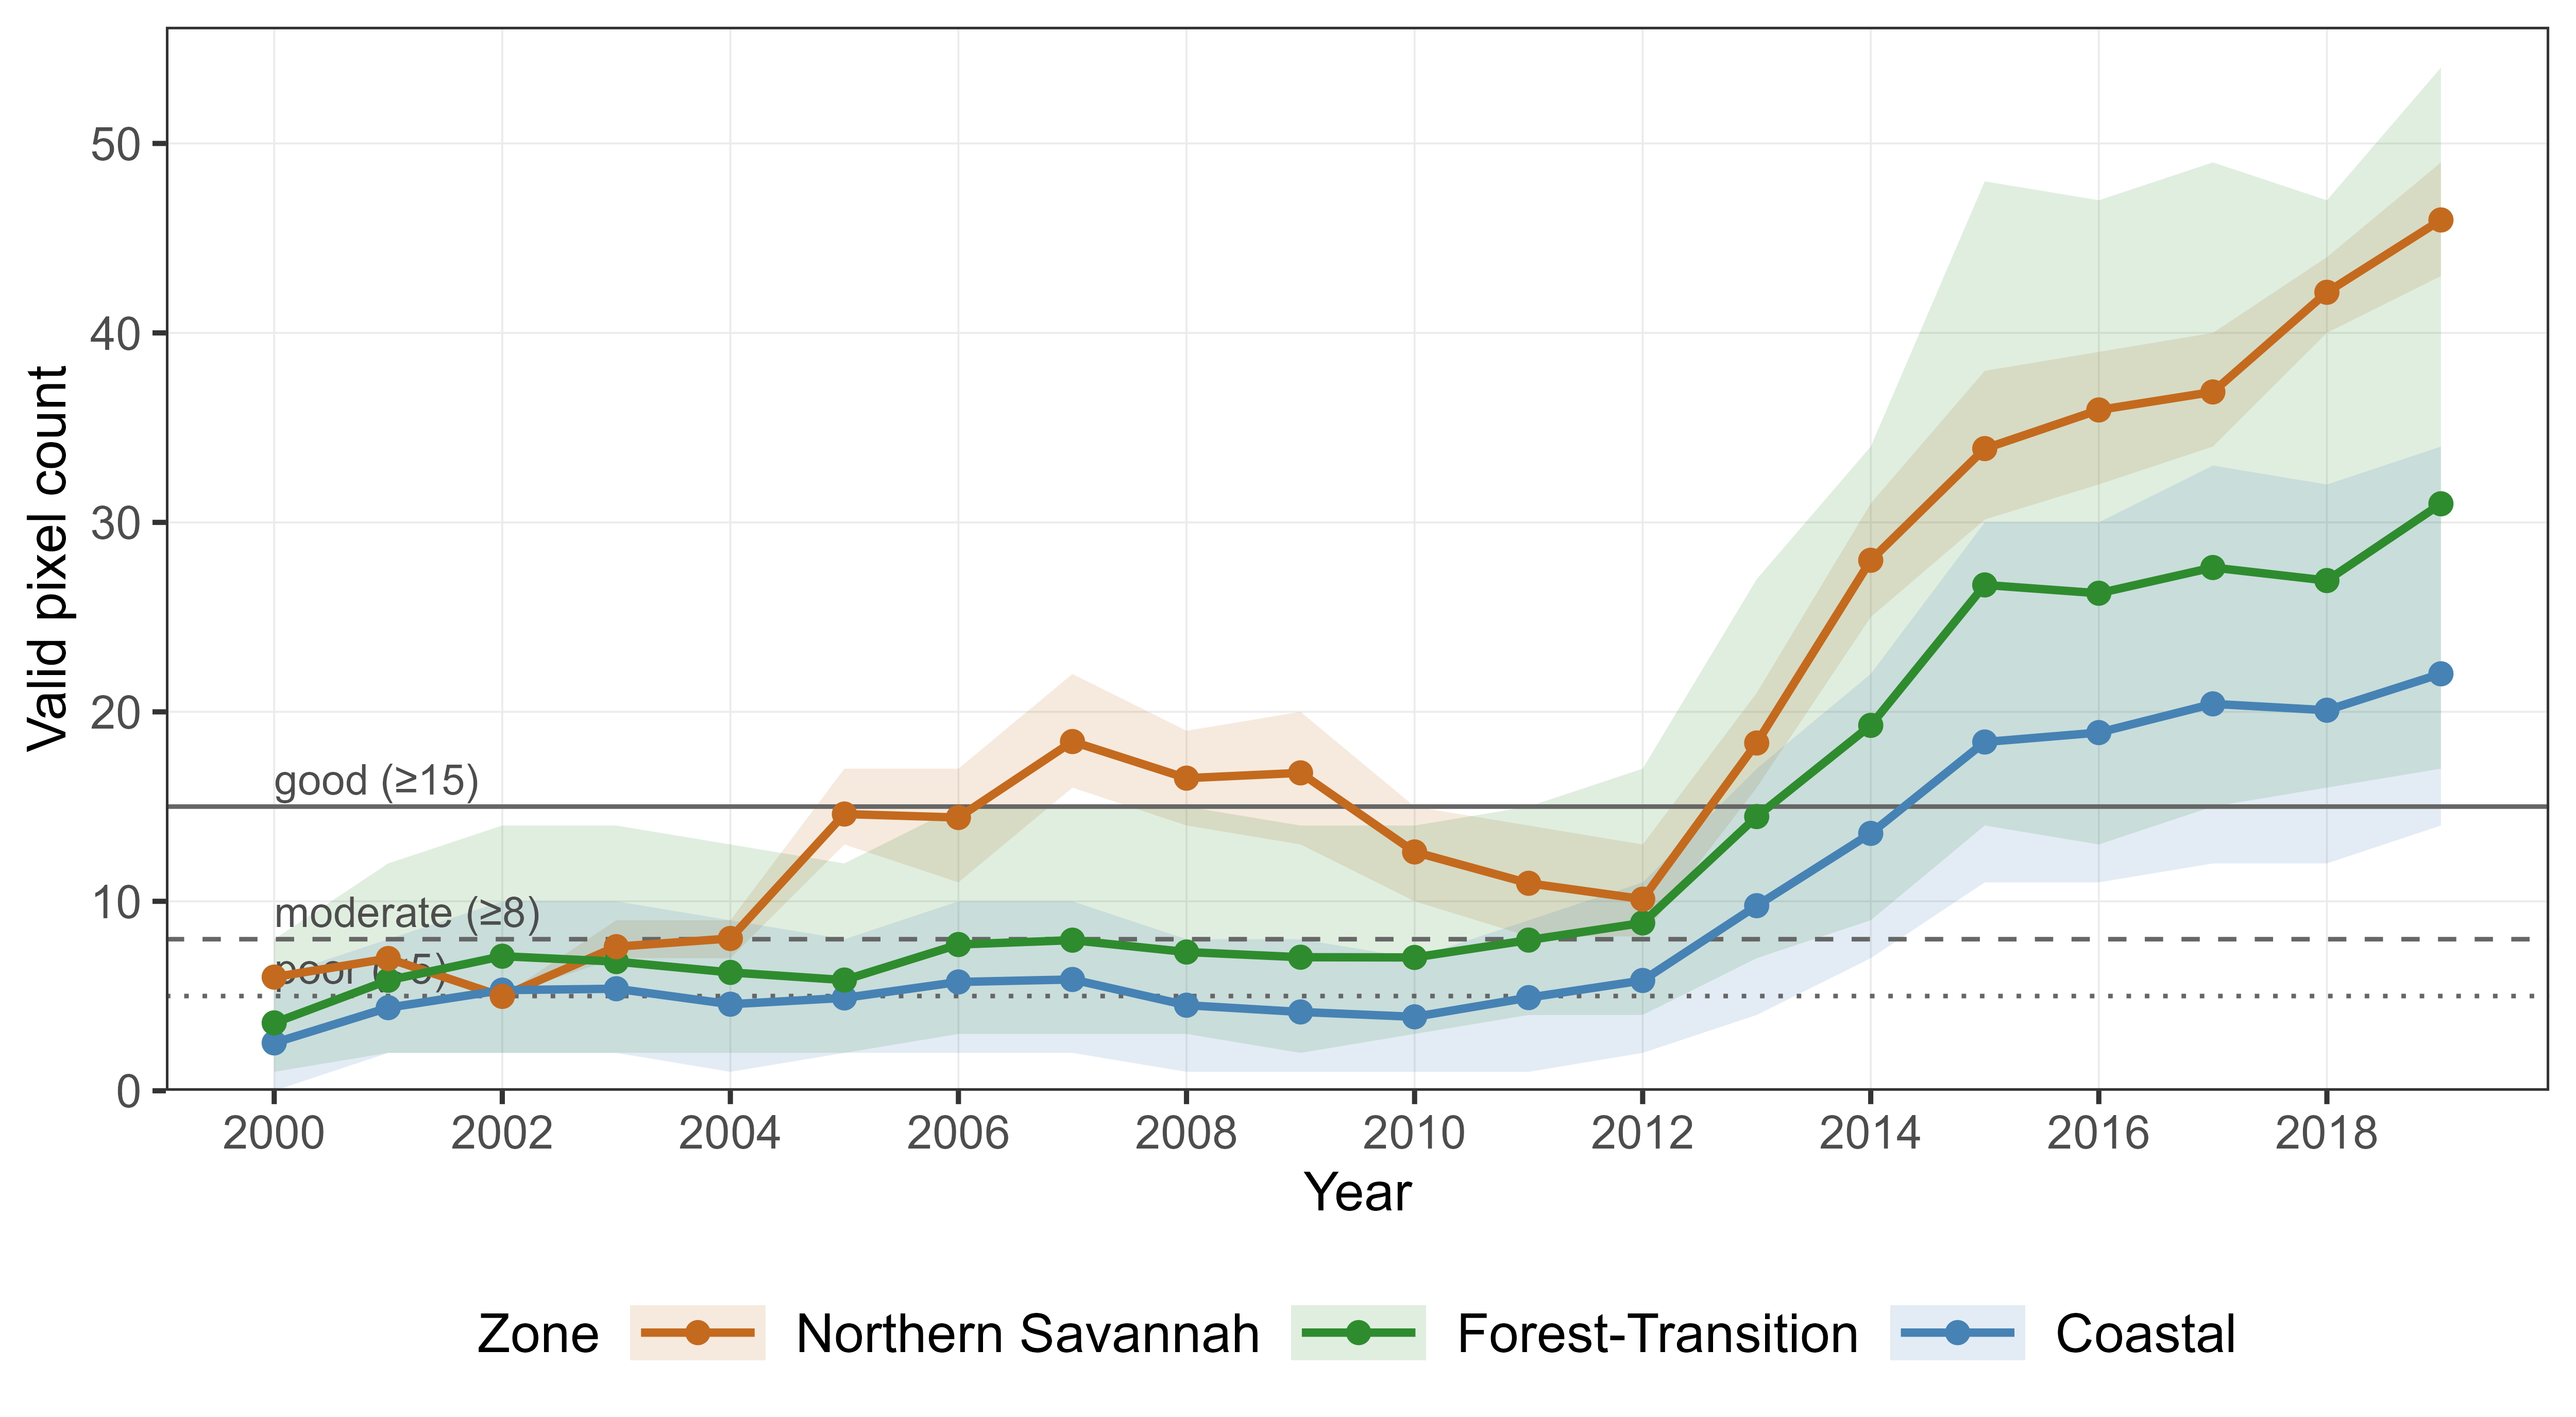
\includegraphics[width=0.9\textwidth]{figures/fig_valid_pixel_count.png}
  \caption{Valid pixel count per composite year within the study area. The
  step increase after 2012 reflects Landsat~8 availability. Horizontal lines
  indicate quality thresholds.}
  \label{fig:valid_pixels}
\end{figure}

\section{Industrial mining sites}
\label{app:industrial}

To check whether the transition rule is too aggressive, I visualised four
industrial mines with known start dates (Figure~\ref{fig:industrial_mines}).

As visible, the RF and constraining approach manages to predict industrial mining onset reliably, even in earlier years.

\begin{figure}[H]
  \centering
  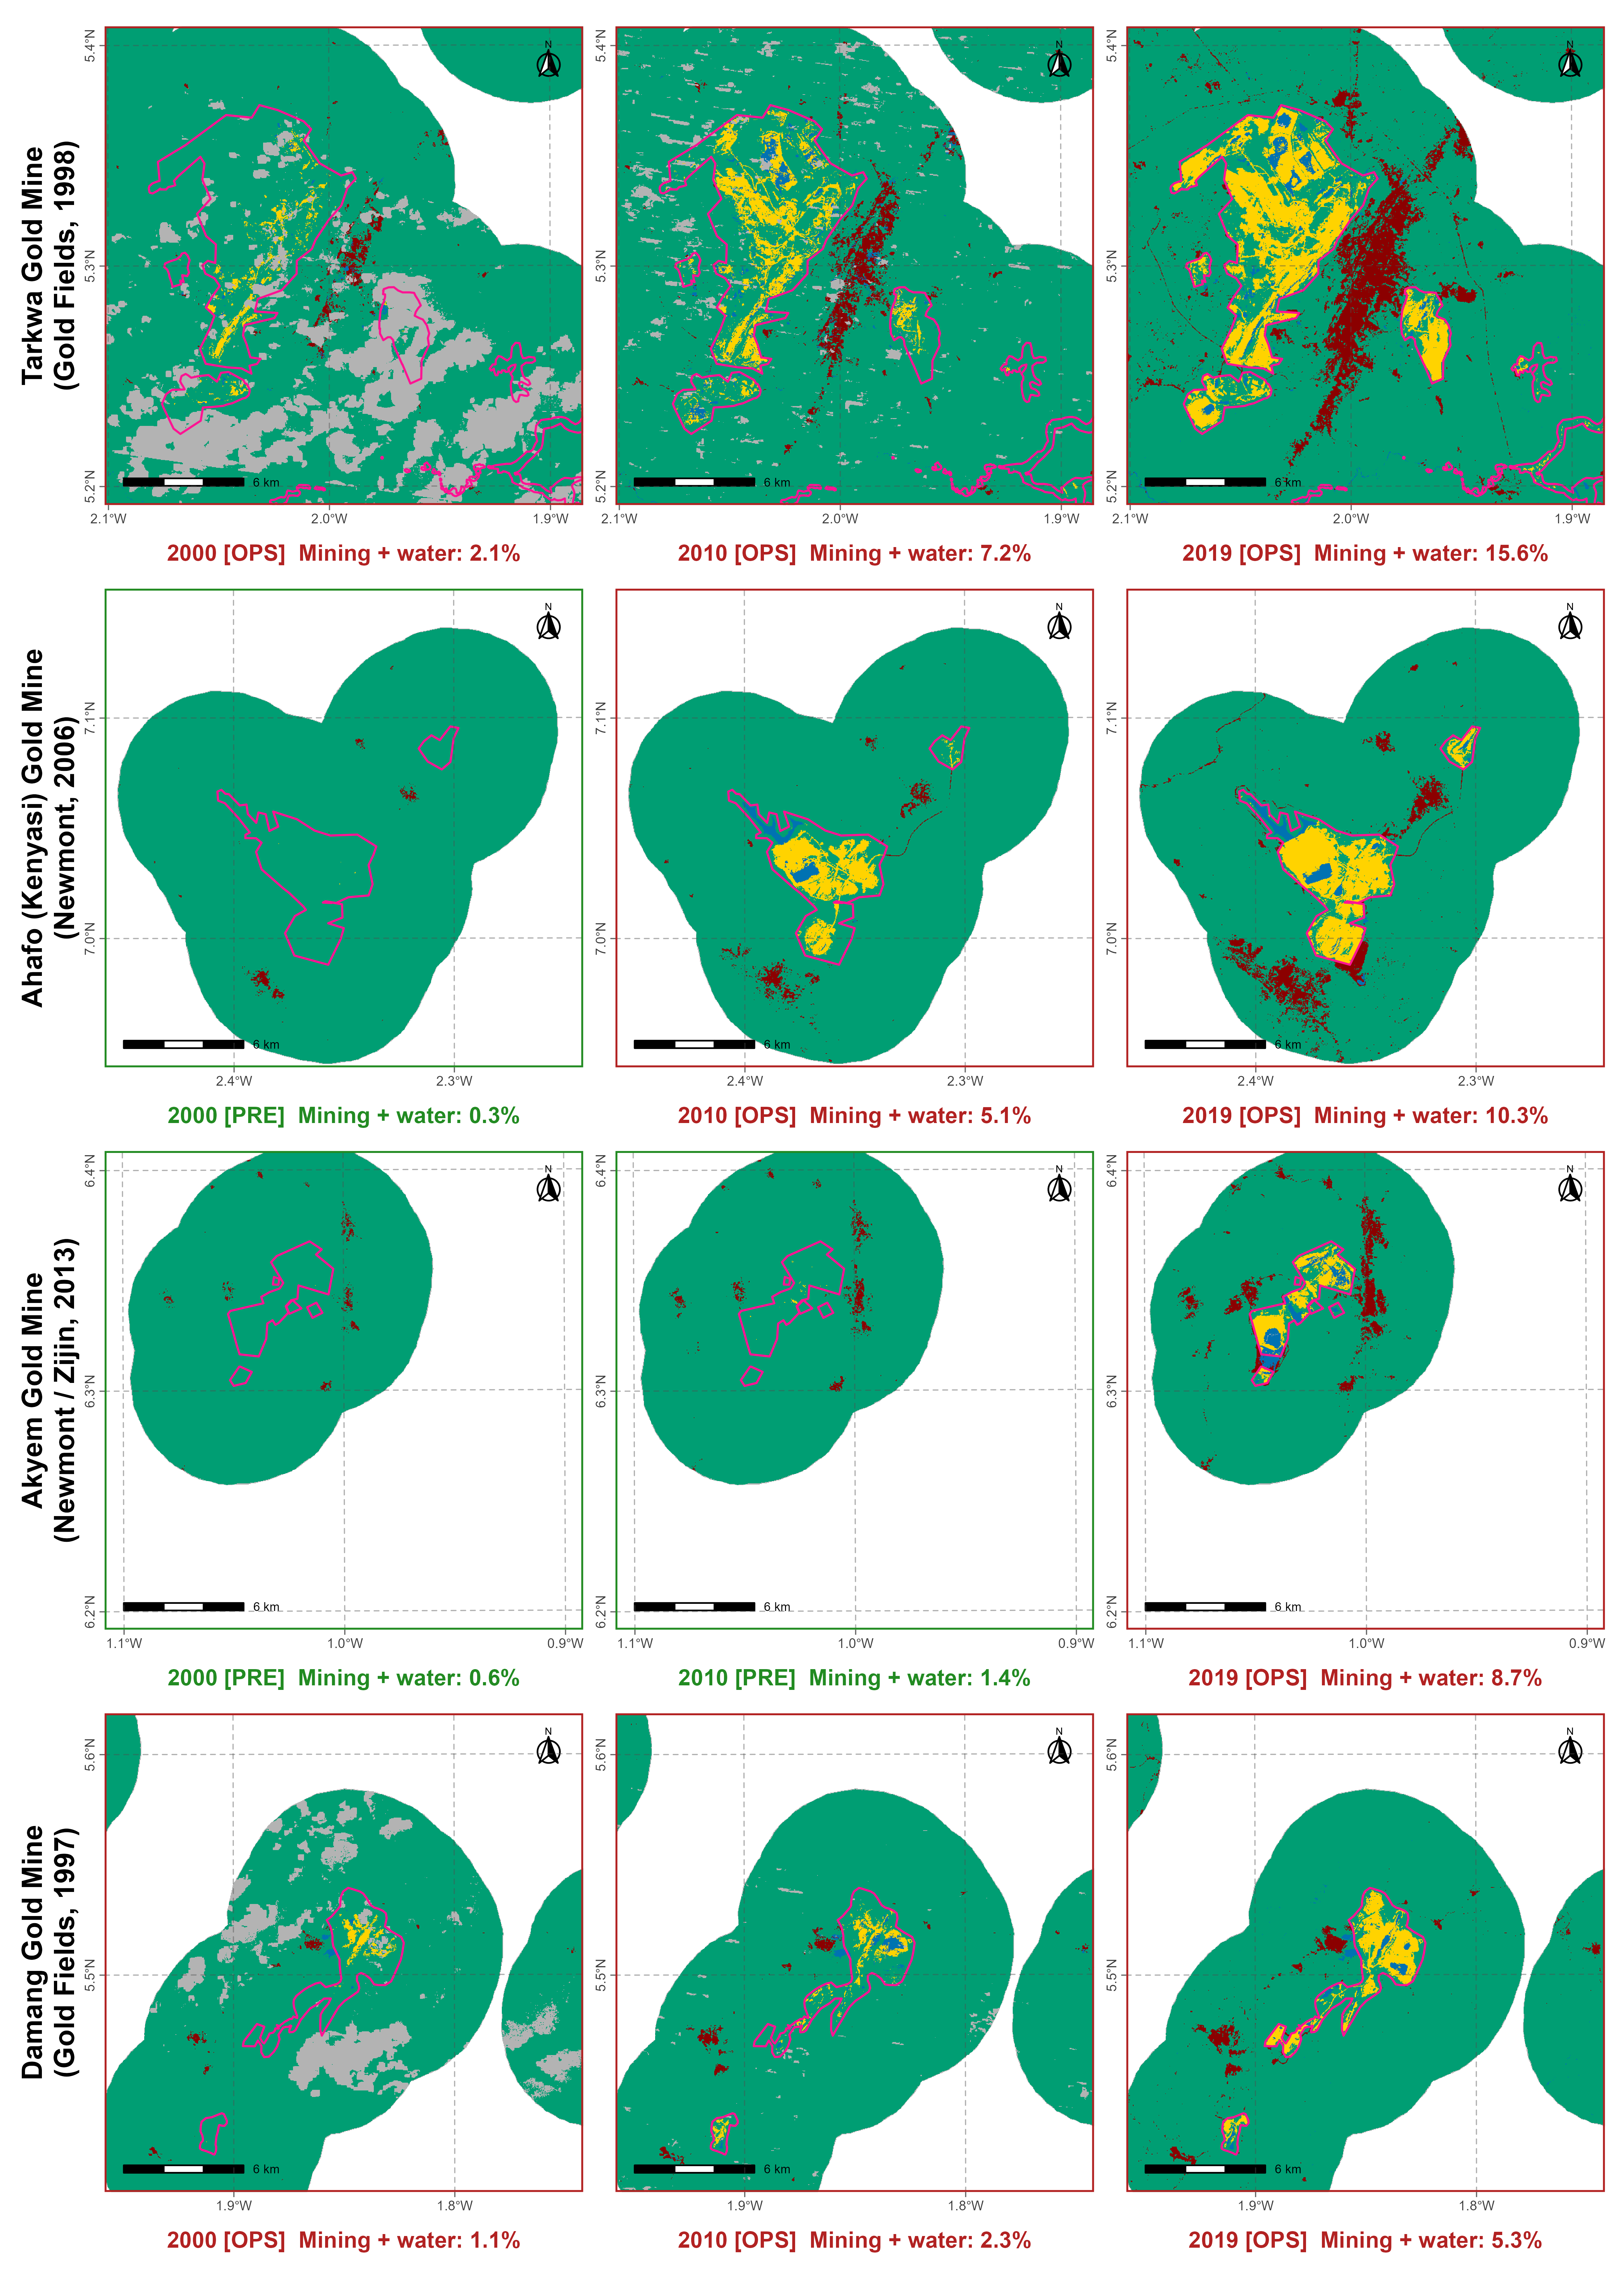
\includegraphics[width=0.9\textwidth]{figures/fig_industrial_mines_appendix.png}
  \caption{Constrained classification of four large industrial mines in 2000,
  2010 and 2019, with mining polygons outlined. [PRE] = before, [OPS] = after
  the documented start of operations.}
  \label{fig:industrial_mines}
\end{figure}

\section{CNN validation of industrial mining onset}
\label{app:cnn}
\subsection{CNN comparison}
As a consistency check, I trained a convolutional neural network (patch classifier)\citep{lecun1998Gradientbased} on 32x32 pixel tiles of the 2019 industrial mine footprints and applied the model backwards to earlier years. I used footprints of 16 industrial mines from the \citet{maus2022update} polygons with a 5~km buffer around each mine and its Voronoi cell, so that mines did not share area. The CNN took six reflectance bands, eight spectral and teture indices, and a validaty mask for classification. The CNN consists of three convolution blocks (two 3x3 convolutions with batch normalisation and ReLu; \citep{ioffe2015Batch}), used max-, and global average pooling \citep{lin2014Network}, dropout against overfitting \citep{srivastava2014Dropout}, and a sigmoid output. Whilst positive patches came from the industrial mining footprint of the 2019 composite, the negative examples came from mining cells outside the mining footprints (40\%), surrounding landscape (20\%), bright surfaces (20\%), and random background (20\%), so that the network had to also distinguish industrial from artisanal mining. Cross validation followed \citet{roberts2017Crossvalidation} with mines closer than 20km from each other grouped together and then assigned to four spatial folds, so the CNN could not memorise the mine it was dating. I calibrated year-specific detection thresholds for industrial mines on held-out imagery to assess sensor differences between Landsat 5/7 and 8 (See table~\ref{tab:app_cnn_rf_onsets}). Mining onset (T10) was then defined as the first year in which at least 10\% of a mine's 2019 mined extent (Mining and Water cells, vegetation excluded) was detected in three consecutive years. For the five mines established within the study period\footnote{E.g. Ahafo (2005).}, RF onsets are compared to the CNN ones and the actual mine establishment and production information from the Ghana Minerals Commission \citep{Industrystatistics}. The table below shows that the RF scored better than the CNN at mining onset detection.

Namdini mine which established in 2021 serves as a negative control here.

\begin{table}[H]
\centering
\caption{Onset of industrial mining per mine: random forest (RF)
classification versus an independent convolutional neural network (CNN).}
\label{tab:app_cnn_rf_onsets}
\small
\setlength{\tabcolsep}{3pt}
\begin{threeparttable}
\begin{tabular}{@{}lrlrrccr@{}}
\toprule
 & & & \multicolumn{2}{c}{2019 extent (ha)} & \multicolumn{2}{c}{Onset (T10)} & \\
\cmidrule(lr){4-5}\cmidrule(lr){6-7}
Mine & Est. & MinCom\tnote{a} & Mined & Threshold & RF & CNN & $\Delta$\tnote{b} \\
\midrule
\multicolumn{8}{@{}l}{\textit{Established 2001--2019}}\\
Chirano & 2005 & $\leq$2013 & 498 & 50 & 2005 & 2013 & $+8$ \\
Ahafo & 2006 & $\leq$2013 & 1,971 & 197 & 2005 & 2006 & $+1$ \\
Edikan & 2011 & $\leq$2013 & 1,148 & 115 & 2011 & 2012 & $+1$ \\
Nzema & 2011 & $\leq$2013 & 260 & 26 & 2006 & 2011 & $+5$ \\
Akyem & 2013 & 2013 & 752 & 75 & 2012 & 2004 & $-8$ \\
\midrule
\multicolumn{8}{@{}l}{\textit{Established before 2000}}\\
Nsuta & 1916 & $\leq$2013 & 489 & 49 & 2004 & 2002 & $-2$ \\
Bogoso & 1990 & $\leq$2013 & 427 & 43 & 2003 & 2004 & $+1$ \\
Iduapriem & 1992 & $\leq$2013 & 871 & 87 & $\leq$2000 & $\leq$2000 & -- \\
Asanko & 1997 & 2016 & 1,276 & 128 & 2012 & $\leq$2000 & $-12$\tnote{c} \\
Bibiani & 1997 & $\leq$2013 & 177 & 18 & $\leq$2000 & 2001 & $+1$\tnote{c} \\
Damang & 1997 & $\leq$2013 & 838 & 84 & $\leq$2000 & $\leq$2000 & -- \\
Tarkwa & 1998 & $\leq$2013 & 2,482 & 248 & 2001 & $\leq$2000 & $-1$\tnote{c} \\
Wassa & 1998 & $\leq$2013 & 361 & 36 & $\leq$2000 & 2006 & $+6$\tnote{c} \\
\midrule
\multicolumn{8}{@{}l}{\textit{Excluded from CNN training and agreement statistics\tnote{d}}}\\
Obuasi & 1897 & $\leq$2013 & 42 & 10 & $\leq$2000 & 2002 & $+2$\tnote{c} \\
Awaso & 1941 & $\leq$2013 & 142 & 14 & $\leq$2000 & n.d. & -- \\
Prestea & 1990 & $\leq$2013 & 398 & 40 & 2002 & 2006 & $+4$ \\
\bottomrule
\end{tabular}
\begin{tablenotes}[flushleft]
\footnotesize
\item \textit{Notes}: Est.\ = documented start of operations. Mined = 2019
RF mining and water cells inside the mine footprint (mining polygons within
5~km of the mine, split between neighbouring mines); vegetation inside the
polygons is not counted. T10 = first year in which at least 10\% of the 2019
mined extent (Threshold; minimum 10~ha) is detected in 3 consecutive
observed years. CNN detection thresholds are calibrated per year to a 1\%
background false-positive rate. $\leq$ = left-censored (already met in the
first observed year). n.d.\ = not detected.
\item[a] First reported large-scale production in Minerals Commission
statistics (company-level data from 2013; $\leq$2013 = producing in the
first reported month).
\item[b] CNN minus RF onset in years.
\item[c] One of the two onsets is left-censored, so the difference is a bound.
\item[d] Obuasi and Prestea are mainly underground operations; Awaso is the
only bauxite mine. The negative control Namdini (established 2021) lies
outside the RF prediction area.
\end{tablenotes}
\end{threeparttable}
\end{table}

\end{document}